% !TeX spellcheck = en_GB
%%%%%%%%%%%%%%%%%%%%%%%%%%%%%%%%%%%%%%%%%%%%%%%%%%%%%%%%%%%%%%%%%%%%%%%%%%%%%%%%
% Preamble                                                                     %
%%%%%%%%%%%%%%%%%%%%%%%%%%%%%%%%%%%%%%%%%%%%%%%%%%%%%%%%%%%%%%%%%%%%%%%%%%%%%%%%

\documentclass[12pt,a4paper,openbib]{report}

\usepackage{estilo_pfc}
\usepackage{longtable}
\usepackage{musixtex}
\usepackage{cite}
\usepackage{titlesec}
\usepackage{fancyvrb}
\usepackage[export]{adjustbox}
\usepackage{relsize}

\author{AUTOR/A DEL PROYECTO}
\date{FECHA DEL PROYECTO}

%%%%%%%%%%%%%%%%%%%%%%%%%%%%%%%%%%%%%%%%%%%%%%%%%%%%%%%%%%%%%%%%%%%%%%%%%%%%%%%%
% Body                                                                         %
%%%%%%%%%%%%%%%%%%%%%%%%%%%%%%%%%%%%%%%%%%%%%%%%%%%%%%%%%%%%%%%%%%%%%%%%%%%%%%%%

\begin{document}

 %%%%%%%%%%%%%%%%%%%%%%%%%%%%%%%%%%%%%%%%
 % Definición de comandos               %
 %%%%%%%%%%%%%%%%%%%%%%%%%%%%%%%%%%%%%%%%

 \newcommand{\paginaenblanco}{\mbox{}\thispagestyle{empty}\newpage}
 \newcommand{\exedout}{%
   \rule{0.8\textwidth}{0.5\textwidth}%
 }

 %%%%%%%%%%%%%%%%%%%%%%%%%%%%%%%%%%%%%%%%
 % Preliminares documento               %
 %%%%%%%%%%%%%%%%%%%%%%%%%%%%%%%%%%%%%%%%

 \begin{titlepage}
\begin{center}

\includegraphics[width=5cm]{imagenes/anagramaUDC.png}\\[0.5cm]
{\textsc{Facultad de Informática}} \\
{\large \textsc{Departamento de Computación}} \\[1cm]
{\Large \textsc{Herramienta para armonización musical mediante Answer Set Programming}} \\[2cm]
\vfill
\begin{flushright}
\begin{tabular}{ll}
\textbf{Autores:}	 & Martín Prieto, Rodrigo \\
					 & Cabalar Fernández, Pedro \\
& \\
\multicolumn{2}{r}{\small \emph{A Coruña, a 1 de junio de 2015}} \\
\end{tabular}
\end{flushright}
\end{center}
\end{titlepage}

 %%%%%%%%%%%%%%%%%%%%%%%%%%%%%%%%%%%%%%%%%%%%%%%%%%%%%%%%%%%%%%%%%%%%%%%%%%%%%%%%

\begin{abstract}
\thispagestyle{empty}
Este proyecto consiste en el desarrollo de una herramienta inteligente de ayuda a la armonización capaz de comprender la armonía presente en una partitura y completar tramos de la misma, llegando incluso a poder crear nuevas voces de la nada que sean correctas desde un punto de vista armónico. Esto puede servir como una herramienta individual para ayudar al estudiante de armonía a comprender mejor la materia o al compositor novel a explorar nuevas soluciones a la hora de incluir secciones en su pieza, o también puede servir como utilidad intermedia para ser combinada con otras herramientas de creación o edición musical. Pese a que el fin del proyecto es crear la herramienta en sí, sirve también como demostración empírica de la aplicabilidad de las técnicas de \textit{Answer Set Programming} al campo de la música. 
\end{abstract}

%%%%%%%%%%%%%%%%%%%%%%%%%%%%%%%%%%%%%%%%%%%%%%%%%%%%%%%%%%%%%%%%%%%%%%%%%%%%%%%%

 \thispagestyle{empty}
\begin{description}
 \item [Palabras clave:] \mbox{} \\
   \begin{list}{$\surd$}{}
     \item Programación Declarativa
     \item Programación Lógica
     \item Procesamiento de Lenguajes
     \item Representación del Conocimiento
     \item Answer Set Programming
     \item Música
     \item Música por computador
     \item Armonía
     \item clingo
     \item MusicXML
   \end{list}
\end{description}


 \pagenumbering{roman}
 \setcounter{page}{1}

 \tableofcontents
 \listoffigures
 \clearpage
 \mbox{}
 \clearpage

 \pagenumbering{arabic}
 \setcounter{page}{1}

 %%%%%%%%%%%%%%%%%%%%%%%%%%%%%%%%%%%%%%%%
 % Capítulos                            %
 %%%%%%%%%%%%%%%%%%%%%%%%%%%%%%%%%%%%%%%%

 \chapter{Introducción}
\label{chap:introduccion}

%%%%%%%%%%%%%%%%%%%%%%%%%%%%%%%%%%%%%%%%%%%%%%%%%%%%%%%%%%%%%%%%%%%%%%%%%%%%%%%%
% Objetivo: Exponer de qué va este proyecto, sus líneas maestras, objetivos,   %
%           etc.                                                               %
%%%%%%%%%%%%%%%%%%%%%%%%%%%%%%%%%%%%%%%%%%%%%%%%%%%%%%%%%%%%%%%%%%%%%%%%%%%%%%%%

\section{Motivación}
 \label{sec:motivation}
  \lettrine{E}l aprendizaje de la teoría musical lleva estancado en los mismos métodos y sistemas desde hace años. Son métodos funcionales basados en ejercicios y repetición, para acostumbrar el oído y lograr soltura a la hora de componer o resolver los problemas propuestos en clase. El aprendizaje de armonía es uno de los pasos más importantes en música, ya que saber analizar de este modo una partitura es crucial para comprenderla e interpretarla, modificarla o componer nuevas piezas. El presente proyecto busca ayudar tanto en el aprendizaje como en la composición desde un punto de vista puramente armónico. 
 
 La Inteligencia Artificial estudia cómo crear sistemas que se comporten de manera inteligente, es decir, que sean capaces de razonar, deducir y resolver problemas del mismo modo que pudiera hacerlo una persona. Se busca que estos sistemas sean autónomos, que sepan justificar sus resultados, y que sean capaces de aprender para poder desempeñar su tarea con mejores resultados o en menos tiempo. Pero la inteligencia conlleva más cosas, tales como la creatividad. La creatividad es el impulso por el cual alguien (o algo) decide crear una obra de la nada: no solo una obra artística, también obras funcionales como lo fueron los grandes inventos del pasado. 
 
 Existe, no obstante, controversia con respecto al campo, como suele suceder siempre que un ordenador empieza a conseguir hacer lo que antes solo podían hacer las personas. En el caso del sistema Emily Howell\cite{experiments-musical-intelligence}, por ejemplo, ha habido numerosos directores de orquestas que se han negado a interpretar sus composiciones al no provenir de un compositor humano. Existe, a ojos de los más conservadores respecto al tema, el miedo a que el esfuerzo de la composición musical pierda su significado. Si no podemos distinguir además qué piezas han sido compuestas por máquinas y cuáles no, el problema se acentúa. 
 
 En este caso, la motivación del trabajo es una mezcla entre creatividad y la necesidad de solucionar un problema. Se habla de creatividad porque el proyecto está aplicado a un campo inherentemente creativo, como es la música. Pero al mismo tiempo, pretende ser una herramienta que ayude a estudiantes de música a progresar en su trabajo. Este sistema inteligente, será capaz de razonar, deducir, y en último lugar, crear la armonía de piezas musicales sencillas. Si bien esto no es un trabajo completo de composición, sí que debería ayudar a corregir partituras allí donde el sistema detecte incoherencias con la armonía creada o ya presente en la pieza. 
 
La lógica proposicional es idónea para esta tarea ya que el conjunto de reglas de la armonía clásica usada en los niveles más elementales del Conservatorio no ha cambiado desde los orígenes de la materia. Es un conjunto de reglas conciso, no muy grande y más o menos estricto. Simplemente traduciendo este conjunto de reglas a restricciones del lenguaje de lógica proposicional y siendo capaces de extraer los hechos lógicos de una partitura, el sistema debería ser capaz de detectar los errores de la misma y solucionarlos, así como rellenar huecos dejados a propósito en la partitura o completar otras líneas melódicas para formar, por fin, la armonía de la canción.

La gran ventaja que plantean estas técnicas es la independencia del sistema de definir cualquier algoritmo de búsqueda o heurística en la que basarse para hallar las posibles soluciones. La gran potencia de \textit{Answer Set Programming} consiste en poder definir, en muy pocas reglas, todo el conjunto de soluciones posibles del problema y restringirlas con otro pequeño conjunto. De este modo, cualquier cambio que se quiera realizar en los resultados puede ser fácilmente ajustado sin entender el funcionamiento del programa en sí, dotándolo de una enorme flexibilidad.

 
 \section{El proyecto}
  \label{sec:the_project}
 El proyecto consiste en la construcción de una herramienta software llamada \textbf{\texttt{haspie}} capaz de tomar como entrada una partitura polifónica (es decir, de múltiples voces) parcial, deducir los acordes correspondientes a la unidad de tiempo deseada, y si se desea, completarla respetando las reglas básicas de armonía, de modo similar a los ejercicios habituales en esta disciplina musical. Se intentará abarcar la estructura musical de forma horizontal (compases) y vertical (múltiples voces). 
 
 Este problema de partida se puede especificar en términos de resolución de restricciones, un campo para el que existen distintos formalismos y herramientas disponibles. En concreto, el proyecto usará el paradigma de \textit{Answer Set Programming} una variante de Programación Lógica de uso frecuente para la Representación del Conocimiento y la resolución de problemas. La principal ventaja de ASP para este caso es la facilidad que otorga el uso de predicados simples a la hora de definir ciertos sucesos dentro de la partitura así como añadir directamente las reglas usadas en armonía bajo la forma de reglas de programación lógica. Esto proporciona una enorme flexibilidad, ya que ASP es un paradigma totalmente declarativo, en el que sólo se realiza la especificación del problema, y no se describe el método de resolución que se aplica para el mismo. Otra ventaja importante de ASP para este escenario es la posibilidad de usar preferencias, ya que algunas reglas armónicas no son estrictas, sino que se busca que se respeten en la medida de lo posible. 
 
 Existen además antecedentes de uso de ASP para composición musical. En concreto, el sistema ANTON\cite{anton-composing} permite también la composición polifónica (mayormente, dos voces) siguiendo el estilo musical de reglas ``Palestrina"\cite{palestrina-rules} de la música renacentista. Esta herramienta es más elaborada que \texttt{haspie}, ya que realiza la composición completa de una pieza, incluyendo figuras rítmicas complejas. La mayor diferencia es que el presente proyecto está orientado principalmente a armonización y, aunque será capaz de completar partituras, no busca obtener un buen resultado a nivel melódico.
 
 La principal diferencia y ventaja de \texttt{haspie} frente a ANTON es el enfoque del que parten. El objetivo de ANTON es demostrar que se puede componer música de forma completa y correcta mediante el uso de ASP, mientras que \texttt{haspie} pretende ser una herramienta de uso didáctico.
 Aunque la composición musical de \texttt{haspie} está más limitada, la posibilidad de anotar la partitura o realizar composiciones armónicas basadas en una armonización ya dada permite que \texttt{haspie} sea mejor en cuanto a aplicabilidad en el campo de la enseñanza o para compositores noveles
 
 El principal objetivo del proyecto es crear un conjunto de módulos que, funcionando como uno solo, sean capaces de ofrecer resultados a ejercicios sencillos de armonización aceptables desde el punto de vista de un experto, de modo que el software final pueda ser utilizado en el mundo real para ayudar a la composición y al aprendizaje de armonía.
 
 Los módulos planteados, de forma general, para el proyecto son:
 \begin{itemize}
 	\item \textbf{Entrada y preprocesado:} Haciendo uso de un editor musical capaz de exportar al formato de entrada se producirá un fichero que este modulo convertirá a hechos lógicos.
 	\item \textbf{Armonización:} Escrito en ASP, mediante el uso de software que calcule las restricciones para el fichero de entrada, este modulo producirá soluciones al problema de armonización y completará la partitura en caso de ser necesario.
 	\item \textbf{Salida y postprocesado:} Tomando como entrada las soluciones en forma de hechos lógicos, producirá un fichero en el formato de salida especificado para su posterior visualización.
 \end{itemize}
 
 La principal restricción impuesta al proyecto es la imposibilidad de detectar y trabajar correctamente con cambios de tonalidad (modulaciones) a lo largo de la partitura. Los motivos para marcar esta restricción son que es tremendamente difícil detectar cuando una pieza comienza a realizar estos cambios y que no se puede realizar una armonización completa correcta bajo una única armadura. Otra restricción es que a nivel melódico y rítmico no se busca un resultado concreto y se dejará a discreción del usuario aplicar los cambios necesarios para lograr estos resultados. Esto se debe a que en la generación de nuevas voces no se contará con información rítmica, sólo armónica y melódica, y calcular todos los posibles patrones rítmicos es demasiado complejo. En cuanto a la melodía, a diferencia de la armonía que puede ser establecida con una serie de restricciones más o menos sencillas, requiere un conocimiento más profundo de la partitura a nivel sintáctico (fraseos, repeticiones, temas, etc.), escoger una u otra nota depende fuertemente del papel dentro de la obra que el compositor busca en cada momento y esto no es alcanzable desde el punto de vista desde el cual se plantea el proyecto. Con ciertos cambios de planteamiento, no sería imposible superar estas restricciones impuestas al proyecto, pero entonces excedería el tamaño normal de un trabajo de fin de grado.
 
 
 \section{Estructura}
  \label{sec:project_structure}
 El resto de capítulos de la memoria del presente proyecto seguirán una estructura tradicional. 
 \begin{itemize}
 	\item \textbf{En el Capítulo 2} se enmarca el proyecto en el contexto tecnológico actual y se explicarán algunos términos que puedan resultar poco familiares al estudiante medio del Grado en Ingeniería Informática. Se exponen además las nociones básicas musicales necesarias para una mejor comprensión del proyecto.
 	\item \textbf{En el Capítulo 3} se trata el grueso del proyecto, es decir, la planificación y desarrollo del mismo, empezando por la definición del tipo de ciclo empleado así como una estimación en horas y presupuesto para el proyecto en general. A continuación se aportan detalles sobre el funcionamiento interno y la implementación de la herramienta en su estado de entrega. Por último se resume el trabajo realizado en cada una de las iteraciones, comentando los cambios más importantes realizados en cada una de ellas.
  	\item \textbf{En el Capítulo 4} se realiza una evaluación objetiva del proyecto, tanto cualitativa como cuantitativa. Se analizan ejemplos de piezas musicales y se juzgan los resultados ofrecidos por la herramienta.
 	\item \textbf{En el Capítulo 5} se detallan las conclusiones extraídas del proyecto, su viabilidad, impresiones y se realiza una evaluación general subjetiva del mismo.
 \end{itemize}
 Por último, tras este capítulo final se incluye una referencia detallada de la Bibliografía empleada durante el desarrollo y diversos Anexos con diagramas que complementan a los incluidos en los capítulos de desarrollo y evaluación.
 

 \chapter{Contextualización}
\label{chap:contextualizacion}
\vspace{0.5cm}

%%%%%%%%%%%%%%%%%%%%%%%%%%%%%%%%%%%%%%%%%%%%%%%%%%%%%%%%%%%%%%%%%%%%%%%%%%%%%%%%
% Objetivo: Contar cómo estaba la situación antes de empezar,                  %
%           todo lo que se hizo para familiarizarse con las tecnologías,       %
%           casarlas, etc.                                                     %
%%%%%%%%%%%%%%%%%%%%%%%%%%%%%%%%%%%%%%%%%%%%%%%%%%%%%%%%%%%%%%%%%%%%%%%%%%%%%%%%
\section{Contextualización musical}
\label{sec:musical_context}
El presente proyecto, pese a estar realizado para Ingeniería Informática, posee una cierta carga de teoría musical. Dado que los lectores del proyecto podrían no conocer en profundidad los conceptos musicales empleados en el documento, se ha considerado importante hacer una introducción a modo de glosario y punto de consulta, partiendo de los elementos más básicos de la teoría musical y llegar hasta aquellas reglas más complejas utilizadas para el desarrollo del proyecto.

\subsection{Ritmo y Figuras}
\label{subsec:rhythm_and_figures}
La parte más elemental de la música es la estructura rítmica de la pieza, es decir, los patrones de golpes sonoros que están presentes en la canción y que normalmente se repiten a lo largo de toda ella. Para componer estas secuencias rítmicas se utilizan una serie de símbolos (denominados \textit{figuras}) que representan sonidos de una duración relativa al \textit{tempo} de la pieza, en combinación con otra serie de símbolos (denominados \textit{silencios}) que representan la ausencia de sonido durante esas mismas duraciones. 

Tomando una figura de referencia, en este caso la redonda, y mediante un proceso de escisión binaria se obtienen el resto de figuras presentes en las partituras. Una redonda equivale a dos blancas, una blanca equivale a dos negras, una negra equivale a dos corcheas, una corchea equivale a dos semicorcheas, etc. A modo de detalle, para facilitar la lectura de figuras fraccionarias pequeñas, estas pueden ser unidas mediante una barra horizontal si aparecen de forma consecutiva. Es importante tener en cuenta que aunque la duración total de dos figuras iguales sea equivalente a otra figura de mayor duración, rítmicamente sí existe diferencia: no se debe olvidar en ningún momento que cada figura es un golpe de sonido con una duración determinada y por tanto, pese a que en cuanto a duración una redonda equivale a cuatro negras, a la hora de interpretar la pieza, una redonda será un único sonido largo mientras que cuatro negras serán cuatro sonidos más cortos. Esto en combinación con los silencios, componen los patrones de ritmo de los que se hablaba anteriormente.

\begin{figure}
	\centering
	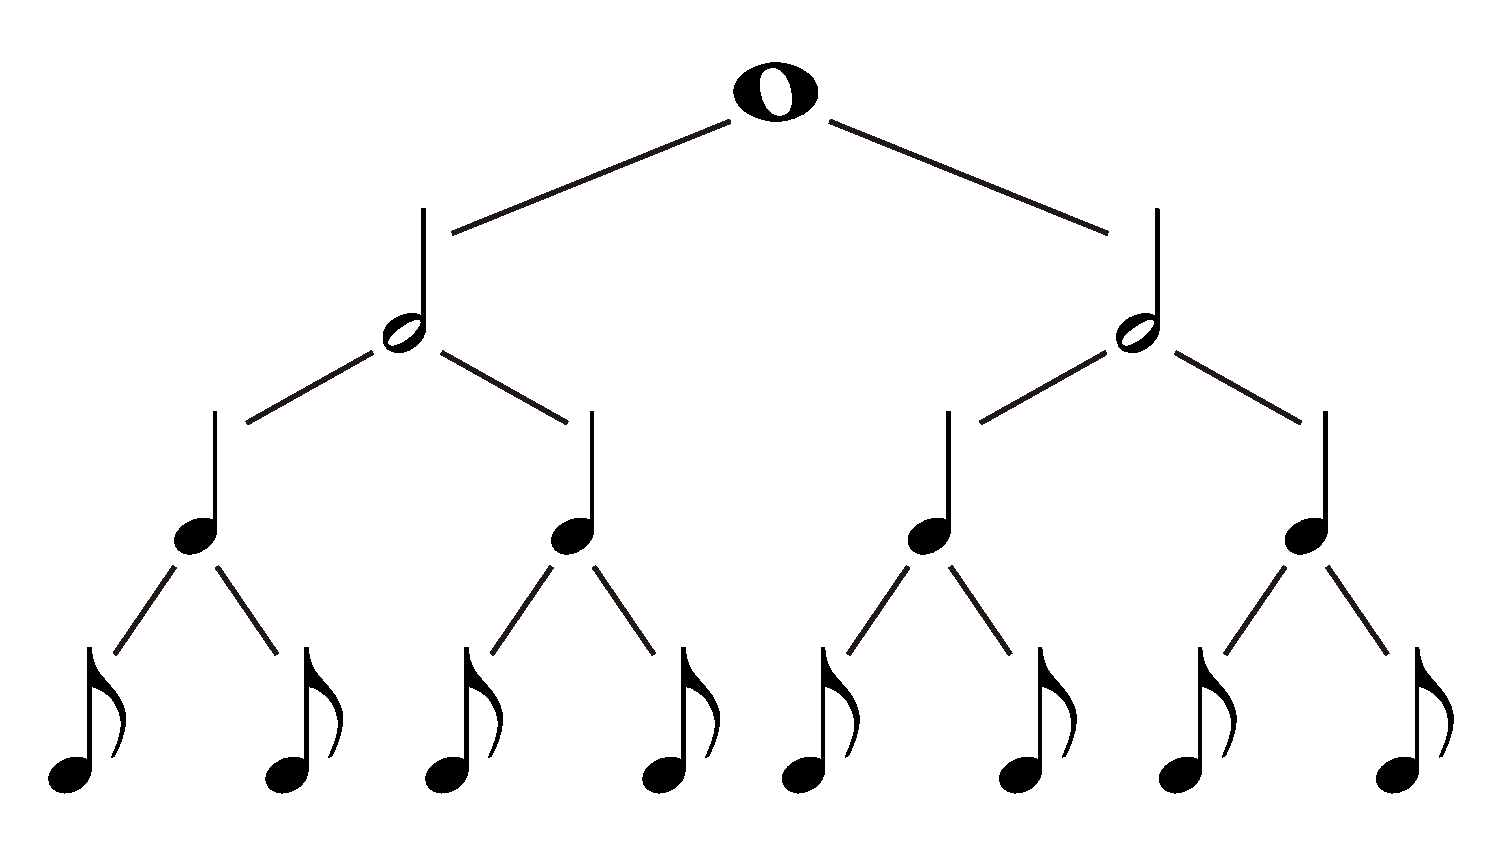
\includegraphics[width=0.8\linewidth]{imagenes/music_tree.pdf}
	\caption{Diagrama de subdivisión de figuras}
	\label{fig:subdivision-figuras}
\end{figure}

Dado que en inglés estas figuras se llaman mediante el nombre de la fracción de redonda que representan, también pueden ser representadas mediante el número del denominador de dicha fracción. De este modo la redonda sería 1, la blanca 2, la negra 4, la corchea 8, la semicorchea 16, etc. Adicionalmente existen modificadores de la duración de una figura como el puntillo, un pequeño punto situado a la derecha que alarga la duración en un 50\% más.

\begin{figure}[hp]
	\centering
	\begin{music}
		\largemusicsize
		\setlines1{1}
		\setclefsymbol1\empty
		\nobarnumbers
		\startextract                      % starting real score
		\Notes\wh i\hu i\qu i\cu i\en\bar
		\Notes\pause \hpause \qp \ds \en
		\setdoublebar\stoppiece
		\zendextract                       % terminate excerpt
	\end{music}
	\caption{Figuras con sus respectivos silencios, de izquierda a derecha: Redonda, blanca, negra, corchea}
	\label{fig:figuras}
\end{figure}

El \textit{tempo}, anteriormente mencionado, es una relación que indica la cantidad aproximada de figuras de negra que suenan en un minuto. Debido a eso la magnitud que representa el \textit{tempo} se denomina BPM o \textit{Blacks per Minute}.

La partitura está dividida en compases, y al principio de la pieza se indica el tipo de compás de la misma. Se representa con dos números colocados en vertical que indican respectivamente la cantidad de figuras que caben en cada compás y el tipo de dicha figura, utilizando el sistema del numerador de la fracción de redonda detallado anteriormente. A modo de aclaración, el tipo de figura utilizado en el compás solamente indica la figura base del mismo, pero eso no impide que se utilicen fracciones o figuras de mayor longitud equivalentes siempre y cuando se respete que la suma de sus duraciones no supere la especificada en el tipo de compás. 

Según la cantidad de figuras que caben en cada compás, estos reciben diferentes nombres. En la música moderna lo más habitual es encontrar compases binarios o cuaternarios, aunque en algunas corrientes de la música clásica como el \textit{Waltz} predominan los ternarios. 

\begin{figure}[hpt]
	\centering
	\begin{music}
		\largemusicsize
		\setlines1{1}
		\setclefsymbol1\empty
		\generalmeter{\meterfrac{4}{4}}%
		\nobarnumbers
		\startextract                      % starting real score
		\Notes\cu i\hu i\qu i\cu i\en
		\generalmeter{\meterfrac{3}{4}}\changecontext
		\Notes\qu i\hu i\en
		\setdoublebar\stoppiece
		\zendextract                       % terminate excerpt
	\end{music}
	\caption{Ejemplos de tipos de compases: Cuaternario y Ternario}
	\label{fig:compas}
\end{figure}

El acento en la música es un mero hincapié interpretativo en los tiempos fuertes de la pieza. Aunque puede existir una acentuación arbitraria a lo largo de la partitura, los compases determinan además los tiempos fuertes y normalmente acentuados. Dependiendo del tipo de compás estos varían, aunque la primera figura de cada compás suele estar acentuada y ser considerada fuerte. No obstante, la diferenciación de tiempos débiles y fuertes es importante en la melodía y por tanto en la armonía, por ello se revisará este concepto en los puntos siguientes.


\subsection{Melodía y pentagrama}
\label{subsec:melody_pentagram}
La melodía de la pieza es la secuencia temporal de notas que siguen las diferentes voces a lo largo de la partitura leyéndola horizontalmente. Para ello se utilizan siete notas fundamentales diferentes: Do, Re, Mi, Fa, Sol, La y Si (C, D, E, F, G, A, B en la notación internacional). Entre cada una de estas notas fundamentales se establece una distancia en frecuencia conocida como tono, excepto entre Si y Do; y entre Mi y Fa, entre las cuales sólo hay medio tono (también denominado semitono). Las fundamentales pueden ser alteradas mediante modificaciones conocidas como \textit{sostenido} y \textit{bemol}, que suben o bajan, respectivamente, un semitono a dichas notas. Por eso podemos entender que contamos, en total, con 12 sonidos distintos. Las alteraciones son muy fáciles de entender en las teclas del piano, ya que las notas sin alterar corresponden a las teclas blancas mientras que las alteradas corresponden a las negras que hay entre algunas de las blancas. 

\begin{figure}[h]
	\centering
	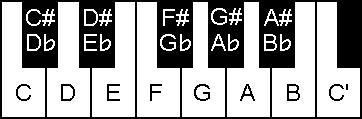
\includegraphics[width=0.5\linewidth]{imagenes/PianoKeys.png}
	\label{fig:paino-keys}
	\caption{Disposición de los doce sonidos disponibles en cada octava sobre las teclas del piano}
\end{figure}

Estas siete notas fundamentales (o doce sonidos), tienen asociadas a su vez una octava. Cada octava es un conjunto formado por esos mismos sonidos pero en un registro más agudo o más grave. Si bien esto produce un sonido diferente, el mismo sonido de diferentes octavas es, de modo general, equivalente en términos de armonía.

La representación de estos sonidos se hace sobre un pentagrama, bandas formadas por cinco líneas con sus respectivos cuatro huecos donde pueden colocarse las notas de la partitura, representando cada línea y hueco consecutivos una nota fundamental diferente. Ya que esto solo permitiría representar nueve notas, se pueden utilizar líneas y huecos adicionales situados encima y debajo del pentagrama para indicar notas más graves o más agudas. En conjunción con las alteraciones ya mencionadas (Sostenido y Bemol) en un mismo pentagrama pueden representarse más de una veintena de sonidos diferentes. 

Para poder interpretar el sonido correspondiente a cada línea o hueco existe la clave. La clave es un símbolo situado al principio de cada pentagrama e indica la nota correspondiente a una de las cinco líneas. El resto se calculan subiendo o bajando huecos y renglones a partir de esa línea. 

\begin{figure}[h!]
	\centering
	\begin{music}
		\largemusicsize
		\generalmeter{\meterfrac{4}{4}}%
		\nobarnumbers
		\startextract                      % starting real score
		\Notes\qu {abcd}\en
		\setclef1\bass\changecontext
		\Notes\qu {abcd}\en
		\setdoublebar\stoppiece
		\zendextract                       % terminate excerpt
	\end{music}
	\caption{La misma secuencia de notas en clave de Sol y de Fa}
	\label{fig:claves}
\end{figure}

En la Figura \ref{fig:claves}, la clave de Sol indica que en la segunda línea, contando desde abajo, estaría ubicada la nota sol, mientras que la clave de Fa\footnote{En este caso, la clave de ``Fa en 4ª'', ya que existen claves de ``Fa en 2ª'' y ``Fa en 3ª''} indica que en la cuarta línea, contando también desde abajo, se ubicaría el sonido Fa. La finalidad de las diferentes claves es ofrecer diferentes puntos de referencia, ya que no solo indican nota sino también octava, evitando así sobrecargar la partitura con notas fuera de las cinco líneas principales. La clave de Sol utiliza sonidos más agudos, mientras que la de Fa utiliza sonidos más graves. Es habitual encontrar, por ejemplo, partituras para piano donde la mano izquierda estará escrita en clave de Fa al ser notas más graves y en clave de Sol la de la mano derecha, al ser notas más agudas. 

Un salto melódico es la diferencia de frecuencia entre dos sonidos consecutivos de una misma melodía. De este modo, si el siguiente sonido es más agudo se producirá un salto ascendente, y si es más grave, descendente. Las secuencias ascendentes y descendentes se combinan con el ritmo de la canción para crear tramos de tensión melódica, de resolución, de reposo... Para entender estos conceptos es necesario introducir el concepto de escala. 

\begin{figure}[h!]
	\centering
	\begin{music}
		\largemusicsize
		\nobarnumbers
		\startextract                      % starting real score
		\Notes\cu {cdefghij}\en
		\setdoublebar\stoppiece
		\zendextract                       % terminate excerpt
	\end{music}
	\begin{music}
		\largemusicsize
		\nobarnumbers
		\startextract                      % starting real score
		\Notes\cu {cd_efg_h_ij}\en
		\setdoublebar\stoppiece
		\zendextract                       % terminate excerpt
	\end{music}
	\label{fig:escalas}
	\caption{Escalas de Do Mayor y Do Menor}
\end{figure}

Una escala es un subconjunto de los doce sonidos disponibles donde sus miembros cumplen una distribución concreta de separaciones tonales. La escala más conocida es la de Do Mayor, ya que empezando desde Do, pasa por las siete notas fundamentales sin alterar (ver \ref{fig:escalas}). Si se mira de desde la distribución de tonos y semitonos entre las notas de Do Mayor (Tono, Tono, Semitono, Tono, Tono, Tono, Semitono) se puede construir cualquier otra escala mayor dada una nota arbitraria de partida. Las escalas pueden ser, según su distribución tonal Mayores o Menores, así como recibir diferentes nombres según la cantidad de sonidos que incluyan. La escala sobre la que se construye una pieza puede ser denominada tonalidad y recibe el nombre de la nota raíz junto con su modo. Así una pieza construida con la escala de Do Mayor puede decirse que está en tonalidad de Do Mayor.

En aquellas piezas en las que se trabaja con una determinada tonalidad hay una serie de notas que deben aparecer siempre alteradas. En esos casos resulta cómodo especificar una \textit{armadura}. La armadura es un conjunto de alteraciones al principio del pentagrama, justo a la derecha de la clave, que indica qué alteraciones tendrán las notas de ese pentagrama a lo largo de toda la canción o hasta que se especifique lo contrario. De este modo, para la escala de Do Menor de la Figura \ref{fig:escalas} podría especificarse una armadura que indicase tres bemoles en las líneas de mi, la y si. Si quisiéramos escribir esas notas sin la alteración, para contrarrestar la armadura, habría que usar otra alteración denominada \textit{becuadro}. El becuadro, también conocido como \textit{natural}, elimina las alteraciones establecidas por la armadura del pentagrama. Esta armadura no solo resulta conveniente para el compositor, al tener que escribir las alteraciones de las notas una única vez al comienzo, sino que también es muy útil a la hora de identificar la tonalidad de la pieza, ya que suele ser un indicativo fiable de la misma.

\begin{figure}[h]
	\centering
	\begin{music}
		\largemusicsize
		\nobarnumbers
		\startextract                      % starting real score
		\Notes\cu {cd_efg_h_ij}\en
		\setdoublebar\stoppiece
		\zendextract                       % terminate excerpt
	\end{music}
	\begin{music}
		\largemusicsize
		\nobarnumbers
		\setsign1{-3}
		\startextract                      % starting real score
		\Notes\cu {cdefghij}\en
		\setdoublebar\stoppiece
		\zendextract                       % terminate excerpt
	\end{music}
	\caption{Escala de Do Menor sin armadura y con armadura}
	\label{fig:armadura}
\end{figure}

\subsection{Armonía}
\label{subsec:harmony}
Si la melodía es la sucesión de notas en el tiempo, se puede entender la armonía como los conjuntos de notas que suenan a la vez a lo largo de un intervalo de tiempo. Por eso se habla de que el análisis melódico es horizontal y el armónico vertical, aunque esto no es del todo cierto, pues al fin y al cabo la armonía analiza también intervalos horizontales de tiempo (normalmente acotados en compases) y la estructura general de la pieza. Para poder estudiar o crear armonía se debe contar siempre, o bien con varias voces, o bien con instrumentos polifónicos capaces de producir sonidos simultáneos (Como el Piano o la Guitarra).

Uno de los conceptos más importantes dentro de la armonía es la tonalidad. La armonía define siete grados para una tonalidad, y están relacionados con la escala de dicha tonalidad. Cada grado está referido a cada una de las notas de la escala y se representa mediante un número romano de forma consecutiva, además de un nombre. Los grados más relevantes son el I, IV y V, mientras que los menos importantes o débiles son el II y el VI. A mayores, los grados muy débiles son el III y el VII.

\begin{itemize} 
	\item I (Tónica)
	\item II (Supertónica)
	\item III (Mediante)
	\item IV (Subdominante)
	\item V (Dominante)
	\item VI (Superdominante/Submediante)
	\item VII (Sensible)
\end{itemize}

Establecidos los grados podemos comprender el concepto de intervalo entre dos notas. Dados los grados de dos notas cualesquiera, contando los grados intermedios entre ambas podemos determinar el intervalo. De este modo existiría un intervalo de segunda entre el grado I y el grado II, un intervalo de tercera entre el grado II y el grado IV, un intervalo de cuarta entre el grado III y el grado VI, etc. Este intervalo puede ser ascendente o descendente si la segunda nota del intervalo es más aguda que la primera o más grave.

Según la teoría, un acorde son tres o más sonidos simultáneos a una distancia de tercera entre sí de forma ascendente. Analizando el tercer grado de la escala de las notas del acorde, podemos determinar si éste es mayor o menor. La nota generadora del acorde suele ser la tónica y además la más grave del mismo, si no es así se dice que el acorde está invertido.

\begin{figure}[h!]
	\centering
	\begin{music}
		\largemusicsize
		\nobarnumbers
		\startextract                      % starting real score
		\Notes\zq{ce}\qu g\en
		\Notes\zq{df}\qu h\en
		\Notes\zq{eg}\qu i\en
		\Notes\zq{fh}\qu j\en
		\Notes\zq{gi}\qu k\en
		\Notes\zq{hj}\qu l\en
		\Notes\zq{ik}\qu m\en
		\setdoublebar\stoppiece
		\zendextract                       % terminate excerpt
	\end{music}
	\caption{Acordes de la tonalidad de Do Mayor}
	\label{fig:acordes}
\end{figure}


Ciertas combinaciones de acordes producen sensación de tensión, mientras que otras producen sensación de reposo. Algunos acordes, según el contexto, tienen un sentido conclusivo y otros, un sentido transitorio. Estos conceptos son muy importantes en composición, así como en armonización.

La armonización es el proceso de construir una armonía mediante varias voces que, sin modificar la melodía de la pieza, enriquezca la misma reforzando la tonalidad en cada instante. Esto se consigue identificando la tonalidad de la pieza en cada tramo, tomando las notas del mismo y averiguando la escala sobre la que se ha construido la melodía. Dada la escala podemos identificar la tonalidad, y con la tonalidad construir por fin los acordes. 

\begin{figure}[h]
	\centering
	\begin{music}\nostartrule
		\parindent10mm
		\nobarnumbers
		\instrumentnumber{1}       % a single instrument
		\setname1{Piano}           % whose name is Piano
		\setstaffs1{2}             % with two staffs
		\generalmeter{\meterfrac44}% 4/4 meter chosen
		\startextract              % starting real score
		\Notes\ibu0f0\qb0{cge}\tbu0\qb0g|\hl j\en
		\Notes\ibu0f0\qb0{cge}\tbu0\qb0g|\ql l\sk\ql n\en
		\bar
		\Notes\ibu0f0\qb0{dgf}|\qlp i\en
		\notes\tbu0\qb0g|\ibbl1j3\qb1j\tbl1\qb1k\en
		\Notes\ibu0f0\qb0{cge}\tbu0\qb0g|\hl j\en
		\setdoublebar\stoppiece
		\zendextract                 % terminate excerpt
	\end{music}
	\caption{Ejemplo de polifonía para Piano (Sonata en Do Mayor, Mozart)}
	\label{fig:polifonia}
\end{figure}

No obstante, existen reglas a respetar, ya que no es tan sencillo como tomar cada nota de la melodía como nota generadora de un acorde y construir el acorde mayor o menor correspondiente a la misma. Por otra parte no basta con tocar el acorde principal de la tonalidad a lo largo de toda la pieza, ya que si bien esto no sería erróneo, en algunos casos podría producir problemas con las fluctuaciones de la melodía, y no cumpliría, en último extremo, la finalidad de enriquecer la melodía.

Los acordes no solo deben respetar la melodía, sino que además deben ser escogidos de tal forma que se enlacen correctamente, normalmente debido a las notas compartidas entre dos acordes consecutivos. Las notas distintas al enlazar dos acordes pueden producir sonidos indeseados con respecto a la melodía o causar saltos melódicos no agradables al oído. Para evitar estos problemas se estudia a su vez, horizontalmente, las nuevas líneas melódicas formadas por las diferentes voces de los acordes. Los diferentes movimientos de estas voces podrían ser, entre otros:

\begin{itemize} 
	\item Paralelo: Dos voces de varios acordes siguiendo una distancia, realizando los mismos saltos melódicos.
	\item Oblicuo: Una voz representada con una nota de larga duración y otra voz moviéndose libremente.
	\item Directo: Dos voces moviéndose a la vez de forma ascendente o descendente, pero no en paralelo.
	\item Contrario: Dos voces moviéndose en sentidos opuestos.
\end{itemize}

En movimientos como el paralelo o el contrario pueden surgir problemas armónicos, como formar un intervalo de octava o quinta justa sobre las mismas voces. El movimiento directo también presenta problemas armónicos, en voces extremas (Bajo y Soprano), si la voz de la Soprano (más aguda) no se mueve por determinados grados, se presenta ese problema. En partes intermedias (voces centrales o una voz central y otra extrema), si una de esas dos voces no se mueve por grados conjuntos, ese enlace sería incorrecto. En voces seguidas, se busca evitar los saltos de octava.

\subsection{Modulación}
\label{subsec:modulation}
La modulación es el cambio de tonalidad a lo largo de una partitura. Normalmente ésta viene indicada por un cambio de armadura en la sección en la que se produce el cambio, pero no siempre es así y, a veces, si el tramo no es lo suficiente extenso o se pretende alcanzar una tonalidad más alejada armónicamente de la que se está utilizando en la partitura, puede realizarse modulación mediante alteraciones en las notas de la partitura sin indicarla en la armadura por no dificultar la lectura de la misma.

\subsection{Tesitura}
\label{subsec:tessitura}
La tesitura define el rango de notas que un instrumento o tipo de voz es capaz de alcanzar, siendo el límite inferior la nota más grave que puede producir y el superior la más aguda. Referido a la voz humana, a veces no se refiere tanto a los límites de las frecuencias sonoras que puede alcanzar sino a aquel rango en el que la voz logra una mejor calidad. Es por esto que a veces un mismo cantante puede cantar diferentes partes de la pieza asignadas a tesituras diferentes si fuera necesario.

En música coral se diferencian las tesituras por el sexo\footnote{Existen excepciones como los coros en que las tesituras femeninas son interpretadas por niños o en algunos casos por los conocidos como ``castrati'', varones que eran castrados en la infancia para mantener su timbre agudo.} de la persona que canta y se les asignan roles en la polifonía del mismo modo que se asignan a los diferentes instrumentos en una orquesta. Las tesituras corales más comunes son:

\begin{itemize}
	\item Bajo: Voz masculina encargada de las partes más graves
	\item Barítono: Voz masculina intermedia
	\item Tenor: Voz masculina más aguda
	\item Contra-Tenor: Voz masculina especialmente aguda, normalmente cantada en falsete
	\item Contralto: Voz femenina más grave, no obstante, situada por encima de la de Contra-Tenor
	\item Mezzo-Soprano: Voz femenina intermedia entre la de Contralto y Soprano
	\item Soprano: Voz femenina encargada de las secciones más agudas
\end{itemize} 

\section{Contexto Tecnológico}
\label{sec:contexto-tecnologico}

\lettrine{L}a mayor parte del trabajo en la creación y composición musical en ordenadores se ha extraído de la relación entre la teoría musical y las matemáticas. No es difícil concluir que la música y sus reglas son fácilmente modelables de forma matemática. 

Dentro de la música en computación existen varias ramas diferenciadas, aunque en el contexto de un mismo trabajo pueden verse mezcladas más de una. Hablamos de composición asistida y de de sistemas inteligentes orientados a composición y, aunque se tratarán con más detalle en los siguientes puntos, todos ellos, así como el software desarrollado en dichos campos, están destinados a la creación y composición musical. Se detallan, además, algunos de los formatos más comunes de representación musical.

Si bien el sistema planteado en el proyecto no es un compositor, se enmarca dentro de este mismo contexto, y por tanto es necesario desglosarlo para entender en qué punto se encuentra la tecnología desarrollada en el momento de la publicación de este documento.

\subsection{Answer Set Programming}
\label{subsec:asp}
El módulo principal del proyecto se ha desarrollado usando técnicas conocidas como \textit{Answer Set Programming}\cite{Brewka:2011:ASP:2043174.2043195} (ASP de ahora en adelante) basadas en modelos estables (Gelfond \& Lifschitz 1988) y lógica no-monótona. ASP es un lenguaje de programación declarativa orientado a problemas de búsqueda difíciles, principalmente NP-complejos. ASP ha demostrado ser particularmente útil en aplicaciones donde es necesaria la representación del conocimiento y el razonamiento a partir de dicho conocimiento. En ASP, los problemas de búsqueda se reducen al cómputo de modelos estables, usándose programas conocidos como\textit{solvers} para realizar la búsqueda de las soluciones. El lenguaje de entrada de ASP es una variante enriquecida del lenguaje prolog. Para traducir el lenguaje de entrada a reglas de programación declarativa convencional y poder construir los modelos estables subyacentes del problema, ASP cuenta con \textit{grounders} que se encargan de esta transformación.

La implementación de un programa que busque soluciones a un problema concreto pasa por la definición de las reglas de ese problema de modo general, mientras que la definición del problema concreto a solucionar se especifica mediante hechos lógicos que, en combinación con las reglas generales del problema generan todas las posibles soluciones del mismo. Finalmente, estas soluciones se podan mediante restricciones lógicas y/o restricciones de cardinalidad. Este proceso constituye la metodología general del desarrollo en ASP, conocida como \textit{generate and test}

Las herramientas desarrolladas por el grupo Potassco\footnote{http://potassco.sourceforge.net/} incluyen, entre otras, un \textit{grounder} (Gringo) y un \textit{solver} (Clasp), junto con una herramienta única que combina ambos llamada Clingo.

\begin{itemize}
 \item \textbf{Gringo} es el \textit{grounder} de la suite. Se encarga de transformar reglas generales a reglas concretas y transforma el problema planteado a un lenguaje entendible por el \textit{solver}
 
 \item \textbf{Clasp} es el \textit{solver} de la suite. Se encarga de decidir el conjunto final de soluciones válidas dado el problema procesado e interpretado por el \textit{grounder}
 
 \item \textbf{Clingo} es una herramienta combinada formada por clasp y gringo. Realiza el procesado completo de un problema planteado en ASP y permite indicar algunas preferencias adicionales
\end{itemize}

\subsection{Formatos}
\label{subsec:formats}
Debido al contexto en el que se enmarca este proyecto no se cree necesario considerar formatos de salida finales, como OGG, WAV o MP3 ya que como su nombre indica, son formatos utilizados solo para reproducción que no permiten extraer ni editar información musical de forma precisa. Así mismo tampoco se contemplan formatos de representación de partituras en forma de imágenes como SVG, PNG o PDF por motivos similares.

\subsubsection{MusicXML}
MusicXML, MXML o \textit{Music Extensible Markup Language} es una extensión del formato XML usado en la representación de música occidental. No solo contiene información musical sino que también incluye información de su representación en papel, tal como márgenes, tamaños de fuente, posición de las notas en coordenadas, etc. Hace uso del sistema de etiquetas anidadas de XML para agrupar los diferentes bloques de información de una pieza, como las voces, los compases o la información individual de cada nota. Es un formato muy rico aunque difícil de escribir correctamente a mano. Es por esto que normalmente se usa solo como formato de intercambio entre software que lo acepta como entrada o salida.

\begin{figure}[h!]
	\centering
	\begin{verbatim}
	<note default-x="74.65" default-y="-25.00">
	    <pitch>
	        <step>A</step>
	        <octave>4</octave>
	    </pitch>
	    <duration>1</duration>
	    <voice>1</voice>
	    <type>quarter</type>
	    <stem>up</stem>
	</note>
	\end{verbatim}
	\caption{Ejemplo de nota representada en MusicXML}
	\label{fig:nota_musicxml}
\end{figure}


\subsubsection{LilyPond}
LilyPond\footnote{http://www.lilypond.org/} es un conjunto formado por el software y el formato de fichero homónimos. LilyPond como formato usa su propio lenguaje de marcado. Las eqtiquetas de LilyPond se parecen más a las usadas en \LaTeX. De forma similar a MusicXML, incluye información de representación final, aunque en mucha menor cantidad (Sólo tamaño de papel, márgenes o sangrados). La información musical de la canción está anidada por secciones de forma similar a MusicXML, aunque ésta se organiza de forma mucho más intuitiva para el lector humano del fichero. Es un formato ligero pensado para poder ser editado a mano, aunque la mayoría del software musical actual lo soporta como entrada y salida. 

El software del mismo nombre es un programa de grabado musical (tipografía musical o edición de partituras), pensado para producir partituras de alta calidad. Lleva la estética de la música tipografiada de la forma tradicional a las partituras impresas mediante ordenador. LilyPond es software libre y forma parte del Proyecto GNU. 

\begin{figure}[h!]
	\centering
	\begin{verbatim}
		\version "2.14.1"
		{
		  <c' d'' b''>8. ~ <c' d'' b''>8
		}
	\end{verbatim}
	\caption{Ejemplo de una pequeña pieza musical en lilypond}
	\label{fig:partitura_lilypond}
\end{figure}



\subsubsection{MIDI}
MIDI son las siglas de \textit{Musical Instrument Digital Interface}. Es un standard técnico compuesto de un protocolo, una interfaz digital y conectores que permiten a una gran variedad de instrumentos electrónicos, ordenadores y otros dispositivos conectarse y comunicarse entre sí, principalmente con fines musicales, pero no siempre.

MIDI transmite mensajes de eventos que especifican notación, tono y velocidad, aunque también incluye información de modificaciones sobre estos sonidos como volumen, \textit{vibrato} y marcas de tiempo para sincronizar entre dispositivos. 

Estos mensajes pueden ser codificados en ficheros para reproducción, edición o simplemente como formato de representación musical pudiendo ser editado posteriormente. Dado que no contiene información final de audio, MIDI supone una gran ventaja en cuanto a espacio en disco, aunque el sonido final depende del equipo que reproduzca el fichero.


\subsection{Software}
\label{subsec:software}
\subsubsection{Herramientas}
\begin{itemize}
	\item \textbf{Flex y Bison} son utilidades Unix que permiten escribir \textit{parsers} veloces para casi cualquier formato de archivo. Implementan procesado \textit{Look-Ahead-Left-Right} de gramáticas libres de contexto no ambiguas.
	\item \textbf{Music21} es un conjunto de herramientas que sirve de ayuda a estudiantes y músicos a responder preguntas sobre música rápida y eficazmente. No sólo posee una base de datos bastante completa para realizar análisis musicológicos sino que contiene herramientas para la composición programática de música.
\end{itemize}

\subsubsection{Composición Asistida}
Dentro de la composición asistida encontramos principalmente software de composición general en forma de editores de partituras que incorporan herramientas para ayudar al compositor en el proceso. Estas herramientas pueden ser corrección de la métrica de los compases, transposición de secciones de la canción, cambios de tonalidad, construcción de acordes dada una nota generadora, etc.

\begin{itemize}
 \item \textbf{Musescore 2} es un editor \textit{WYSIWYG} capaz de exportar a varios formatos de representación musical digital, tales como MIDI, LilyPond o MusicXML.
\item \textbf{Sibelius} permite trabajar con gran variedad de modos de entrada de notas para sus partituras, desde los formatos convencionales hasta a través de instrumentos con salida MIDI o mediante el escaneado de partituras en papel haciendo uso de OCR.
\item \textbf{Finale} destaca por la cantidad de ajustes que permite realizar sobre el pentagrama a un nivel de detalle muy fino, aunque presenta una curva de aprendizaje muy elevada. Sus principales características  tienen que ver con la visualización del pentagrama, ya que posee \textit{plug-ins} que se encargan de que el espacio entre las notas sea el correcto o que no haya colisiones entre notas de diferentes voces entre otros. 
\end{itemize}


\subsubsection{Sistemas Inteligentes}
Aunque la música puede modelarse de forma matemática, con reglas estrictas que derivan en algoritmos de composición, también requiere creatividad. Un algoritmo determinista no puede ser creativo, ya que para la misma entrada, siempre producirá la misma salida. Si bien existe la composición algorítmica como aproximación a la música compuesta por ordenadores, no es relevante para este trabajo.

Dentro de la inteligencia artificial, se han realizado aproximaciones a la composición musical desde gran parte de las ramas principales del campo

\begin{itemize}
	\item \textbf{EMI y Emily Howell} Desarrollado por David Cope\cite{experiments-musical-intelligence}, EMI o Experiments in Music Composition, es un sistema capaz de identificar el estilo presente en una partitura incompleta y completar la cantidad de notas restantes que el compositor requiera. El trabajo de Cope estudia la posibilidad de emplear gramáticas y diccionarios en la composición musical. EMI derivó en el software Emily Howell.
	Emily Howell utiliza EMI para crear y actualizar su base de datos, pero cuenta con una interfaz a través de la cual se puede modificar, a través de \textit{feedback}, la composición. Cope enriqueció y pulió Emily Howell con su propio estilo musical para crear varios discos que después fueron publicados.
	\item \textbf{ANTON}\cite{anton-composing} es un sistema de composición rítmica, melódica y armónica basado en Answer Set Programming. ANTON compone breves piezas musicales desde cero o partiendo de partituras incompletas utilizando un estilo basado en el del compositor renacentista Giovanni Pierluigi da Palestrina. Recibe como entrada ficheros con las notas codificadas como hechos lógicos para después rellenar las secciones incompletas o añadir nuevas notas hasta que la pieza está completa. ANTON crea y completa dichas piezas teniendo en cuenta el número de tiempos rítmicos de las mismas y seleccionando la nota correspondiente de acuerdo a la nota  o estado anterior.
	\item \textbf{Vox Populi}\cite{vox-populi} utiliza algoritmos evolutivos para componer música en tiempo real. En este sistema, se parte de una población de acordes codificados mediante el protocolo MIDI para después mutarlos y seleccionar los mejores acordes a criterios puramente físicos relevantes para la música. Su interfaz gráfica permite al usuario controlar la función de \textit{fitness} del proceso evolutivo así como los atributos del sonido producido.
	\item \textbf{CHORAL} es un sistema experto que funciona como armonizador en el estilo clásico de Johann Sebastian Bach. Las reglas que utiliza el sistema representan conocimiento musical desde varios puntos de vista de la coral. El programa armoniza melodías corales mediante un sistema de generación y prueba con \textit{backtracking}. La base de conocimiento de CHORAL permite realizar modulaciones propias del estilo, crear patrones rítmicos e impone restricciones complejas para mantener el interés melódico en las voces intermedias.
	\item \textbf{CHASP} es una herramienta creada por el grupo Potassco para calcular progresiones de acordes mediante Answer Set Programming partiendo de cero, pudiendo especificar clave y duración. A diferencia del presente proyecto no toma un fichero de entrada para armonizar piezas, pero sí que es capaz de dotar a la salida del programa de diferentes estilos rítimicos.
\end{itemize} 





 \chapter{Trabajo Desarrollado}
\label{chap:desarrollo}
\vspace{0.5cm}

%%%%%%%%%%%%%%%%%%%%%%%%%%%%%%%%%%%%%%%%%%%%%%%%%%%%%%%%%%%%%%%%%%%%%%%%%%%%%%%%
% Objetivo: Exponer las partes relevantes de la implementación                 %
%%%%%%%%%%%%%%%%%%%%%%%%%%%%%%%%%%%%%%%%%%%%%%%%%%%%%%%%%%%%%%%%%%%%%%%%%%%%%%%%

\section{Metodología}
\label{sec:metodology}
\lettrine{E}{s} difícil hablar de una planificación del proyecto como tal ya que por sus particularidades se han amalgamado características de varias metodologías. Lo que sí está claro es que el proyecto ha seguido una metodología ágil debido a su carácter de desarrollo evolutivo y orientado a la creación de prototipos funcionales en cada iteración. Se podría considerar que está a medio camino entre SCRUM y un ciclo de desarrollo en espiral con prototipado, ya que ha sido un proceso iterativo. Sin embargo, no es correcto decir que se ha utilizado SCRUM como metodología al no ser fácil repartir las tareas de cada iteración ni tener con quién hacerlo por ser un trabajo desarrollado por un único alumno junto con su director. 

La similaridad con el ciclo de desarrollo en espiral reside en que en cada iteración se pasan por los mismo puntos, revisando y modificando cada uno de los componentes para llegar al prototipo objetivo. Tras el trabajo, dicho prototipo es revisado en la reunión con el ``cliente'', que en este caso es el director del proyecto, revisando la funcionalidad implementada y dirigiendo los siguientes pasos.

Pese a las dificultades, disponiendo de una agenda de producto similar a la de SCRUM a modo de requisitos, se han podido trazar una serie de iteraciones. Cada iteración cuenta con su agenda de iteración en la cual se detallan los requisitos del prototipo a crear en ese paso haciendo evolucionar cada uno de los componentes. Se habla de hacer evolucionar los componentes y no de incrementarlos porque, pese a que cada iteración ha procurado incrementar la funcionalidad total del sistema, algunos módulos del mismo han sido refactorizados\footnote{Es decir, se ha cambiado su diseño, sin alterar su propósito funcional} en determinados pasos.

En cuanto a la planificación de pruebas del sistema, si bien se ha contado con diferentes entradas con las que probar cada uno de los módulos que se han ido desarrollando junto con el proyecto, no se puede decir que el desarrollo de una herramienta de estas características pueda ser dirigido por la prueba, ya que las soluciones halladas mediante \textit{Answer Set Programming} no pueden ser establecidas de antemano debido a su carácter no determinitsa.

Se estableció que la duración de cada iteración sería, en promedio, de semana y media. Esto equivale a unas 40 horas de trabajo por iteración, aunque se decidió permitir la flexibilización de las iteraciones ante imprevistos en el desarrollo. Esto no se corresponde con una metodología SCRUM típica en la que habría que desplazar tareas a las siguientes iteraciones, pero al ser solo una persona encargada de todo el trabajo, se decidió dotar a la metodología de cierta flexibilidad para no arrastrar trabajo. No obstante, esta flexibilización permite también ganar tiempo, ya que de completarse el trabajo antes de lo previsto se podría acortar el tiempo dedicado a alguna iteración.

Gracias a esta flexibilidad se logró depender solo de completar los objetivos de las diferentes agendas, logrando así independencia del factor tiempo, que ya venía fijado por los plazos de entrega propios del proyecto. 

\section{Planificación}
\label{sec:planning}
Debido a estos factores derivados de lo particular de desarrollar un sistema basado en \textit{Answer Set Programming}, se carece de una planificación inicial cerrada y completa que marque el tiempo estimado para cada una de las tareas en forma del tradicional diagrama de Gantt. No obstante, a modo de registro, sí se ofrece un diagrama similar que muestra el tiempo invertido en cada una de las iteraciones (Figura \ref{fig:tareas}).

\begin{figure}
	\centering
	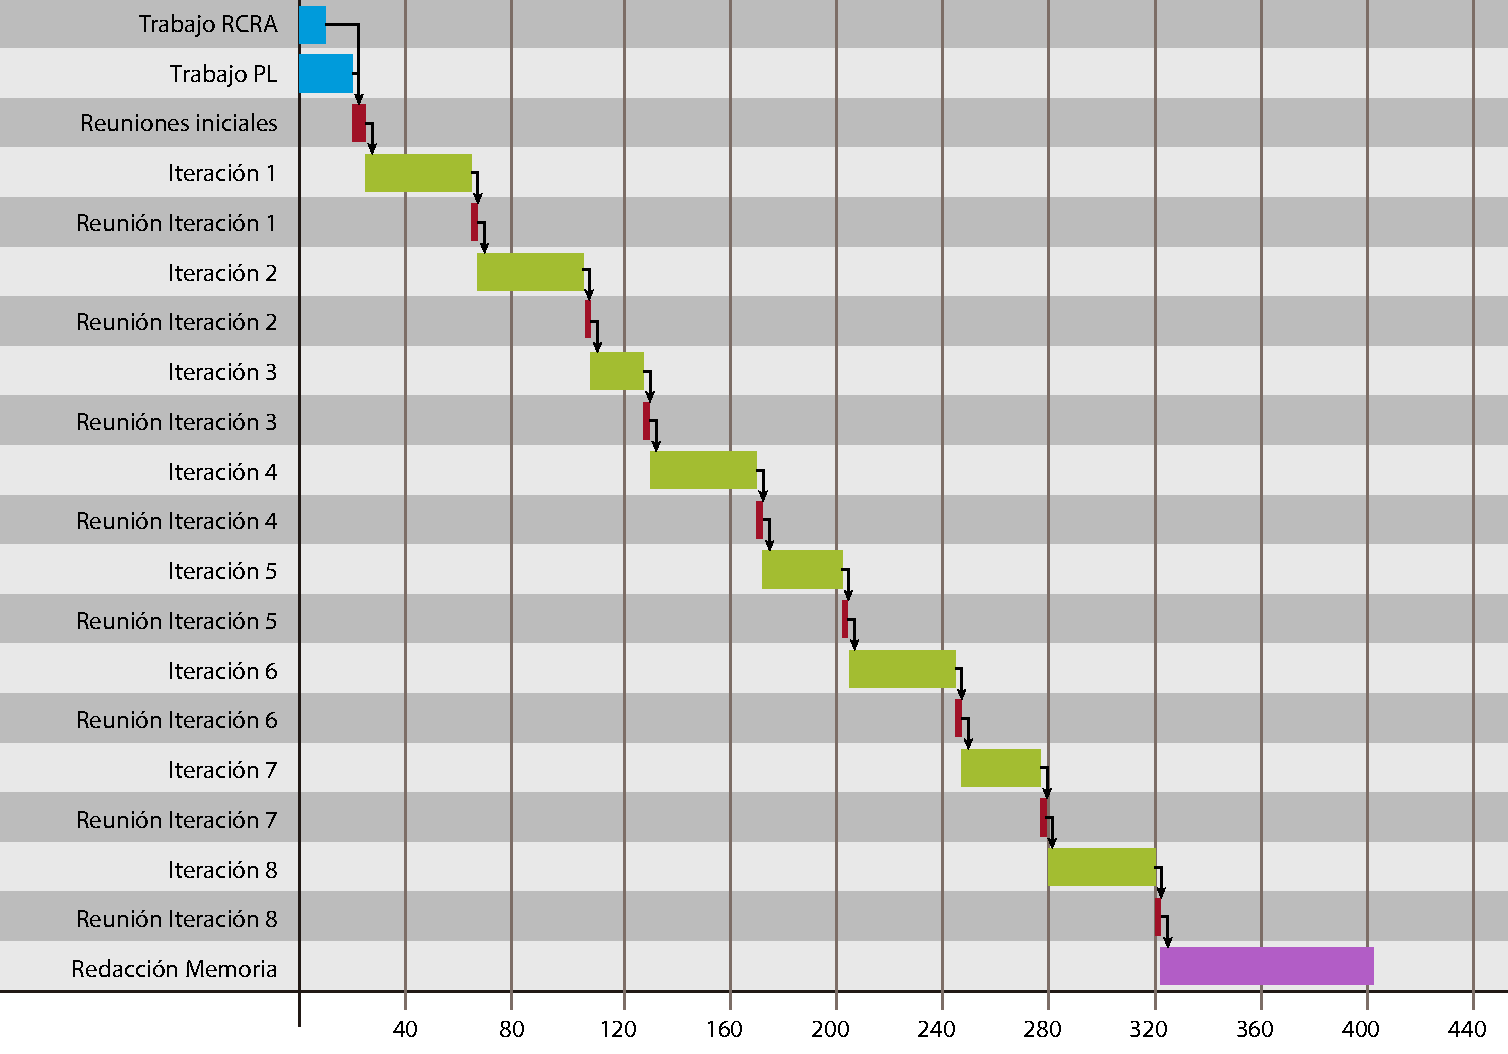
\includegraphics[width=0.8\linewidth]{imagenes/diagrama_tareas.pdf}
	\caption{Diagrama que muestra la secuencia de tareas}
	\label{fig:tareas}
\end{figure}

Dado este diagrama, es relativamente sencillo realizar una primera estimación del coste del proyecto. Hay que tener en cuenta, no obstante, horas extra de desarrollo que se incluyen en el diagrama y en el presupuesto ya que el trabajo no empezó de cero, al haberse realizado dos prácticas durante los años tres y cuatro del grado que se han reutilizado en menor o mayor medida para comenzar el desarrollo del presente trabajo. En la asignatura de ``Representación del Conocimiento y Razonamiento Automático'' se desarrolló una pequeña herramienta en \textit{Answer Programming} capaz de completar y componer pequeñas piezas musicales en forma de \textit{Canon}, mientras que en la asignatura de ``Procesamiento de Lenguajes'' se creó una primera versión del procesador de MusicXML a hechos lógicos. Se ha realizado una estimación de que, de no haber trabajado en la práctica de RCRA, se habrían necesitado unas 10 horas adicionales en los primeros pasos del desarrollo del módulo de armonización de este proyecto, mientras que de no haber realizado la práctica de PL se habrían necesitado unas 20 horas adicionales.

Sumado a 40 horas por iteración y contando con 8 iteraciones, arrojan un total de 350 horas de desarrollo. Las reuniones de final de iteración duraron una hora escasa cada una, pero al haber habido más de una por iteración y que las primeras reuniones fueron más extensas al tener que definir y planificar el proyecto se estima que el proyecto contó con unas 12 horas de reuniones para las que hay que sumar el coste por hora del tiempo del director.

Se ha asignado un coste aproximado de hora de trabajo del proyectando de 5.5\euro{}/hora y un coste también aproximado de 9\euro{}/hora para el director del proyecto. Con un cálculo rápido el coste del proyecto suma 1925\euro{} por las horas de desarrollo, 66\euro{} por las horas de reuniones por parte del alumno y 108\euro{} por las horas de reuniones por parte del director, haciendo un total de \textbf{2099\euro{}} para el diseño y desarrollo completo del mismo.

El coste de producción del proyecto es esencialmente el mismo que el de desarrollo, ya que las licencias de todo el software utilizado son gratuitas y no requiere ningún tipo de hardware adicional para funcionar. Incluso el editor de partituras que se recomienda utilizar junto con el programa (MuseScore2) es libre y de código abierto.

\section{Desarrollo}
\label{sec:development}
La arquitectura de haspie es un sencillo pipeline escrito en Python con un único camino que se ejecuta siempre que se llama a la herramienta, este pipeline se encarga de llamar a cada uno de los submódulos, enmascarando así el comportamiento interno de cada uno de ellos. Este pipeline además permite en su llamada a través de línea de comandos especificar diferentes opciones que se pasan después a cada submódulo de forma individual, estas opciones pueden verse en detalle en el anexo \ref{chap:usage}.

\begin{figure}[h]
	\centering
	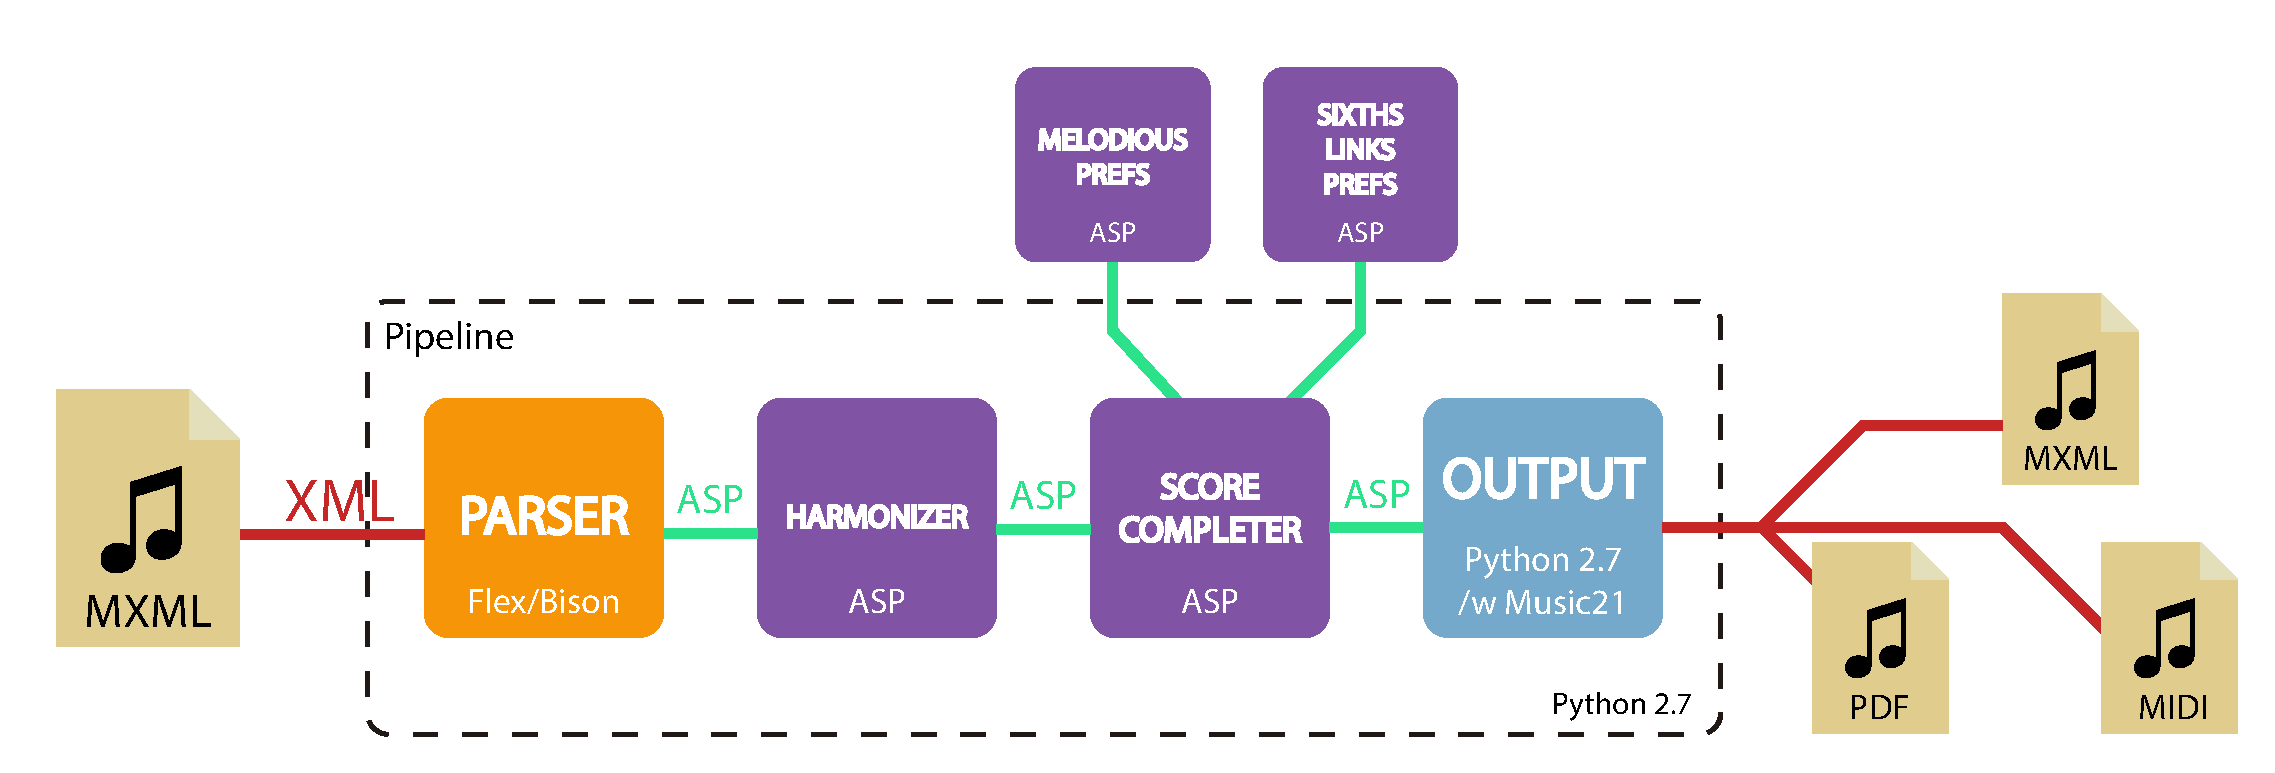
\includegraphics[width=0.8\linewidth]{imagenes/arquitectura_final.pdf}
	\caption{Arquitectura del sistema}
	\label{fig:arquitectura_final}
\end{figure}

\subsection{Entrada}
La entrada del sistema se realiza en formato MusicXML y el pipeline pasa la ruta del archivo especificado al módulo de entrada: un \textit{parser} escrito en C junto con las librerías Flex y Bison que se encarga de transformar los elementos de la partitura a hechos lógicos en Answer Set Programming. Este conversor no solo traduce las figuras y silencios a hechos sino que además:
\begin{itemize}
 	\item Subdivide todas las figuras de la partitura a la duración de la nota más breve de la pieza. Esta división es necesaria para que los módulos ASP puedan encajar correctamente todos los sonidos que se producen en cada tiempo de las diferentes voces de la pieza
 	\item Crea hechos lógicos adicionales \texttt{figure} que indican la duración original de cada una de las figuras con el fin de conservar esta información para que la pieza pueda ser reconstruida tras su procesado.
 	\item Itendifica las definiciones de la métrica de los compases que aparecen a lo largo de la partitura y convertirlos a los hechos lógicos correspondientes de modo que se pueda identificar correctamente el tipo de subdivisión de la partitura
 	\item Interpreta los nombres de los diferentes instrumentos de cada parte de la pieza y asigna hechos que vinculan cada una de las voces a un nombre instrumento o tipo de voz para poder detectar su tesitura
 	\item Lee la armadura de la partitura y determina la tonalidad y modo más probables correspondientes a la misma
 	\item Detecta el nombre y el autor de la partitura para poder representarlos en la salida
\end{itemize}
Aquellos datos procesados que no se convierten en hechos lógicos y se añaden al fichero ASP que servirá de entrada al núcleo dle programa se anotan en un fichero de configuración temporal que sirve a los distintos módulos del sistema para su funcionamiento.

El \textit{parser} funciona de un modo convencional, identificando las etiquetas relevantes que contienen la información necesaria para crear los hechos lógicos y almacenándolos en tipos de datos propio que se corrersponden con los elementos de la partitura tales como tipos de compás, anotaciones de acordes, nombres de instrumentos, nuevas voces, notas o silencios. A su vez, estos datos se almacenan en diferentes estructuras de cola (una para cada tipo de dato) mientras que se va procesando toda la pieza para calcular la longitud de la figura más breve. Una vez se ha terminado de leer la partitura, se extraen los datos de cada una de las colas y se procesan junto con la información general extraida al procesar toda la pieza para escribir los diferentes hechos lógicos en el fichero correspndiente o los metadatos y otros valores de salida en el fichero de configuración.

\begin{figure}[h]
	\centering
	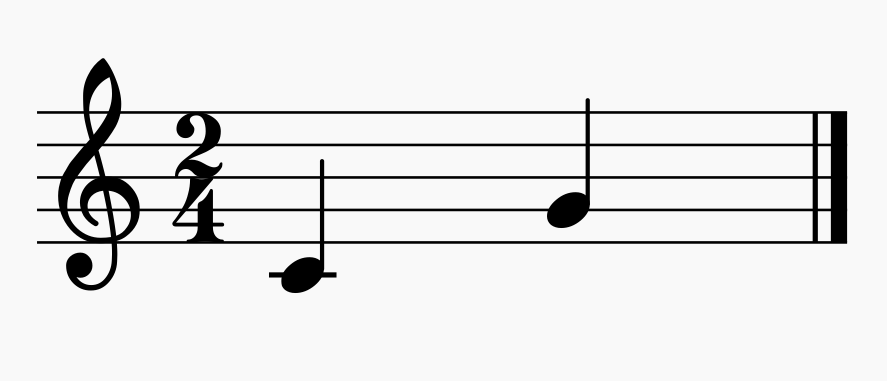
\includegraphics[width=0.4\linewidth]{imagenes/example_notes.png}
	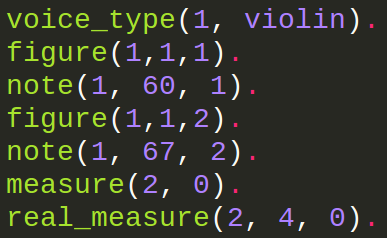
\includegraphics[width=0.4\linewidth]{imagenes/logic_facts_score.png}
	\caption{Una pieza simple transformada a hechos lógicos}
	\label{fig:simple-piece-facts}
\end{figure}

Además cuenta con parámetros en su llamada que modifican la salida producida:
\begin{itemize}
	\item \textbf{\texttt{-k}} Indica manualmente la clave en la que se armonizará la pieza en vez de detectarse automáticamente
	\item \textbf{\texttt{-s}} Especifica la cantidad de figuras consecutivas que se tienen en cuenta para la armonización
	\item \textbf{\texttt{-o}} Indica el nombre del fichero de hechos lógicos de salida	
\end{itemize}

\subsection{Núcleo ASP}
Los hechos lógicos creados por el \textit{parser} son la entrada directa del armonizador, una de las mitades del núcleo de procesado ASP de haspie.
Este módulo utiliza los hechos lógicos para expandir las reglas generales con las que cuenta, infiere nuevos predicados intermedios y asigna acordes de entre los posibles a cada tiempo de armonización especificado. Los posibles acordes se especifican en un archivo denominado \texttt{major\_chords} o \texttt{minor\_chords} según el modo en el que se esté realizando la armonización. Los acordes contemplados inicialmente por la herramienta son los acordes fundamentales de tres notas de la tonalidad, aunque se incluyó el de Dominante séptima\footnote{Acorde de cuatro notas que incorpora una nota adicional que forma un intervalo de séptima con la nota dominante de la tonalidad} para dotar al sistema de mayor naturalidad.

\begin{figure}
	\centering
	\begin{verbatim}
		1 { chord(HT,C) : pos_chord(C) } 1 :- htime(HT).
	\end{verbatim}
	\label{fig:chord-assig}
	\caption{Asignación de un único posible acorde a cada intervalo de armonización}
\end{figure}

\begin{figure}
	\centering
	\begin{verbatim}
		octave(V,((N - base) / 12),T) :- note(V,N,T), N >= 0.
		sem_tones(V,((N - base) \ 12),T) :- note(V,N,T), N >= 0.
		grade(V,1,T) :- sem_tones(V,3,T).
		grade(V,2,T) :- sem_tones(V,5,T).
		grade(V,3,T) :- sem_tones(V,7,T).
		grade(V,4,T) :- sem_tones(V,8,T).
		grade(V,5,T) :- sem_tones(V,10,T).
		grade(V,6,T) :- sem_tones(V,0,T).
		grade(V,7,T) :- sem_tones(V,2,T).
	\end{verbatim}
	\label{fig:grade-infer}
	\caption{Reglas de inferencia de Octava y Grado para una nota en el modo mayor.}
\end{figure}

Para ello, lo más importante es la conversión de los valores de las notas a grados de la escala junto con su octava, lo cual es posible conociendo la tonalidad y el modo. Con las notas transformadas en grados y todos los posibles acordes asignados, se cuantifican los errores cometidos, esto es, en vez de prohibir que se produzcan errores, se marcan aquellas notas que no pertenecen al acorde como error y se clasifican en errores fuertes y débiles atendiendo al tipo de tiempo del compás en el que coincide el error. El cálculo del tipo y subdivisión del compás, y por tanto de sus tiempos débiles y fuertes se realiza gracias a los hechos lógicos referentes al tipo de compás de la partitura y al intervalo de armonización de la misma.
Mediante un predicado de optimización que minimiza los errores en tiempos fuertes, los acordes repetidos en tiempos de armonización consecutivos y los errores cometidos en tiempos débiles (inicialmente en ese orden de importancia) se busca la mejor armonización posible.

\begin{figure}[h]
	\centering
	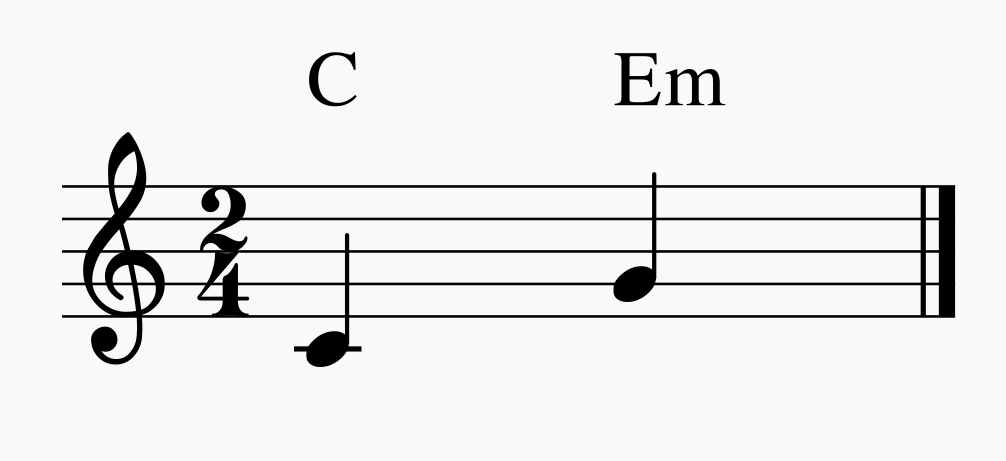
\includegraphics[width=0.4\linewidth]{imagenes/harmonized_example.png}
	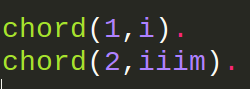
\includegraphics[width=0.4\linewidth]{imagenes/chord_facts.png}
	\caption{Acordes anotados sobre una pieza sencilla y los hechos lógicos correspondientes a esos acordes}
	\label{fig:simple-piece-chords}
\end{figure}

De vuelta al pipeline, los mejores resultados son transformados a una representación objetual en python (Ver sección \ref{subsec:store_classes}) para almacenar la información de los diferentes elementos y poder representarlos de manera sencilla. 

A continuación se pide al usuario que escoja un resultado de entre los mejores posibles, mostrándole la secuencia de acordes y especificando las notas erróneas, así como el grado de optimización del resultado. Una vez escogida la armonización deseada, se crea un fichero temporal con los acordes de la solución que se pasa, en conjunto con el fichero de hechos lógicos original al módulo de completado de partituras.

Con ambos ficheros de hechos lógicos, se llama al módulo de completado de partituras, que actuará en caso de existir voces nuevas que completar o secciones en blanco que rellenar. Los intervalos a rellenar están representados por el hecho lógico especial \texttt{freebeat} que indica que ese tiempo no contiene una nota sino un hueco intencialmente blanco. No obstante, estos hechos van acompañados de un hecho \texttt{figure} al igual que las notas o silencios, de modo que se puede especificar el patrón rítmico de la sección a completar.
El módulo de completado de partituras funciona de un modo similar al de acordes, asignando nuevas notas a los espacios en los cuales se le pida que lo haga. La principal diferencia es que no cuenta con un fichero de notas posibles como el módulo de armonización con los acordes, sino que utiliza el valor numérico de la nota directamente. 

\begin{figure}
	\centering
	\begin{verbatim}
		1 { freebeatfigure(V,N,1,FB) : N=VL..VH } 1 :- freebeat(V,FB),
		                 voice_limit_low(V,VL), voice_limit_high(V,VH).
	\end{verbatim}
	\label{fig:note-assig}
	\caption{Asignación de nuevas notas a espacios en blanco, respetando la tesitura especificada}
\end{figure}

Para limitar el espacio de búsqueda, estos valores son únicamente los comprendidos entre los límites definidos por la tesitura del instrumento de la voz que se esta está completando. De manera parecida al fichero de definición de los acordes de cada modo, se han definido las tesituras de algunas de las voces corales más frecuentes junto con algunos instrumentos como el violín o el violonchelo, así mismo este fichero puede ser fácilmente editado por el usuario para incluír nuevas tesituras o instrumentos.

\begin{figure}
	\centering
	\begin{tabular}{ | l | c | c | }
		\hline
		Tesitura & Nota mínima & Nota máxima \\ \hline \hline
		Bajo & 40 & 64 \\ \hline
		Barítono & 45 & 69 \\ \hline
		Tenor & 48 & 72 \\ \hline
		Contra-Tenor & 52 & 76 \\ \hline
		\hline
		Contralto & 53 & 77 \\ \hline
		Mezzo-Soprano & 57 & 81 \\ \hline
		Soprano & 60 & 84 \\ \hline
	\end{tabular}
	\label{fig:tesiturae}
	\caption{Relación de tesituras corales y sus límites inferior y superior}
\end{figure}

Estas nuevas notas se transforman a grados y octavas como ya se hace con las notas de entrada del módulo de armonización para poder ser cotejadas contra la armonía especificada por el módulo anterior. Del mismo modo que en el módulo de armonización se cuantifican y categorizan los errores porducidos por estas nuevas notas en relación a la armonía establecida y, minimizándolos, se buscan los mejores resultados. Gracias a los hechos lógicos \texttt{figure} de la entrada, el módulo de completado reconstruye las figuras originales.

\begin{figure}
	\centering
	\begin{verbatim}
		octave_jump(V,B1,B2) :- ex_note(V,N1,B1), ex_note(V,N2,B2),
		                     (B1+1) == B2, N2 > (N1+12), beat(B1+1).
		octave_jump(V,B1,B2) :- ex_note(V,N1,B1), ex_note(V,N2,B2),
		                     (B1+1) == B2, N2 < (N1-12), beat(B1+1).
		:- octave_jump(_,_,_).
	\end{verbatim}
	\label{fig:octave-jump}
	\caption{Definición de salto de octava para las notas generadas y restricción que lo prohibe}
\end{figure}

\begin{figure}[h]
	\centering
	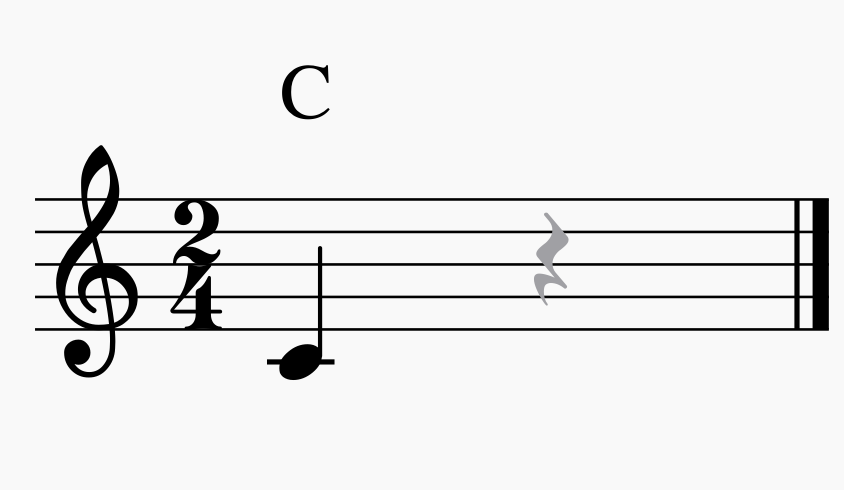
\includegraphics[width=0.4\linewidth]{imagenes/incomplete_score.png}
	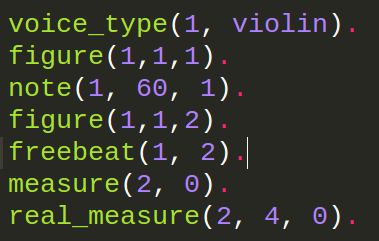
\includegraphics[width=0.4\linewidth]{imagenes/incomplete_facts.png}
	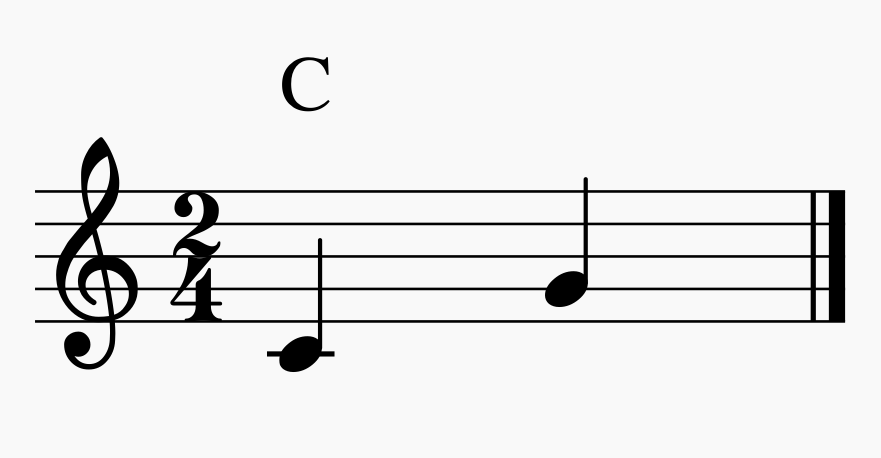
\includegraphics[width=0.6\linewidth]{imagenes/completed_score.png}
	\caption{Partitura armonizada con un tiempo incompleto y resultado del completado}
	\label{fig:simple-piece-complete}
\end{figure}

Repitiendo el proceso anterior, el pipeline procesa la salida de clasp y la almacena en las clases de almacenamiento correspondientes. Tras esto muestra las mejores soluciones de completado al usuario y permite escoger una de ellas. Al hacerlo los objetos de almacenamiento generados se pasan al módulo de salida para su representación final.

\subsection{Módulos de Preferencias}
Se han especificado, a mayores de los módulos principales ya descritos, dos submódulos adicionales que mejoran los resultados del módulo completador de partituras.

El primero es un módulo de preferncias melódicas. Sirve para compensar la ausencia de composición melódica en haspie creando partituras más cantables o melódicas. Contiene reglas que:
\begin{itemize}
	\item Definen la tendencia de una voz ya existente en la partitura y permiten al completador de partituras componer de forma que se imite dicha tendencia
	\item Miden los saltos melódicos entre las notas de una misma voz e intentan acortarlos haciendo que la progresión melódica sea más cantable.
\end{itemize}

Para la tendencia, se mide si en un intervalo determinado, el valor de notas consecutivas crece o decrece y mediante una regla que establece el tipo de tendencia (semejante u opuesta) al procesar multiples voces al mismo tiempo. Por otra parte, para los saltos melódicos se crean nuevos predicados \texttt{melodic\_jump} teniendo en cuenta la diferencia de los valores de notas consecutivas en una misma voz.

\begin{figure} [h]
	\centering
	\begin{verbatim}
		melodic_jump(V,J,B1,B2) :- out_note(V,N1,B1), out_note(V,N2,B2),
		                       (B1+1) == B2, beat(B1+1), J = #abs(N1-N2). 
	\end{verbatim}
	\label{fig:melodic-jump}
	\caption{Definición de salto melódico}
\end{figure}


El segundo módulo detecta progresiones de un determinado tipo de acordes (inversiones de cuarta y sexta). Este tipo de progresión es muy común en música coral, y por tanto, los resultados usando este módulo con piezas corales resultan mucho más realistas. Para esto se realiza una armonización a tiempo, es decir, se asigna un acorde a cada instante de la pieza y se intentan detectar estas progresiones concretas de acordes con el fin de crearlas o continuarlas si ya existen con la ayuda de las nuevas notas generadas. Es debido a esta armonización a tiempo que este módulo es tremendamente pesado computacionalmente.

\subsection{Ficheros de Configuración}
Las reglas de optimización, ya sean maximización o minimización, presentes en los módulos y submódulos ASP asignan un peso y un orden de relevancia a los predicados que se cuantifican de cara a la optimización. Este peso por defecto puede ser sobreescrito mediante ficheros de configuración. Cambiando el peso de cada hecho se altera como de importante es la aparición de cada uno de esos hechos, mientras que cambiando el orden de relavancia se determina como se realizará el proceso de optimización al completo.
Se presenta un fichero de configuración de ejemplo comentado para que el usuario pueda cambiar el funcionamiento de la herramienta a su antojo, produciendo cambios drásticos en el estilo con un esfuerzo mínimo y permitiendo almacenar estas preferencias en un fichero que determine su estilo personal de composición.

\subsection{Clases de Almacenamiento}
\label{subsec:store_classes}
Para poder almacenar temporalmente los resultados de los dos submódulos ASP de haspie se diseñaron e implementaron clases de almacenamiento que se corresponden con los diferentes hechos lógicos que los módulos ofrecen en su salida. El diagrama de clases de estos objetos de almacenamiento puede consultarse en el anexo \ref{chap:diagrams}. Se dividen en dos jerarquías, una para los resultados del módulo de armonización y otra, considerablemente más grande para el módulo de completado de partituras. 
En cuanto al módulo de armonización, éste cuenta con las siguiente clases:
\begin{itemize}
	\item \texttt{\textbf{ClaspChords:}} Almacena todas las solcuiones del armonizador, tanto en texto plano como en un array de objetos \texttt{ChordSolution}. Posee un método para transformar la salida de clasp a los diferentes objetos de la jerarquía.
	\item \texttt{\textbf{ChordSolution:}} Contiene dos listas ordenadas, una de objetos \texttt{Error} y otra de objetos \texttt{Chord}, y un valor de optimización que mide como de buena es la solución.
	\item \texttt{\textbf{Error:}} Representa una nota errónea en la partitura, especificando voz y tiempo para ubicarla en ella, así como el grado musical que produce el error.
	\item \texttt{\textbf{Chord:}} Representa un acorde en la pieza, especificando el nombre del mismo y el tiempo al que ha sido asignado.
\end{itemize}

Las clases para almacenar la información de la salida del módulo de completado de partituras siguen una estructura similar al de armonización, pero la jerarquía es algo más compleja al tener mucha más información que representar:
\begin{itemize}
	\item \texttt{\textbf{ClaspResult:}} Funciona de modo muy similar a \texttt{ClaspChords}. Almacena todas las solcuiones del completador de partituras, tanto en texto plano como en un array de objetos \texttt{HaspSolution}. Posee un método para transformar la salida de clasp a los diferentes objetos de la jerarquía. 
	\item \texttt{\textbf{HaspSolution:}} De forma parecida a \texttt{ChordSolution}, almacena los diferentes objetos de la solución. La principal diferencia radica en que hace uso de un diccionario de datos, siendo los índices cada una de las voces de la pieza y almacenando en la entrada de cada índice una lista ordenada de los diferentes objetos de la partitura.
	\item \texttt{\textbf{Error:}} Funciona igual que \texttt{Error} en la jerarquía de clases del módulo de armonización. Representa una nota errónea en la partitura, especificando voz y tiempo para ubicarla en ella, así como el grado musical que produce el error.
	\item \texttt{\textbf{PassingNote:}} Nota errónea que cumple unas características particulares, como su ubicación en un tiempo débil de la partitura. Especifica la voz y el tiempo en el que se produce, de modo similar a \texttt{Error}.
	\item \texttt{\textbf{Chord:}} Similar a \texttt{Chord} en la jerarquía de clases del módulo de armonización. Representa un acorde en la pieza, especificando el nombre del mismo y el tiempo al que ha sido asignado.
	\item \texttt{\textbf{VoiceType:}} Indica el nombre asignado a una voz, es decir, el instrumento que la interpreta.
	\item \texttt{\textbf{Note:}} Especifica la voz y tiempo en los que suena la nota, así como su valor numérico y duración.
	\item \texttt{\textbf{Rest:}} Especifica la voz y tiempo en los que se produce el silencio así como su duración.
	\item \texttt{\textbf{Measure:}} Indica la métrica del y cantidad de notas del tipo de compás así como el tiempo en el que aparece. Se interpreta que el cambio de tipo de compás se produce en todas las voces a la vez.
	\item \texttt{\textbf{VoiceChord:}} Representa un conjunto de notas que suenan en un mismo tiempo de una sola voz, produciendo un acorde (Por ejemplo en instrumentos polifónicos como el piano o la guitarra). Contiene un array de objetos \texttt{Note} ordenados por su valor numérico, así como la voz y el tiempo en el que se produce junto con su duración.
\end{itemize}


\subsection{Salida}
El último módulo al que llama al pipeline. Haciendo uso de los objetos de representación interna, el módulo de salida genera un fichero en el formato deseado por el usuario. 
Para la implementación de este módulo se ha hecho uso de la librería Music21\footnote{http://web.mit.edu/music21/} desarrollada por miembros del MIT. Se traduce la representación interna de la partitura que el pipeline pasa al módulo de salida a la representación propia de Music21 para después con una simple llamada, reproducir o almacenar el resultado.
En este proceso de conversión, no solo se traducen las notas, voces y anotaciones de compás al formato propio de Music21, sino que además se combinan algunos de ellos para enriquecer la salida.
\begin{itemize}
	\item Los acordes, especificados en forma de grado de la tonalidad, se traducen al nombre y tipo de acorde correspondiente para ser anotados en la partitura
	\item Los errores en tiempos fuertes se marcan en la partitura coloreando en rojo las notas que los contienen
	\item Los errores en tiempos débiles se marcan en azul en la partitura indicando que son notas de paso o adornos
\end{itemize}

\begin{figure}[h]
	\centering
	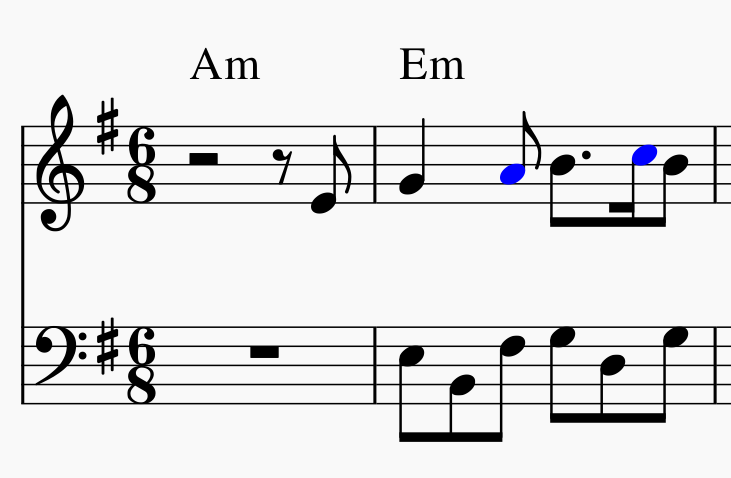
\includegraphics[width=0.6\linewidth]{imagenes/example_final_score.png}
	\caption{Partitura de ejemplo armonizada y con notas de paso coloreadas en azul}
	\label{fig:simple-piece-final}
\end{figure}


\section{Iteraciones}
Se detalla un breve resumen de cada una de las iteraciones de desarrollo del proyecto, indicando cuales fueron los progresos, cambios y refactorizaciones en cada una de ellas.

\subsection{Iteración 1}
\label{subsec:first_iteration}
Se analizaron y escogieron las diferentes tecnologías que se usarían en cada uno de los módulos de la herramienta. 
Como software de entrada para las partituras se escogió MuseScore 2, principalmente por ser \textit{opensource} y por su sencillez. Para el formato de entrada y salida, se compararon las propiedades de MIDI, LilyPond y MusicXML. Los tres formatos ofrecen posibilidades de edición, aunque cada uno sirve a un propósito diferente. MusicXML se presentó como el formato idóneo para la tarea, ya que al ser una extensión de XML, está orientado a que una máquina pueda procesarlo y crear una estructura en memoria con toda la información que necesita para poder extraer los datos de la partitura. Además, la implementación del \textit{parser} para un lenguaje etiquetado como XML es un problema convencional y relativamente sencillo.

Para el procesador de XML a hechos ASP se optó por las bibliotecas Flex y Bison para C. EL principal motivo para ello fue que fueron las tecnologías empleadas en la asignatura Procesamiento de Lenguajes y durante una de las prácticas de la misma se desarrolló una primera versión de este mismo procesador que ahora se usa en el proyecto. Además Flex y Bison garantizan velocidad y eficiencia en el procesado. Por último pero no menos importante, y ya que el proyecto se está enfocando desde un punto de vista de desarrollo ágil, actualizar los ficheros de código de Flex y Bison es realmente sencillo, lo cual permitiría añadir nuevos elementos a reconocer cuando sea necesario.

Se procedió a desarrollar una versión actualizada de dicho parser. Las pruebas realizadas al \textit{parser} revelaron que existía un problema de análisis al no poder verificar de forma sencilla que cada etiqueta se cerraba de modo correcto, es decir, que el nombre de la etiqueta que cierra un bloque sea el mismo del que la abrió, se implementó una pila en C para esta tarea. 

\begin{figure}
	\centering
	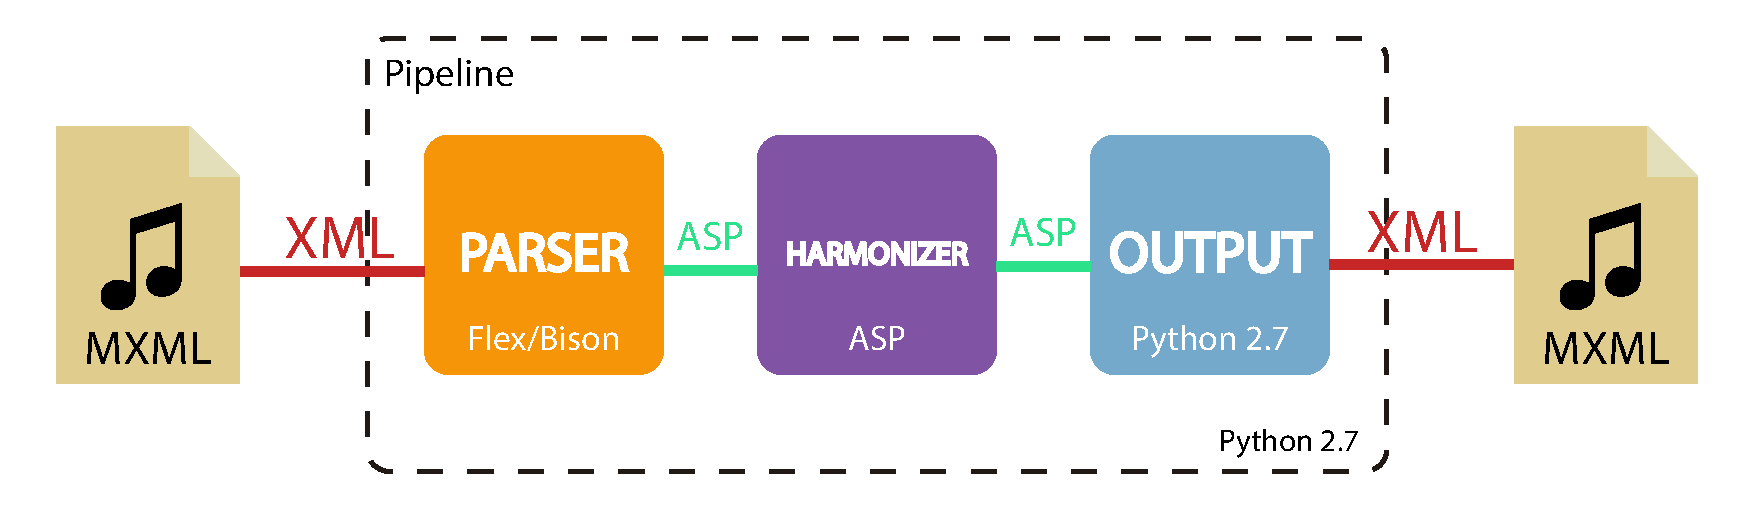
\includegraphics[width=0.8\linewidth]{imagenes/arquitectura_inicial.pdf}
	\caption{Diagrama del planteamiento inicial de la arquitectura del sistema}
	\label{fig:arquitectura_inicial}
\end{figure}

\subsection{Iteración 2}
\label{sec:second_iteration}
Se modificó el procesador de MXML a ASP y se incluyó una opción para subdividir la partitura de forma automática en base a la nota más breve de la partitura o forzar toda la partitura a un solo tipo de figura omitiendo aquellas figuras de menor duración.

En esta primera aproximación, se crearon las primeras reglas del módulo de armonización, que realizan una asignación acorde-unidad rítmica en base a las notas presentes para un instante dado en cada voz. Se crearon dos ficheros a mayores que especifican los acordes a considerar por la herramienta, según si la armonización se realiza en modo mayor o menor. 

A mayores se incluyó como parte de esta iteración, el diseño e implementación de un pipeline en python que automatiza las llamadas al procesador MXML a hechos ASP y al módulo de armonización. En este primer prototipo se implementó una pequeña funcionalidad de interpretación de la salida del módulo ASP a un vector de soluciones.


\subsection{Iteración 3}
\label{subsec:third_iteration}
Se modificó el \textit{parser} substancialmente ya que este imprimía a un fichero según procesaba las notas. Esto no planteaba problema alguno si la subdivisión se especificaba de antemano mediante el parámetro correspondiente, pero sí que resultaba complicado mantener esta aproximación si la unidad de subdivisión debía calcularse al mismo tiempo que se procesaba la partitura en MusicXML. Se plantearon dos soluciones: o bien incluir en el pipeline en python un análisis previo a la conversión de MXML a hechos en ASP que dedujese cual era la nota de menor longitud y la usase como parámetro en la llamada al \textit{parser} o bien se modificaba el comportamiento del anterior para realizar simultáneamente ambas tareas. 

Se optó por la segunda opción por motivos de coherencia con el sistema, es decir, no incluir funcionalidad innecesaria y replicada en el pipeline, cuya tarea es simplemente manejar las entradas y salidas de los diferentes módulos, y por motivos de eficiencia, ya que como se ha mencionado no hay necesidad de procesar el mismo fichero dos veces, siendo una de ellas en un lenguaje interpretado en vez de compilado, lo que añadiría un sobrecoste temporal evitable.

Los cambios implementados en el \textit{parser} conllevaron incluir un nuevo tipo de dato nota para almacenar la información de las notas de la partitura y una nueva pila que contuviese las notas extraídas del MXML.

En el módulo de armonización se incluyó una nueva constante que indica la longitud del intervalo de tiempo mínimo de análisis armónico horizontal. Se modificaron, por tanto, las reglas de asignación de acordes para poder usar el intervalo especificado. Además se suavizaron las restricciones que podaban las soluciones erróneas y en vez de ello, generan un nuevo predicado error(voz, grado, tiempo) que indica los grados erróneos presentes en la partitura que no encajan con el acorde asignado para la solución. 

 Se han implementado en el pipeline, con vistas al futuro de módulo de salida, una serie de clases para procesar y almacenar los resultados de clasp y poder devolverlos más tarde en el formato más conveniente. Concretamente, en esta iteración se implementaron las primeras versiones de \texttt{Error}, \texttt{Chord}, \texttt{HaspSolution} y \texttt{ClaspResult}.

\subsection{Iteración 4}
\label{sec:fourth_iteration}
El módulo ASP se ha aumentado para incluir generación de notas en un número de voces adicionales que puede ser especificado por parámetro. Además se refactorizaron algunas reglas y se creó un fichero de conversiones encargado de traducir valores de notas a grados, octavas y viceversa. Para la generación de notas en las nuevas voces se ha impuesto una única restricción fuerte: que dos notas consecutivas no realicen un salto melódico de más de una octava.

Se optó por incorporar \textbf{Music21} al módulo de salida. Principalmente por la cantidad de formatos con los que puede trabajar, tanto en entrada como en salida, y aunque lo ideal será exportar un fichero MusicXML, la idea de poder generar PDF, MIDI o Lilypond resulta más que atractiva. Este módulo toma un objeto \texttt{HaspSolution} y, previa transformación a la representación interna de Music21, lo representa en el formato adecuado para ser reproducido o almacenado.  

En el \textit{pipeline} se ha incluyó la opción de especificar el número de voces adicionales que deben ser añadidas y otra opción para especificar el formato de salida. A mayores, se incluyó una llamada al módulo de salida en el pipeline.

\subsection{Iteración 5}
\label{subsec:fifth_iteration}
En el procesador de MusicXML a hechos lógicos ASP se han incluido dos nuevas funciones principales: 
\begin{itemize}
	\item \textbf{Análisis de medida de compás:} Determinar cuantas figuras de qué longitud posee el tipo de compás base de la pieza.
	\item \textbf{Distincisón de tipos de silencios:} Diferenciar silencios completables de aquellos que deben ser respetados como silencios.
\end{itemize}

Para la métrica del compás, se implementó en el procesador la capacidad de identificar los diferentes tipos de compases así como el tiempo en el que ocurren, aunque por comodidad y sencillez, se ha asumido que un cambio rítmico en el compás debe ocurrir en todas las voces a la vez. El tipo de compás además es modificado según la nota mñas breve de la partitura para que no existan problemas a la hora de comparar la cantidad y el tipo de figuras del compás.

Para poder especificar en el editor de partituras silencios ``verdaderos'' y silencios completables se optó por una solución relativamente sencilla, no sólo de identificar por el \textit{parser} si no también fácil de usar por el usuario final de la herramienta. Mediante la notación de letras de la pieza, se pueden indicar en cada voz los intervalos de tiempo en los cuales los silencios deben ser tratados como completables. Para ello solo hace falta escribir los símbolos \texttt{[} y \texttt{]} al principio y final del intervalo respectivamente. Para poder detectar este intervalo se incorporó un tipo de dato cola genérica al procesador para poder interpretar bien el momento de inicio y de cierre de estos símbolos y marcar así los intervalos a completar de manera adecuada.

En el módulo de armonización se han definido acordemente varios predicados nuevos, que representan los tiempos completables de cada voz. A mayores de crearon reglas para identificar la subdivisión de los compases con el fin de inferir los tiempos fuertes y débiles de cada compás en la partitura. Gracias a esto se han creado predicados que matizan los diferentes errores de la partitura según el tipo de tiempo en el que ocurren los errores de la pieza y permite minimizarlos con diferentes prioridad (a más fortaleza de tiempo, más prioridad). Por último y para dar más flexibilidad en la búsqueda de la armonización correcta se ha incluído el acorde de dominante séptima (V7) en los modos mayor y menor.

Se ha incluido una clase de almacenamiento \texttt{Rest} para diferenciarla de \texttt{Note}. Ya que las entradas del diccionario que representa las diferentes voces de la partitura puede almacenar cualquier combinación de tipos de elementos, se estableció una convención para poder almacenarlos e iterar sobre ellos sin problema.

El módulo de salida se ha refinado para representar mejor las notas incluyendo información del tipo de compás, clave y duración de las figuras. Además se colorean en rojo los errores detectados y se anotan en los tiempos adecuados los acordes inferidos por el módulo ASP.

Por último, el pipeline cuenta con una nueva opción que permite especificar un tiempo máximo de búsqueda del óptimo en el módulo ASP, ya que para piezas largas, el espacio de búsqueda crece muchísimo y es necesario poder limitar el tiempo de ejecución.

\subsection{Iteración 6}
\label{sec:sixth_iteration}

Para facilitar la entrada de silencios que representan huecos completables por el módulo ASP se cambió el enfoque, y se abandonó el delimitado de secciones completables con corchetes en las letras de la canción por suponer algunos problemas al no poder ubicar dichas letras en tiempos en los que haya un silencio, por claridad y por no interferir con las posibles letras de una partitura real no creada ni modificada \textit{ad-hoc} para el programa. MusicXML permite marcar elementos de la partitura como no visibles, esto solo afecta a la hora de imprimir en papel dicha partitura y a nivel musical no interfiere con ningún elemento. Además, la visibilidad de una nota o silencio puede ser fácilmente alterada en cualquier editor de partituras desmarcando una casilla al clicar sobre dicho elemento, lo cual facilita mucho el marcado de estos tiempos completables. Esto se reflejó en el procesador de MusicXML a hechos lógicos, que en vez de contemplar los dos símbolos utilizados anteriormente, ahora solo tiene que comprobar la visibilidad de un elemento para determinar si asignar un tiempo completable a dicho tiempo.

Para refinar la subdivisión en tiempos débiles y fuertes, se reimplementaron tanto en el módulo ASP como en el procesador de hechos lógicos a MusicXML, esto fue debido a que no es sencillo establecer dichos tiempos aritméticamente sólo teniendo en cuenta la cantidad de notas del compás, sino que también se ha de tener en cuenta el tipo y subdivisión del compás con respecto a la nota de referencia usada para armonizar. Para esto es importante no normalizar el compás leído en el fichero XML y generar nuevos predicados indicando los valores del compás sin modificar. En el módulo ASP se ha incluido, de modo similar a los acordes, una tabla de tipos de compás y su subdivisión teniendo en cuenta el compás y la longitud del tiempo de armonización. Se han incluido en dicha tabla los compases más habituales. 

Se creó el sub-módulo ASP de preferencias melódicas que busca alcanzar una optimización mayor a la hora de generar nuevas voces o cubrir tiempos completables con algunas mejoras que atienden, principalmente, a la secuencia de notas de una misma voz. Se incluyó también en este sub-módulo de preferencias melódicas la detección de patrones de secuencias de sextas.

Se ha descartado la detección de apoyaturas con el fin de no contemplarlas como errores por un motivo similar, al uniformizar la longitud de las figuras de la partitura, no es posible detectarlas bien, ya que una de las características de las apoyaturas es que ``roban'' brevemente el tiempo fuerte a una nota representativa del acorde de la armonía.

\subsection{Iteración 7}
\label{subsec:seventh_iteration}

Se incluyeron en el \textit{parser} nuevos \textit{tokens} y reglas en la gramática para poder extraer metadatos y otra información de la partitura y exportarlos a un fichero temporal usado por el módulo de salida. Los diferentes datos extraídos para cada partitura son:
\begin{itemize}
	\item \textbf{title:} Título
	\item \textbf{composer:} Compositor
	\item \textbf{base\_note:} Longitud de la nota más breve presente
	\item \textbf{key\_name:} Nombre de la clave en la que se armonizará la pieza
	\item \textbf{mode:} Modo (mayor o menor)
	\item \textbf{last\_voice:} Número que identifica cual es la última voz presente
\end{itemize}

El procesador extrae una nueva pieza de información de la partitura, conocida como \texttt{figure}. Figure es un hecho lógico que describe la duración de una figura para un pulso de una voz dada. De este modo, pese a subdividir las notas a la longitud de la más breve para el análisis, se pueden recomponer en la salida fidedignamente. Se han incluido reglas adicionales para reconocer los acordes presentes en la partitura y estos se plasman en el fichero de salida.

En el módulo de armonización se ha incluido un nuevo archivo similar al de acordes o tipos de compases que describe las diferentes tesituras de las voces presentes en la partitura. Este documento es ampliable al igual que los mencionados para incluir nuevos instrumentos o tesituras. Se han definido los principales tipos de voz coral (tanto masculinos como femeninos) y sus rangos de notas más frecuentes. 

Además el módulo de armonización se añadieron reglas para tener en cuenta los nuevos hechos \texttt{figure} y utilizarlos para generar los patrones rítmicos adecuados en las secciones a completar. Para este mismo módulo se corrigió el archivo de preferencias de enlace de sextas, ahora separado del archivo de preferencias melódicas. Por último se ha adaptado la salida para trabjar con un nuevo hecho lógico que conjuga las notas con las figuras para producir un unico hechoconjunto con toda la información necesaria.

Se ha definido una nueva clase \texttt{VoiceChord}, que representa un acorde realizado por un solo instrumento polifónico ya que los este tipo de acordes producían fallos en la anterior iteración. Para su correcto funcionamiento se modificó la pequeña rutina de transformación de hechos lógicos de la salida del módulo de armonización para tener en cuenta la posibilidad de que existiesen varias notas en un mismo pulso de una voz y agregarlas en un objeto VoiceChord.

En el módulo de salida se han corregido algunos errores encontrados en las iteraciones anteriores y haciendo uso de los nuevos hechos lógicos de la iteración, se puede reconstruir la partitura mucho mejor que antes. Además el módulo de salida tiene en cuenta y representa correctamente el nuevo elemento \texttt{VoiceChord} y en la partitura además se escribe en la clave especificada o detectada por el procesador. Por último, se ha incluido una nueva funcionalidad para leer del archivo de temporal de configuracion de la partitura los metadatos de título y compositor, junto con los nombres de los instrumentos de cada pentagrama, que son asignados a cada una de las voces de la partitura de salida.

Los nuevos datos extraídos por el procesador son leídos desde el pipeline y son pasados a los subsiguientes módulos de armonización y salida respectivamente. Se ha modificado el parámetro -v del pipeline y su efecto en el resto de módulos. En vez de especificar una cantidad de voces a añadir, toma como mínimo un argumento indicando la tesitura (por nombre) o el rango de notas para las nuevas voces. El pipeline se encarga de crear, a partir de los datos de este parámetro -v un nuevo fichero temporal \texttt{extra\_voices.lp} que será incluido en la llamada del módulo de armonización para que dichas nuevas voces se tengan en cuenta. Se incluyó una opción que permite especificar manualmente la clave de la partitura mediante la letra de nota base de la escala en la que se quiere armonizar la pieza. De no ser especificada esta se calcula automáticamente. Cuenta además con otra opción que permite incluir la preferencia de los enlaces de sextas.

Tras probar el prototipo de esta iteración se llegó a la conclusión de que había dos factores ralentizando el proceso:
\begin{itemize}
	\item La armonización se realizaba junto con el completado de voces y espacios en blanco, con lo cual ASP debía generar todas las posibles combinaciones de notas para todas las posibles armonizaciones.
	\item La generación de notas se calculaba para cualquier rango y después se restringía para la tesitura correcta en vez de generar notas entre los límites de la tesitura. 
\end{itemize}

\subsection{Iteración 8}
\label{subsec:eighth_iteration}
Se tomó la decisión de dividir el módulo de armonización en dos sub-módulos ASP:
\begin{itemize}
	\item \textbf{Armonización:} Busca fijar una armonización ofreciendo al usuario diferentes soluciones ordenadas según unos valores de optimización.
	\item \textbf{Completado:} Su trabajo será, una vez establecida la armonización deseada, completar la partitura de modo similar a como se realizaba antes.
\end{itemize}

Se realizaron cambios menores en ambas partes para adecuarlas a sus nuevas tareas, se eliminaron muchos componentes de salida y ciertas reglas de generación de predicados ahora inútiles en la asignación de acordes y se revisó el módulo de generación de notas para eliminar todo aquello referente a la asignación de acordes. Además en el módulo de generación de notas se restringió la generación de las mismas a aquellas posibles dentro de la tesitura de la voz.

Se diferenciaron los hechos \texttt{freebeat}, generados por el procesador y por tanto con un \texttt{figure} relacionado, de los pulsos a rellenar de las voces nuevas. Estos \texttt{newvoicebeat} se utilizan para realizar la asignación de las nuevas figuras y notas, de modo que ya se cree la figura de salida desde el principio. 
	
Para posibilitar la configuración de pesos y orden de optimización en los diferentes módulos y archivos de preferencias se cambiaron los valores constantes de las reglas de optimización por nombres de valores especificados en cada uno de los ficheros para que sirvan de valores por defecto. Se investigó sobre el orden de precedencia de los valores asignados a constantes en ASP y se descubrió que no se puede redefinir valores constantes y que el primer valor que toma es el usado. Esto se aplica a ficheros de configuración y los parámetros pasados por línea de comandos. Teniendo esto en mente, se creó un fichero de configuración \texttt{sample.lp} en la nueva carpeta pref, destinada a almacenar los diferentes ficheros de configuración de preferencias. Si este fichero se incluye en la llamada a clingo antes que cualquier otro fichero, los valores definidos en él serán los que se usen en el proceso de armonización y completado. Si alguno de los valores se borra en este fichero, se usará el valor por defecto. Además para poder trabajar con los módulos de preferencias opcionales que también contienen pesos y orden de optimización, se modificó el orden en el que estos ficheros se incluyen en la llamada a clingo.

Debido a estos cambios se modificaron las clases de almacenamiento para reflejar los resultados de la armonización y el completado de forma separada. De modo paralelo a las clases de almacenamiento \texttt{ClaspResult} y \texttt{HaspSolution} se crearon \texttt{ClaspChords} y \texttt{ChordSolution}.

Se revisaron errores producidos en la interpretación de los valores de las notas alteradas. El error se debía a una mala identificación por parte del \textit{parser} de los valores que podía tomar la etiqueta \texttt{alteration}. Se revisó también este módulo para corregir otro error que afectaba a instrumentos de varios pentagramas, donde las diferentes partes se dvididían en diferentes voces pero no se asignaba el nombre del instrumento de forma correcta a otras voces que no fuesen la primera.

Durante las pruebas finales se detectó un tipo de silencio no reconocido correctamente, este silencio usaba el símbolo de un silencio de blanca pero ocupaba todo el compás siempre, fuese cual fuese su duración. Tal y como estaba diseñado el procesador, que identificaba el tipo de figura y la subdividía cuando fuese necesario, este tipo de figuras eran irreconocibles y se tuvo que implementar un caso especifico para estos silencios especiales. 

En el pipeline se incluyeron dos nuevas opciones. Una para establecer el número máximo de soluciones deseadas y otra que permite pasarle a los módulos de armonización y completado de partitura el fichero de configuración deseado. Se cambió ligeramente el comportamiento del pipeline al tener que realizar las llamadas a los dos nuevos sub-módulos ASP, parando tras hallar las mejores armonizaciones y ofreciendo al usuario seleccionar la deseada y pasando el resultado al sub-módulo de completado, donde la ejecución continúa de modo similar a los anteriores prototipos. Por último se modificó la opción que permite especificar el tiempo límite de búsqueda para ser solo usada en caso de querer buscar todos los óptimos en vez de quedarse con el primero encontrado.



 \chapter{Evaluation}
\label{chap:evaluation}
\vspace{0.5cm}

%%%%%%%%%%%%%%%%%%%%%%%%%%%%%%%%%%%%%%%%%%%%%%%%%%%%%%%%%%%%%%%%%%%%%%%%%%%%%%%%
% Objetivo: Exponer los resultados objetivos del sistema                       %
%%%%%%%%%%%%%%%%%%%%%%%%%%%%%%%%%%%%%%%%%%%%%%%%%%%%%%%%%%%%%%%%%%%%%%%%%%%%%%%%

 \lettrine{E}{n} este capítulo exponen los resultados de la evaluación del sistema. Se han seleccionado tres piezas musicales conocidas para realizar las diferentes pruebas. A continuación se describen las tres piezas y las pruebas realizadas. Para realizar una prueba de carga que establezca los límites del sistema se ha añadido una última partitura suficientemente sencilla sobre la que trabajar para poder realizar estas pruebas cómodamente sin preocuparse por la calidad de los resultados.
 
 \lettrine{F}or the tool's evaluation, three pieces were chosen to test the different aspects of the tool. To perform a workload test of the tool, a last simple piece was added to these three first pieces, just to measure execution times, regardless of the quality of the results.
 
 \begin{itemize}
 	\item \textbf{Minuet in Major G:} Famous Johann Sebastian Bach musical piece. Interesting to check the tool's performance in ternary measures.
 	\item \textbf{Greensleves:} By Henry the VIII, it's a complex four-part polyphony, useful to check the tool's harmonization performance.
 	\item \textbf{Joy to the World:} Well known Georg F. Händel jingle.
    \item \textbf{Twinkle Twinkle Little Star:} Very simple piece to test workload and measure run times of heavy computation tasks.
 \end{itemize}
 
Using each of these pieces, the tool was asked to harmonize and complete a measure of each as well as a whole new part, measuring not only runtime but also quality of the result. Due to the non-deterministic nature of ASP, as well as the I/O times, the time measures are just to provide an approximate idea of the run times of the tool. Each measure was taken 100 times, subtracted user input time to each and then averaged.
 
\begin{figure}
	\centering
	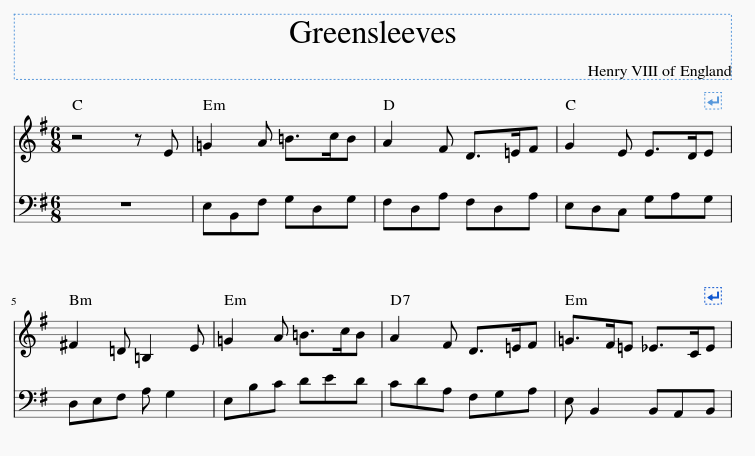
\includegraphics[width=0.8\linewidth]{imagenes/evaluation/greensleeves_harm.png}
	\caption{Harmonization result of the first measures of Greensleeves}
	\label{fig:greensleeves_harm}
\end{figure}

\begin{figure}
   	\centering
   	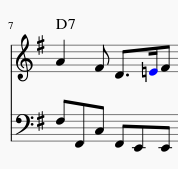
\includegraphics[width=0.2\linewidth,valign=c]{imagenes/evaluation/greensleeves_measure.png}
   	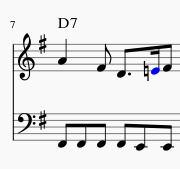
\includegraphics[width=0.2\linewidth,valign=c]{imagenes/evaluation/greensleeves_measure_melodious.png}
   	\caption{Completed single measure of Greensleves with and without melodic preferences}
   	\label{fig:greensleeves_measure}
\end{figure}

\begin{center}
	\begin{tabular}{ | l | c | c | c | }
		\hline
		Piece 			& Harmonization 	& Measure & New Part \\ \hline \hline
		Greensleeves 	& 1.016s 			& 1.926s	& 4m 49.032s \\ \hline
		Menuet 			& 0.631s 			& 0.726s 	& 3m 50.376s \\ \hline
		Joy to the World& 2.381s 			& 3.813s	& 7m 17.115s \\ \hline
		Twinkle Twinkle & 0.685s 			& 0.716s 	& 2m 31.299s \\ \hline
	\end{tabular}
\end{center}

The run time results of the tool are the expected for an ASP tool. Harmony selection times are very good and the completion times are very promising. Nevertheless, the required time to complete new parts grows very quickly as adding more and more sections to complete makes the possibilities grow exponentially.

In quality terms, the selected chords are correct, and the section completion or the new parts creation offer interesting harmonically correct solutions.

The load tests for  ``Twinkle Twinkle Little Star'' were performed by emptying progressively more and more measures of one of the parts. The piece has 24 measures, and were emptied in blocks of four. Finally more and more voices were added to the piece, achieving the following run times.
\begin{center}
	\begin{tabular}{ | l | r | }
		\hline
		Test & Time \\ \hline
		4 compases  & 1.481s \\ \hline
		8 compases 	& 2.394s \\ \hline
		12 compases	& 3.978s \\ \hline
		16 compases & 3.982s \\ \hline
		20 compases & 5.966s \\ \hline
		1 voz & 2m 31.299s \\ \hline
		2 voces & 25m 17.298s  \\ \hline
	\end{tabular}
\end{center}

\section{Comparison}
Haspie is quite unique in what it does and how does it achieve it. The only comparable tool would be ANTON \cite{anton-composing} as both use ASP to perform musical harmonization and composition and both can work over new or previously created scores.

ANTON is a way more complex system, allowing not only harmonic but melodic composition and also features rhythmic patterning, thing that haspie lacks.

Haspie is a bit more deep in harmony terms, allowing any style of musical piece to be processed, when ANTON only works with pieces of one or two voices of a certain musical style.

The tests ran for ANTON for pieces of two parts and 32 measures have run times in the minutes order, while haspie achieves a similar performance when creating a second part but it's still hard to compare, as haspie does not work in the complexity level that ANTON does.

  \section{Known Issues}
  \label{sec:known_issues}
  The tests performed revealed a few recurrent problems. In the Future Work section \ref{sec:future_work} it's detailed which of them will be addressed in short or mid term.
  
  \begin{itemize}
  		\item \textbf{Triplets:} Triplets and similar irregular figures don't work properly and need to be edited in the input score before processing it. This is because of the rhythmic standardization that the parser performs, being unable to assign correctly the time of these kind of figures.
  		\item \textbf{Key:} Some of the inferred keys are mis-interpreted in the output. This is a visual mistake more than a functional one and produces no further problems.
  		\item \textbf{Voice Names:} The locale of the system affects the parsing of the voices' names, producing some mis-interpretations.
  		\item \textbf{Falsos positivos:} Due to the simple implementation of the identification of strong and weak beats, some notes marked as mistakes or passing notes in the score may not be so.
  \end{itemize}
  
  \section{Future Work}
  \label{sec:future_work}
  The main guideline of Future Work is about developing a user friendly UI and correcting visual output errors as well as expanding the project to achieve one of the restrictions initially imposed to it, such as modulation.
 
  \subsection{Aesthetic and GUI}
  \label{subsec:look_interface}
	With the release of improved versions of the music21 library, the visual errors of the score output should be fixed. Regardless of this, there is the intention of implementing the tool as a Musescore2 plugin so the user could be able to harmonize and complete scores live, instead of having to switch back and forth between the score editor and the command line. 
  
  \subsection{Parsing and Harmonization}
  \label{subsec:parsing_harm}
  The key detection should be improved, as well as the parts name and their voice types. The strong and weak beat detection needs further work, to make it able to detect these kind of beats in complex rhythmical patterns, thus improving the harmony selection and completion results. This point also includes complex figures such as the mentioned triplets.
  
  \subsection{Modulation}
  \label{subsec:future_modulation}
  Modulation was one of the self imposed restrictions of the project to keep it's development time in check. Not only is hard to parse and detect but also presents problems to the tool due to it's way of detecting the best chords and the way it completes blank sections. The main approach for this should be splitting the score in sub-scores, preforming the current steps and finally re-assembling it.
  
  \subsection{Publishing}
  \label{subsec:releasing}
  After making the tool more user friendly and fixing some of the tool's limitation, professionals of the music teaching sector should be contacted to provide feedback and to further improve the tool so it can finally fulfill it's role as a full-fledged music learning tool.



 %%%%%%%%%%%%%%%%%%%%%%%%%%%%%%%%%%%%%%%%
 % Apéndices, glosarios y bibliografía  %
 %%%%%%%%%%%%%%%%%%%%%%%%%%%%%%%%%%%%%%%%
 \appendix
 \newpage
\chapter{Diagramas}
\label{chap:diagrams}
La herramienta no hace un uso intensivo de la orientación a objetos, en lo referente a herencia, composición, clases abstractas y similares. No obstante sí que existe una jerarquía de objetos de almacenamiento y representación de los hechos lógicos representados a la salida de los diferentes módulos. Con respecto al diagrama de secuencia, su ausencia es justificable ya que no ilustra nada ni sirve a ningún propósito real. El diagrama de arquitectura aclara mucho mejor el funcionamiento y el flujo de datos entre los módulos del sistema que cualquier diagrama de secuencia, ya que los diferentes módulos se invocan secuencialmente y la salida de cada uno se recibe en el pipeline y se pasa al siguiente módulo hasta terminar.

\begin{figure}[th]
	\centering
	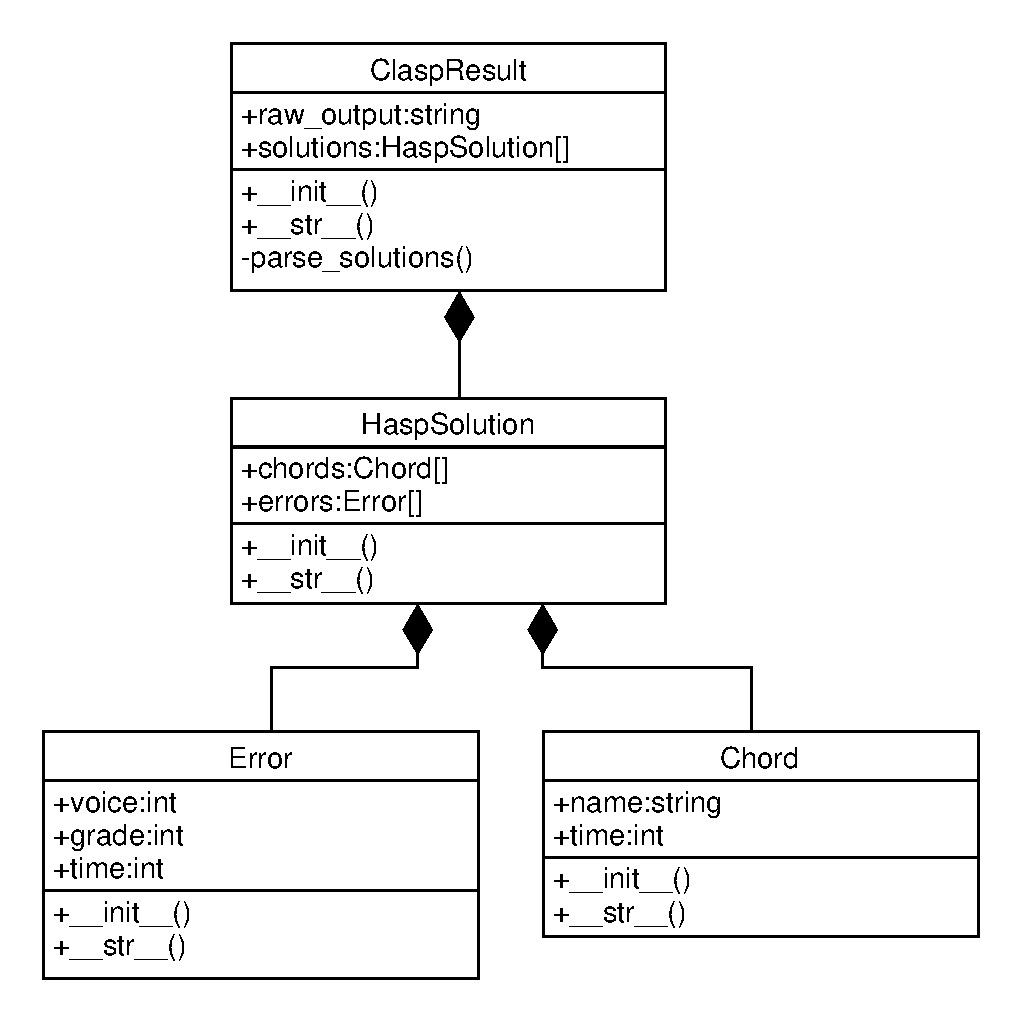
\includegraphics[width=0.8\linewidth]{imagenes/third_iter.pdf}
	\caption{Diagrama de clases de almacenamiento de la Iteración 3}
	\label{fig:class_diagram_third}
\end{figure}
\newpage
\begin{figure}[th]
	\centering
	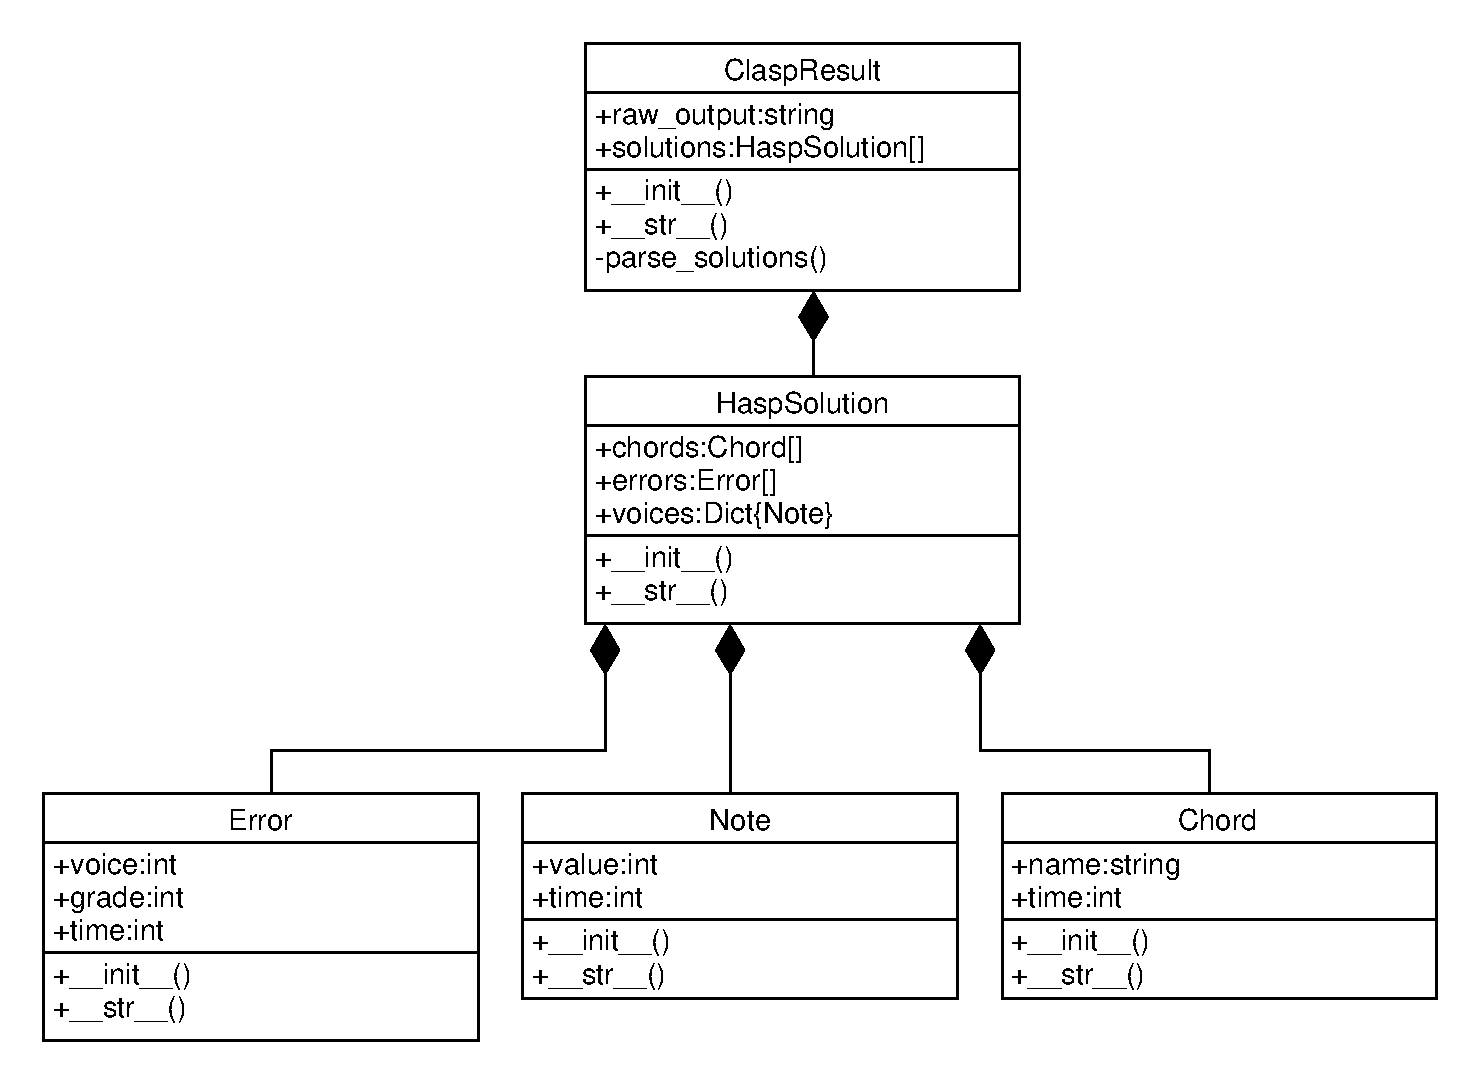
\includegraphics[width=0.8\linewidth]{imagenes/fourth_iter.pdf}
	\caption{Diagrama de clases de almacenamiento de la Iteración 4}
	\label{fig:class_diagram_fourth}
\end{figure}
\begin{figure}[th]
	\centering
	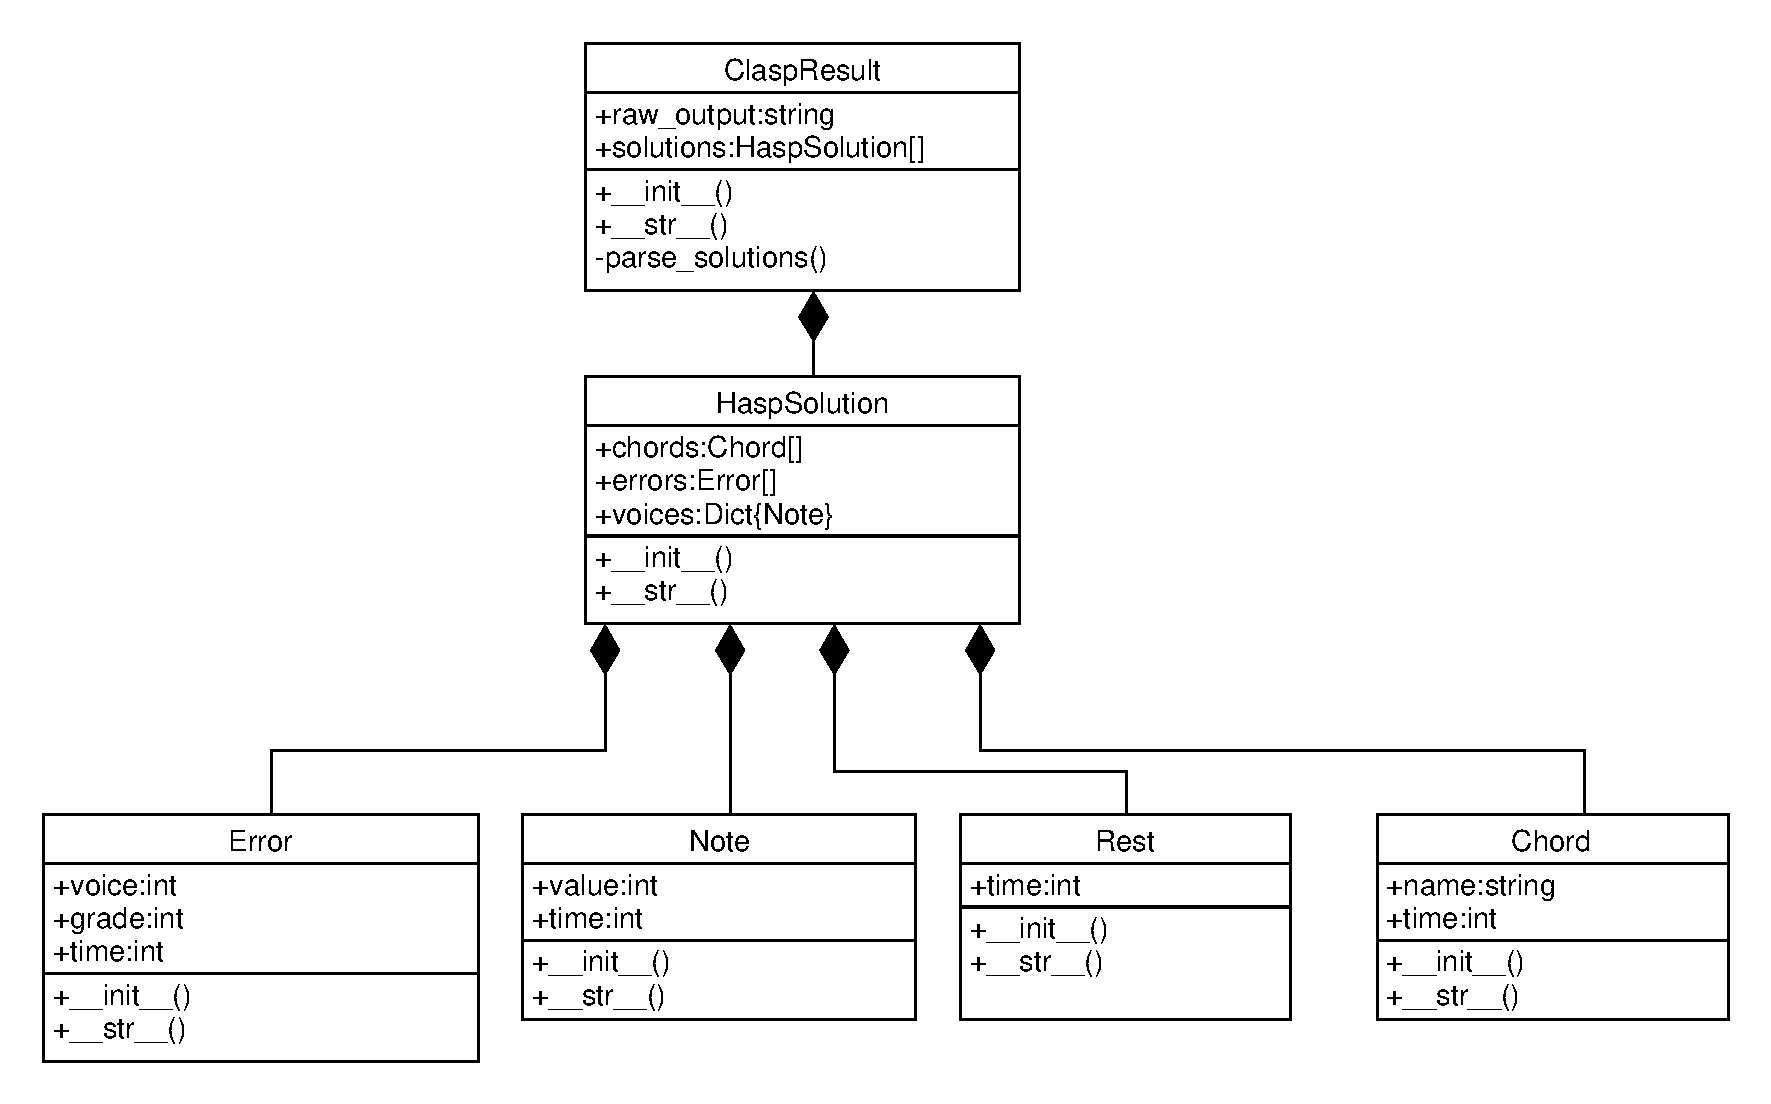
\includegraphics[width=0.8\linewidth]{imagenes/fifth_iter.pdf}
	\caption{Diagrama de clases de almacenamiento de la Iteración 5}
	\label{fig:class_diagram_fifth}
\end{figure}
\begin{figure}[th]
	\centering
	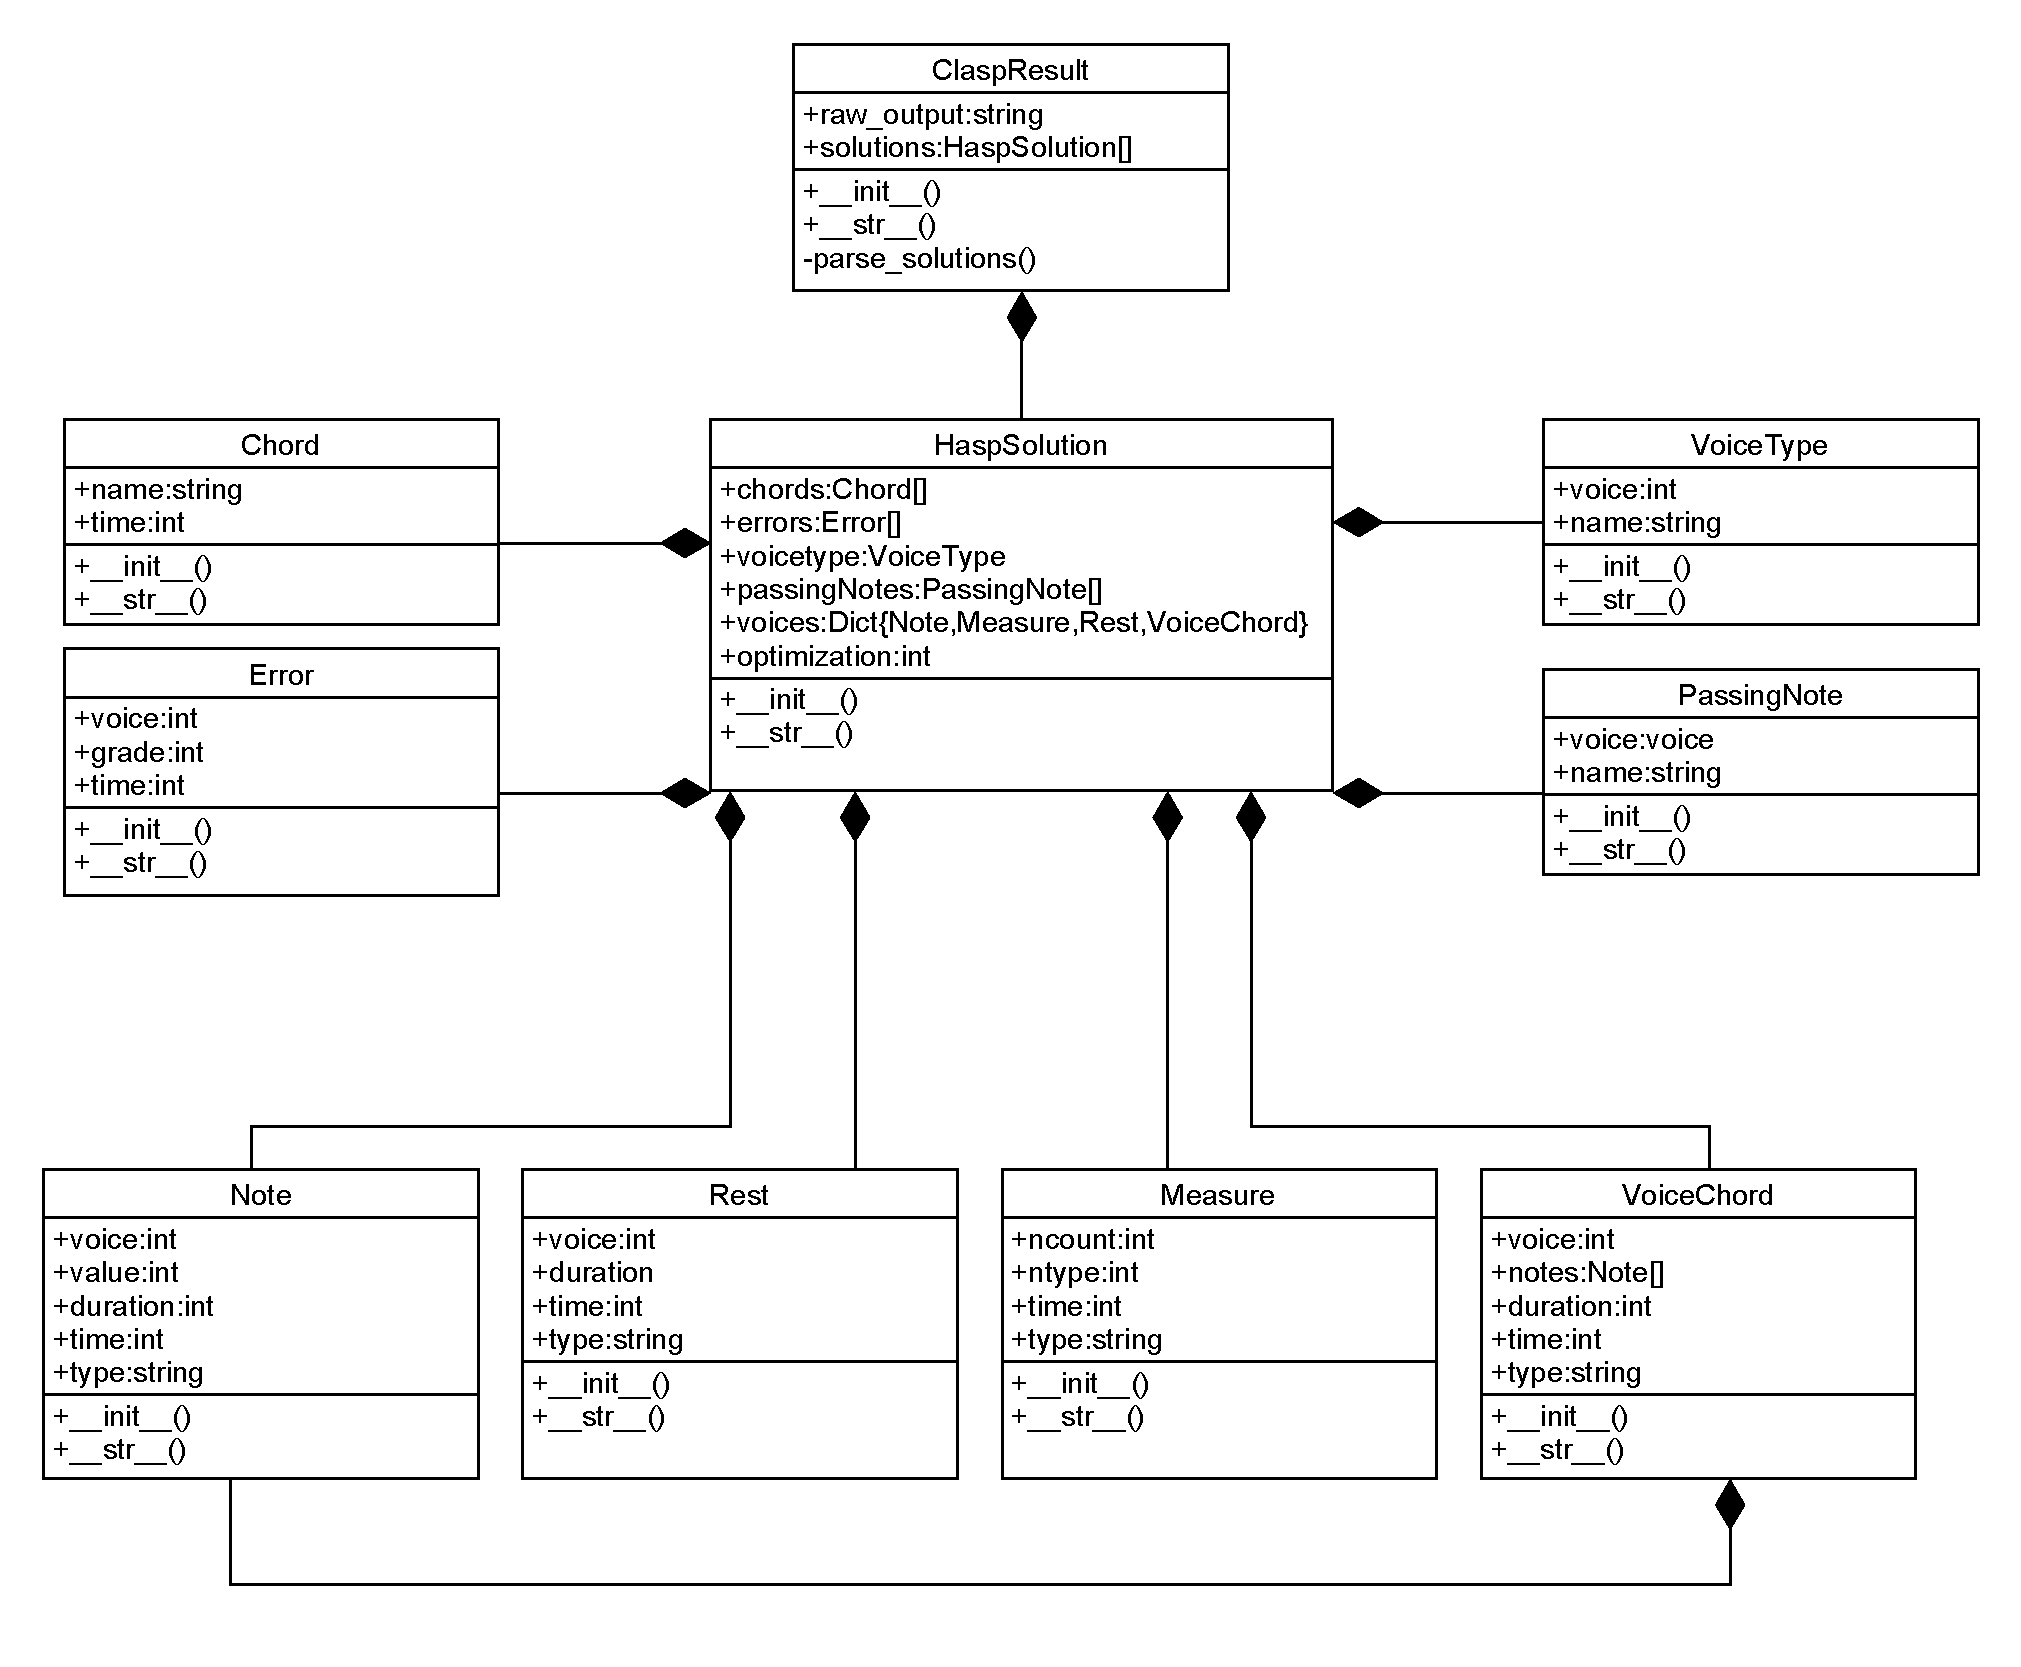
\includegraphics[width=0.8\linewidth]{imagenes/sixth_seventh_eighth_iters.pdf}
	\caption{Diagrama de clases de almacenamiento de las Iteraciones 6, 7 y 8}
	\label{fig:class_diagram_sixth_seventh_eighth}
\end{figure}
\begin{figure}[th]
	\centering
	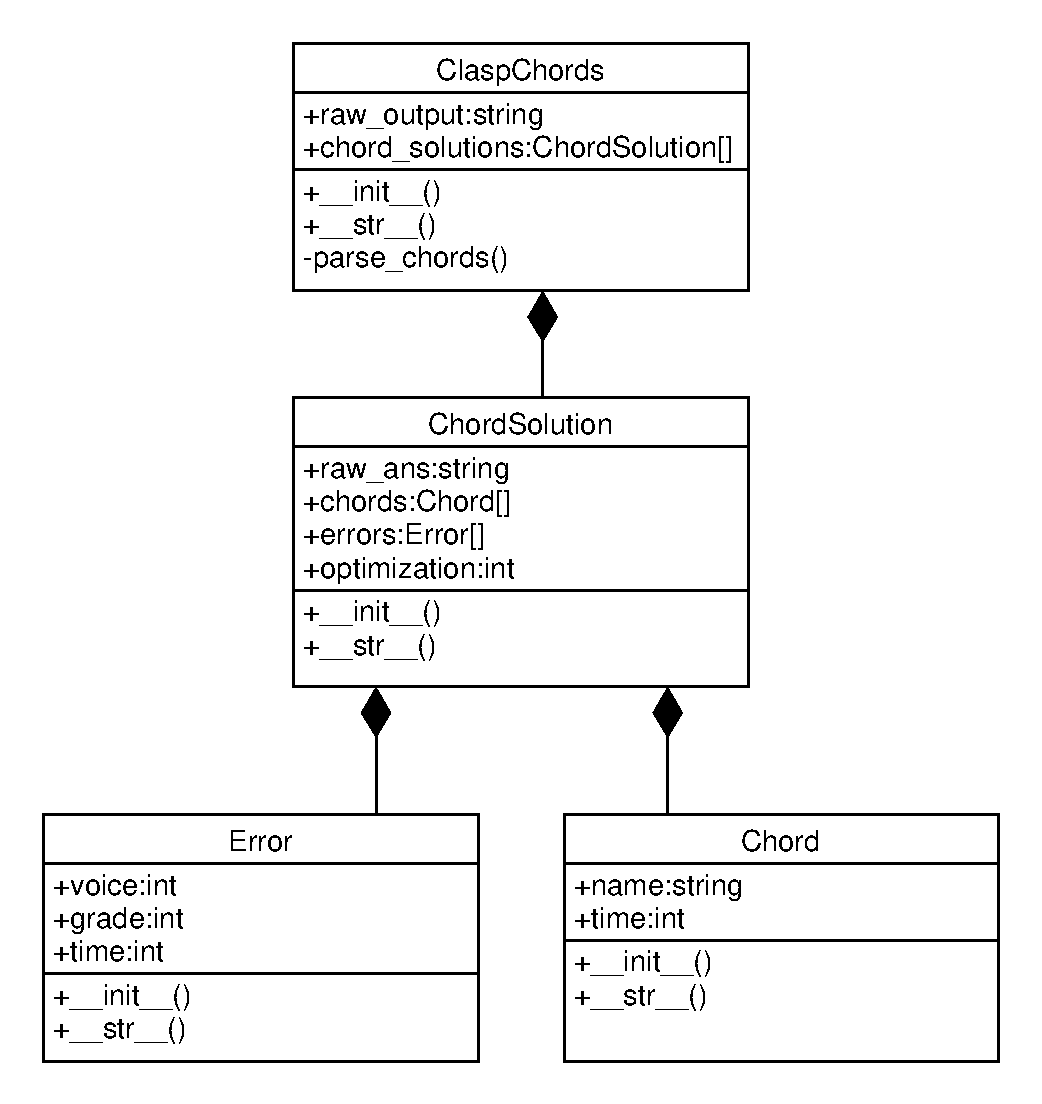
\includegraphics[width=0.8\linewidth]{imagenes/chord_diagram.pdf}
	\caption{Diagrama de clases de almacenamiento del módulo de armonización de la iteración 8}
	\label{fig:class_diagram_chords}
\end{figure}

\chapter{Análisis de MusicXML}
\label{chap:musicxml_analysis}
Se detalla una relación de los elementos MusicXML identificados por el procesador y se especifica la finalidad de los mismos. Se indica también, el tipo de cada elemento procesado (Etiqueta, Etiqueta Autocerrada o Atributo) y, con fines organizativos, la etiqueta con la que están relacionados de forma directa.

 \begin{center}
 	\newcommand*{\TitleParbox}[1]{\parbox[c]{1.75cm}{\raggedright #1}}%
 	\begin{longtable}{ | l | c | c | l | }
 		\hline
 		Nombre & Pertenece a & Tipo & Uso \\ \hline \hline
 		note & measure & Etiqueta & \parbox[l]{6.5cm}{\raggedright Delimita el bloque correspondiente a una nota o silencio} \\ \hline
 		step & note & Etiqueta & \parbox[l]{6.5cm}{\raggedright Especifica el nombre de la nota en notación internacional} \\ \hline
 		octave & note & Etiqueta & \parbox[l]{6.5cm}{\raggedright Indica el número de la octava de la nota} \\ \hline
 		rest & note & Autocerrada & \parbox[l]{6.5cm}{\raggedright Indica si la figura es un silencio, en caso de aparecer, step y octave no se especifican} \\ \hline
 		chord & note & Autocerrada & \parbox[l]{6.5cm}{\raggedright Indica si la nota forma parte de un acorde} \\ \hline
 		type & note & Etiqueta & \parbox[l]{6.5cm}{\raggedright Especifica el tipo de figura mediante un string (whole, half, quarter...)} \\ \hline
 		staff & note & Etiqueta & \parbox[l]{6.5cm}{\raggedright Identifica el número de pentagrama al que pertenece la nota, usado en instrumentos con múltiples pentagramas como el piano} \\ \hline
 		grace & note & Autocerrada & \parbox[l]{6.5cm}{\raggedright Indica si la nota es una apoyatura} \\ \hline
 		alter & note & Etiqueta & \parbox[l]{6.5cm}{\raggedright Especifica el valor de alteración usando números positivos para sostenidos y negativos para bemoles} \\ \hline
 		duration & note & Etiqueta & \parbox[l]{6.5cm}{\raggedright Indica la duración de la figura} \\ \hline
 		dot & note & Autocerrada & \parbox[l]{6.5cm}{\raggedright Indica si la nota está acompañada de un puntillo} \\ \hline
 		part & score-partwise & Etiqueta & \parbox[l]{6.5cm}{\raggedright Delimita los bloques de cada voz o parte de la partitura} \\ \hline
 		score-part & part-list & Etiqueta & \parbox[l]{6.5cm}{\raggedright Delimita los bloques de meta-información de cada una de las partes} \\ \hline
 		instrument & score-part & Etiqueta & \parbox[l]{6.5cm}{\raggedright Especifica el nombre del instrumento la parte correspondiente} \\ \hline
 		print-object & note & Atributo & \parbox[l]{6.5cm}{\raggedright Indica si la nota es visible o no} \\ \hline
 		credit-words & credit & Etiqueta & \parbox[l]{6.5cm}{\raggedright Almacena metadatos sobre autor o título de la partitura} \\ \hline
 		time & attributes & Etiqueta & \parbox[l]{6.5cm}{\raggedright Delimita bloques sobre la información de compases} \\ \hline
 		beats & time & Etiqueta & \parbox[l]{6.5cm}{\raggedright Indica la cantidad de figuras del compás (numerador)} \\ \hline
 		beat-type & time & Etiqueta & \parbox[l]{6.5cm}{\raggedright Indica la figura base del compás (denominador)} \\ \hline
 		harmony & measure & Etiqueta & \parbox[l]{6.5cm}{\raggedright Delimita un bloque que especifica la notación de armonía del compás} \\ \hline
 		root-step & harmony & Etiqueta & \parbox[l]{6.5cm}{\raggedright Indica la nota raíz del acorde que se anota sobre el compás} \\ \hline
 		kind & harmony & Etiqueta & \parbox[l]{6.5cm}{\raggedright Indica el tipo de acorde anotado sobre el compás (mayor, menor, dominante séptima...)} \\ \hline
 		fifths & key & Etiqueta & \parbox[l]{6.5cm}{\raggedright Indica la cantidad de sostenidos o bemoles presentes en la armadura de la partitura. Usa números positivos para los sostenidos y negativos para los bemoles} \\ \hline
 		mode & key & Etiqueta & \parbox[l]{6.5cm}{\raggedright Indica el modo (mayor o menor) de la tonalidad especificada por la armadura de la partitura} \\ \hline
 	\end{longtable}
 \end{center} 
 
 \chapter{Partituras}
 \label{chap:scores}
 Además de las utilizadas en la evaluación del sistema, se utilizaron algunas otras partituras durante el desarrollo del proyecto, algunas descartadas por incompatibilidad y otras por no servir de ejemplo para la evaluación.
 
 \begin{figure}
 	\centering
 	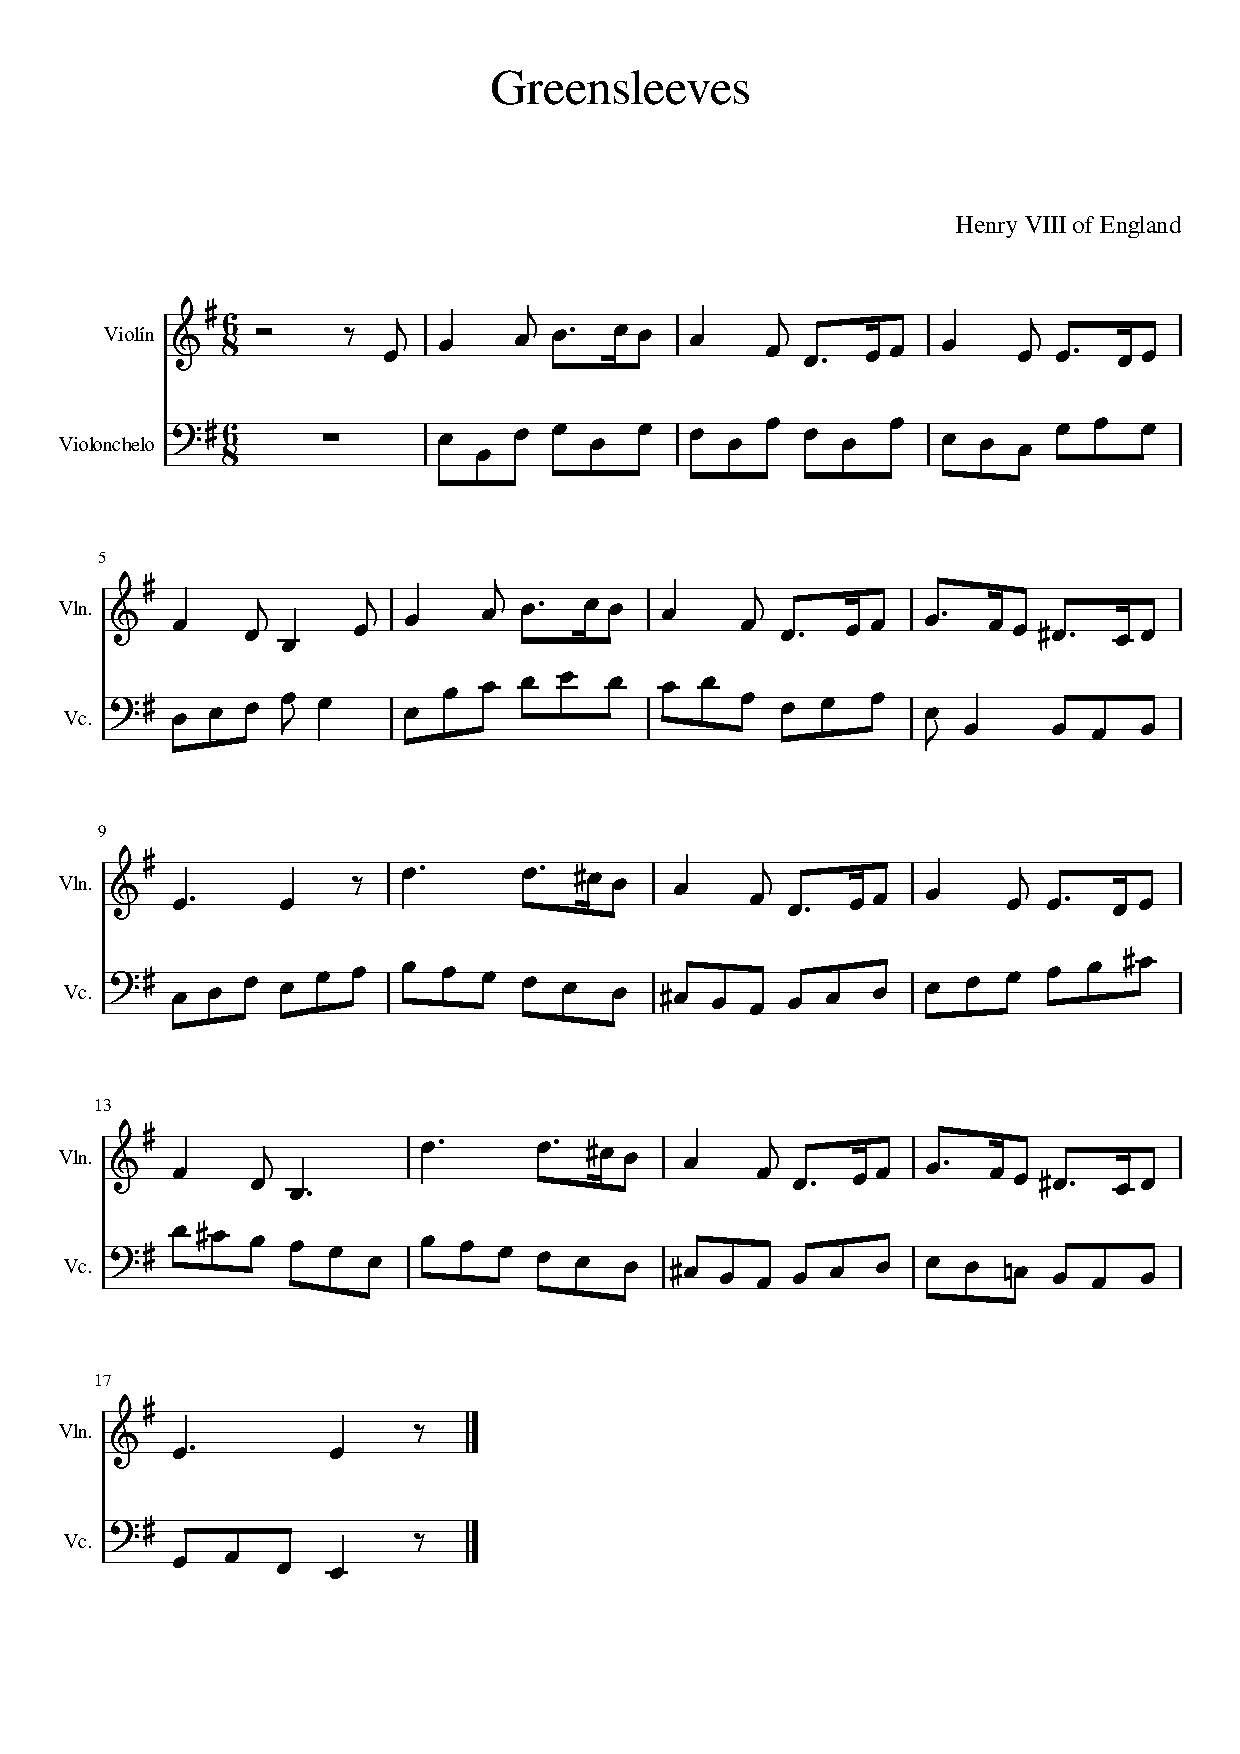
\includegraphics[width=0.8\linewidth]{imagenes/scores/Greensleeves.pdf}
 	\caption{Partitura de Greensleeves, por Enrique VIII}
 	\label{fig:greensleeves_score}
 \end{figure}
 
  \begin{figure}
  	\centering
  	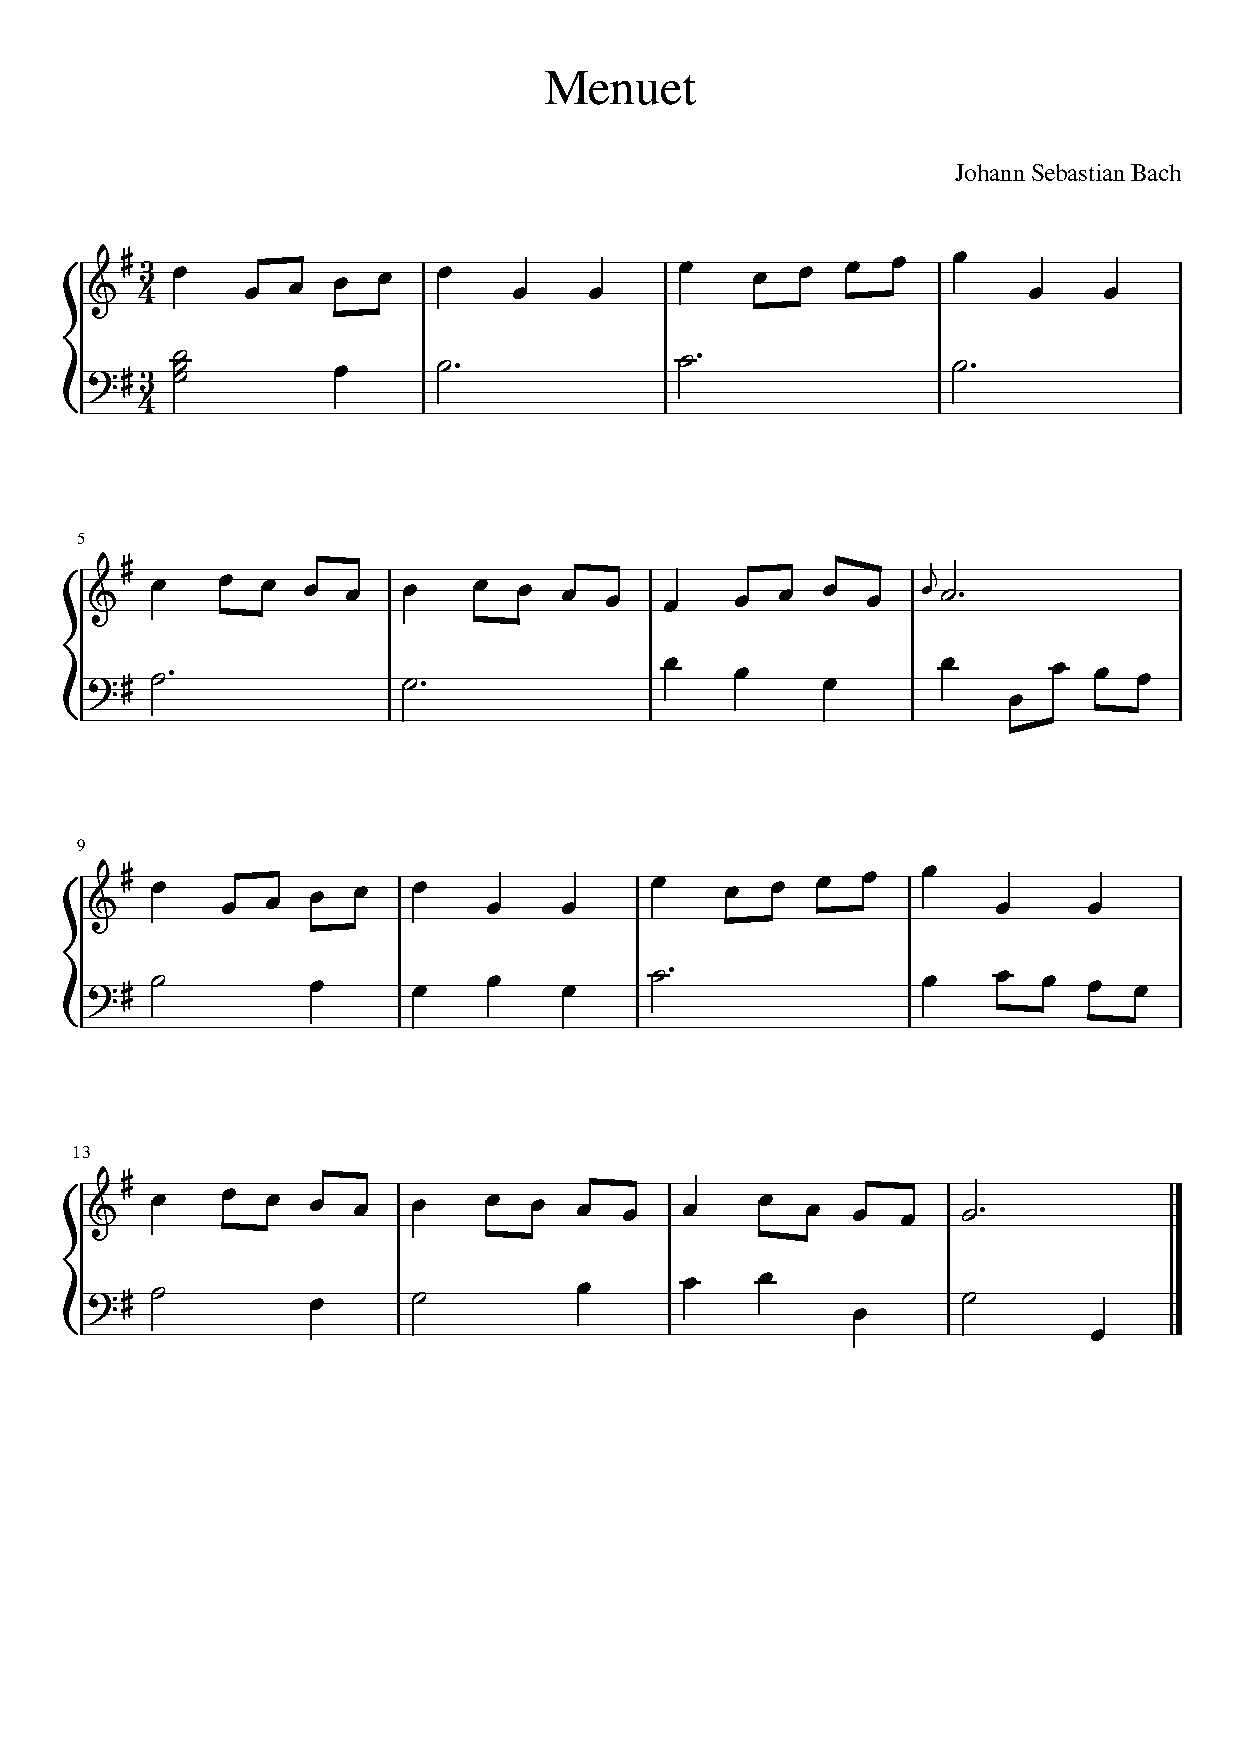
\includegraphics[width=0.8\linewidth]{imagenes/scores/menuet_bach.pdf}
  	\caption{Partitura de Menuet, por Johann S. Bach}
  	\label{fig:menuet_score}
  \end{figure}
  
    \begin{figure}
    	\centering
    	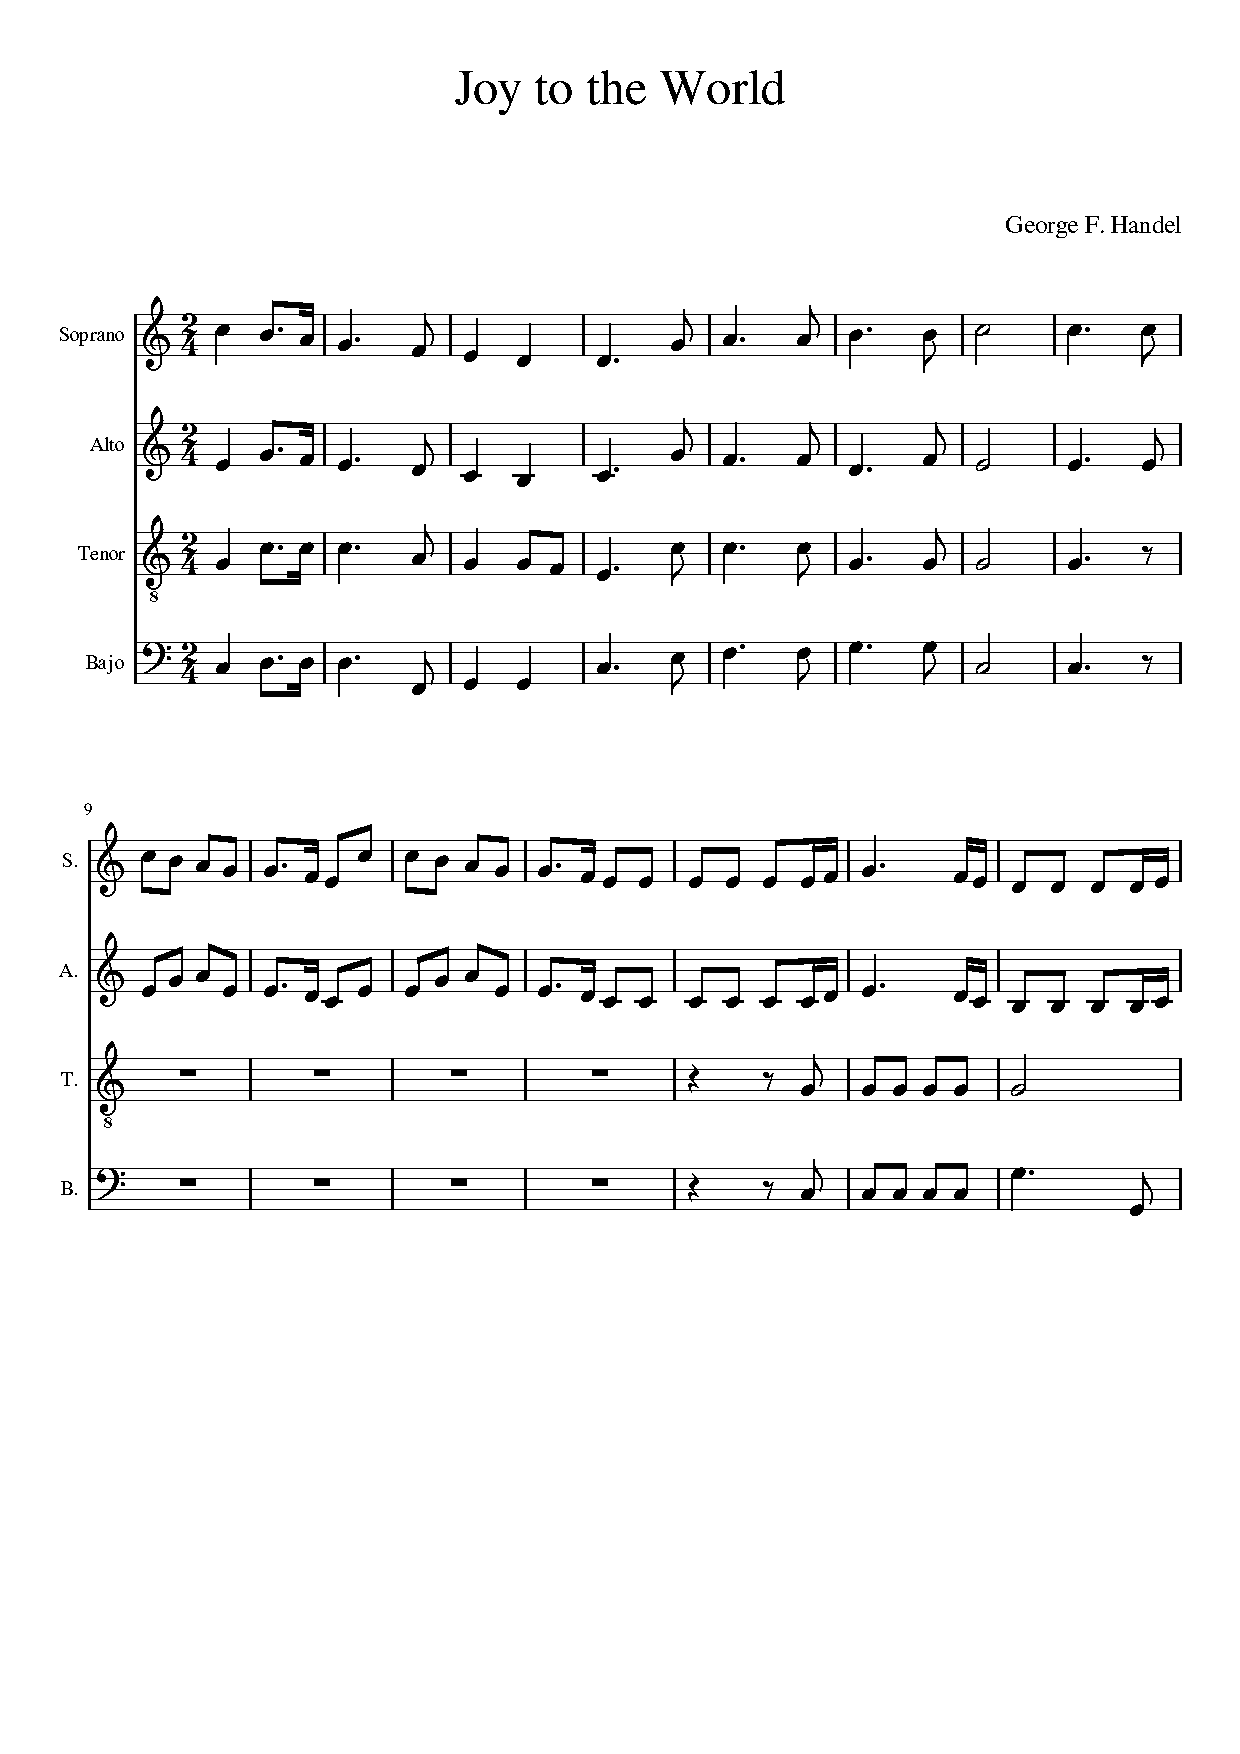
\includegraphics[width=0.8\linewidth]{imagenes/scores/Joy_to_the_World.pdf}
    	\caption{Partitura de Joy to the World, por George F. Handel}
    	\label{fig:joy_score}
    \end{figure}
 
     \begin{figure}
     	\centering
     	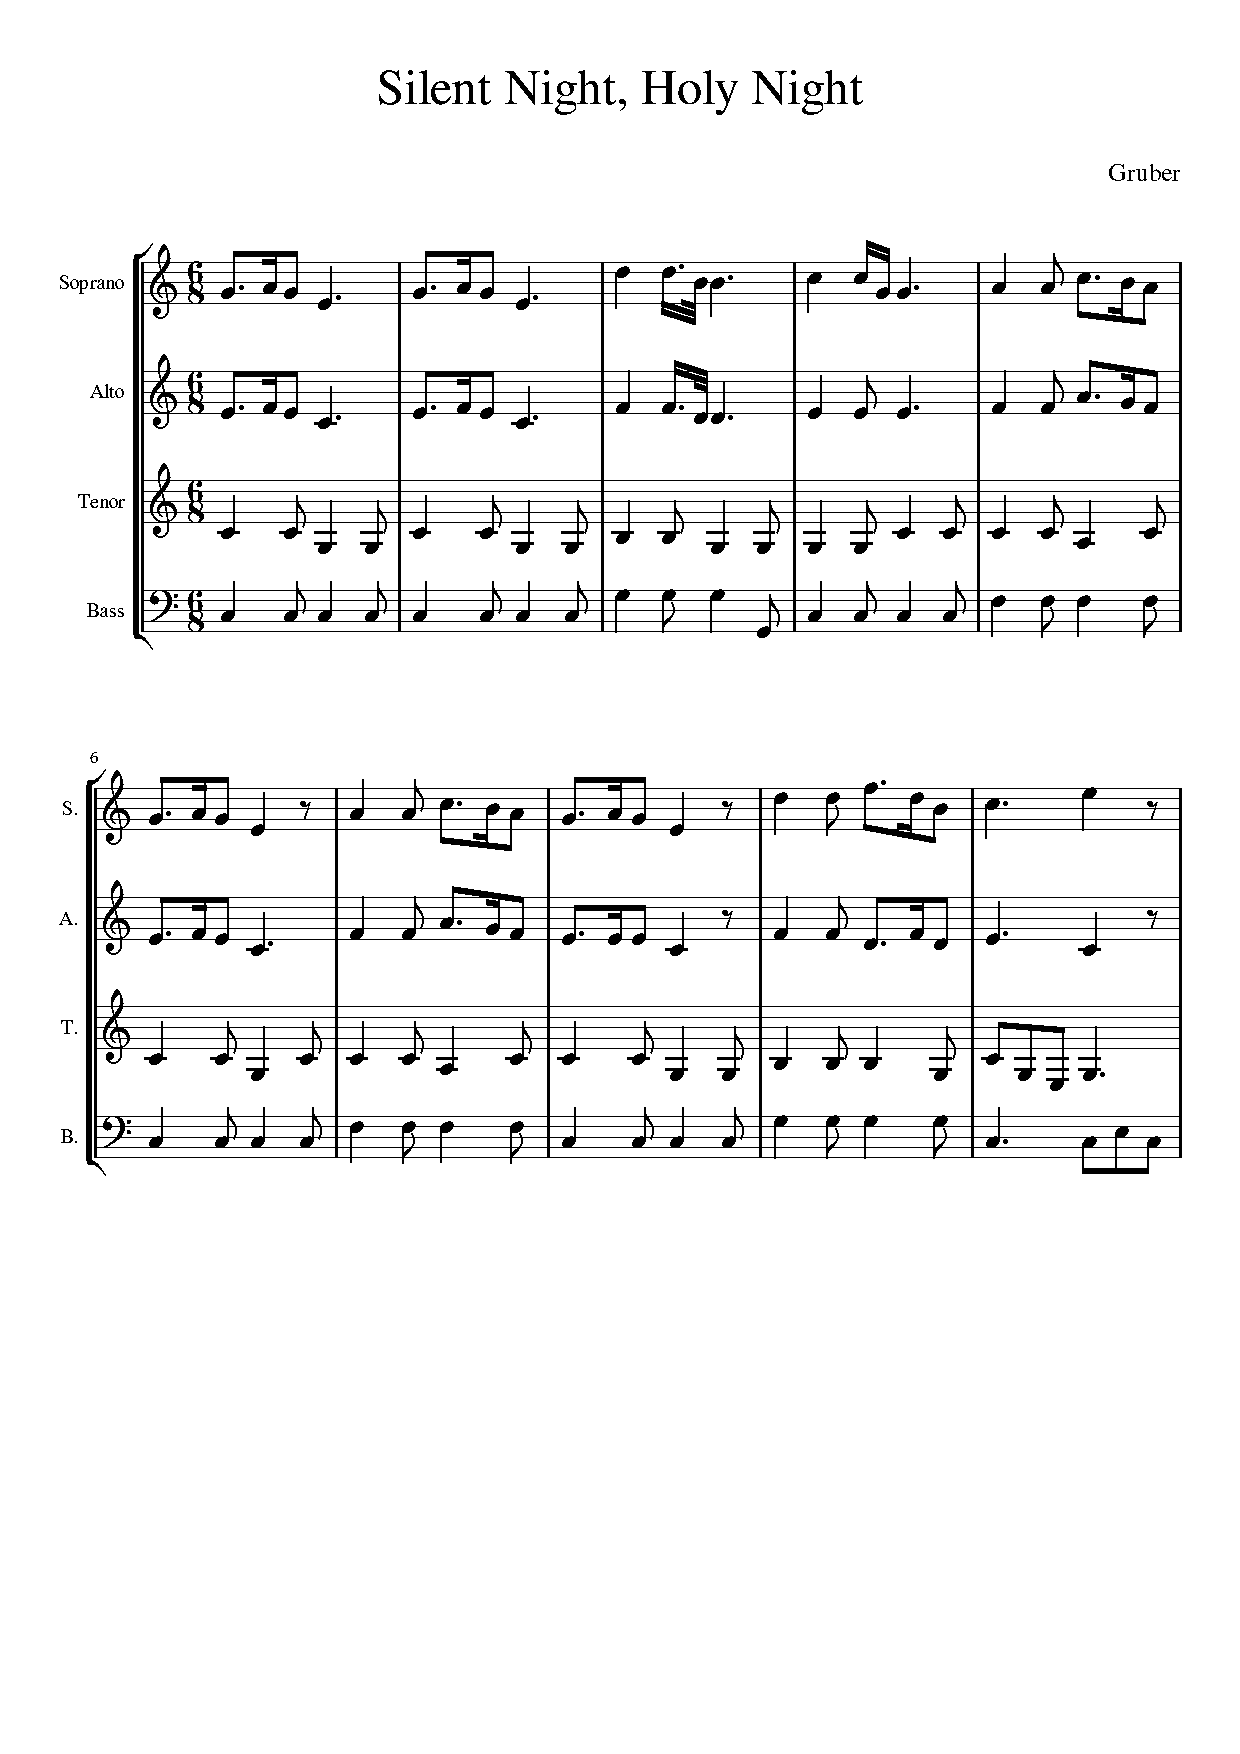
\includegraphics[width=0.8\linewidth]{imagenes/scores/silent_night.pdf}
     	\caption{Partitura de Silent Night (Noche de Paz), por Franz X. Gruber}
     	\label{fig:silent_score}
     \end{figure}
     
          \begin{figure}
          	\centering
          	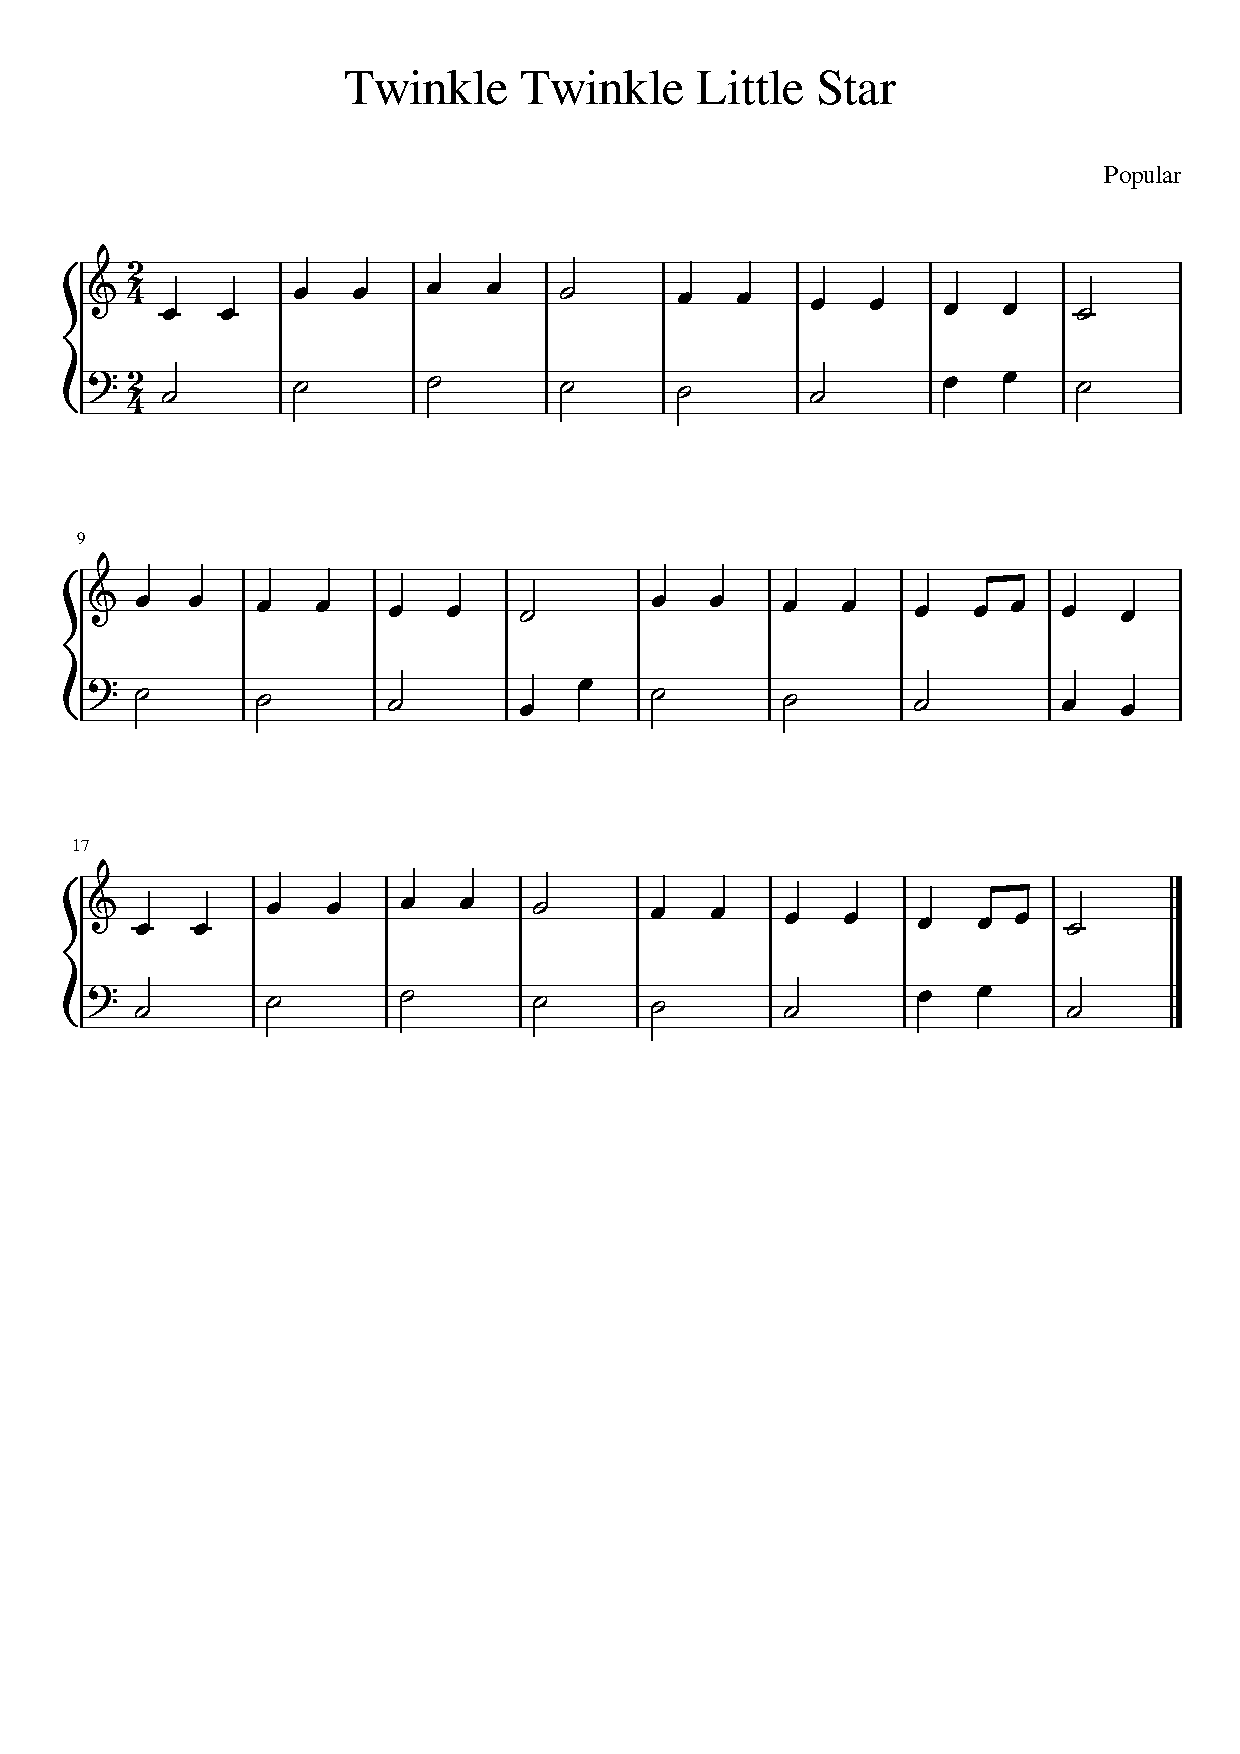
\includegraphics[width=0.8\linewidth]{imagenes/scores/Twinkle_Twinkle_Little_Star.pdf}
          	\caption{Partitura de la pieza popular infantil Twinkle Twinkle Little Star (Brilla Brilla Estrellita)}
          \end{figure}
     
     \begin{figure}
     	\centering
     	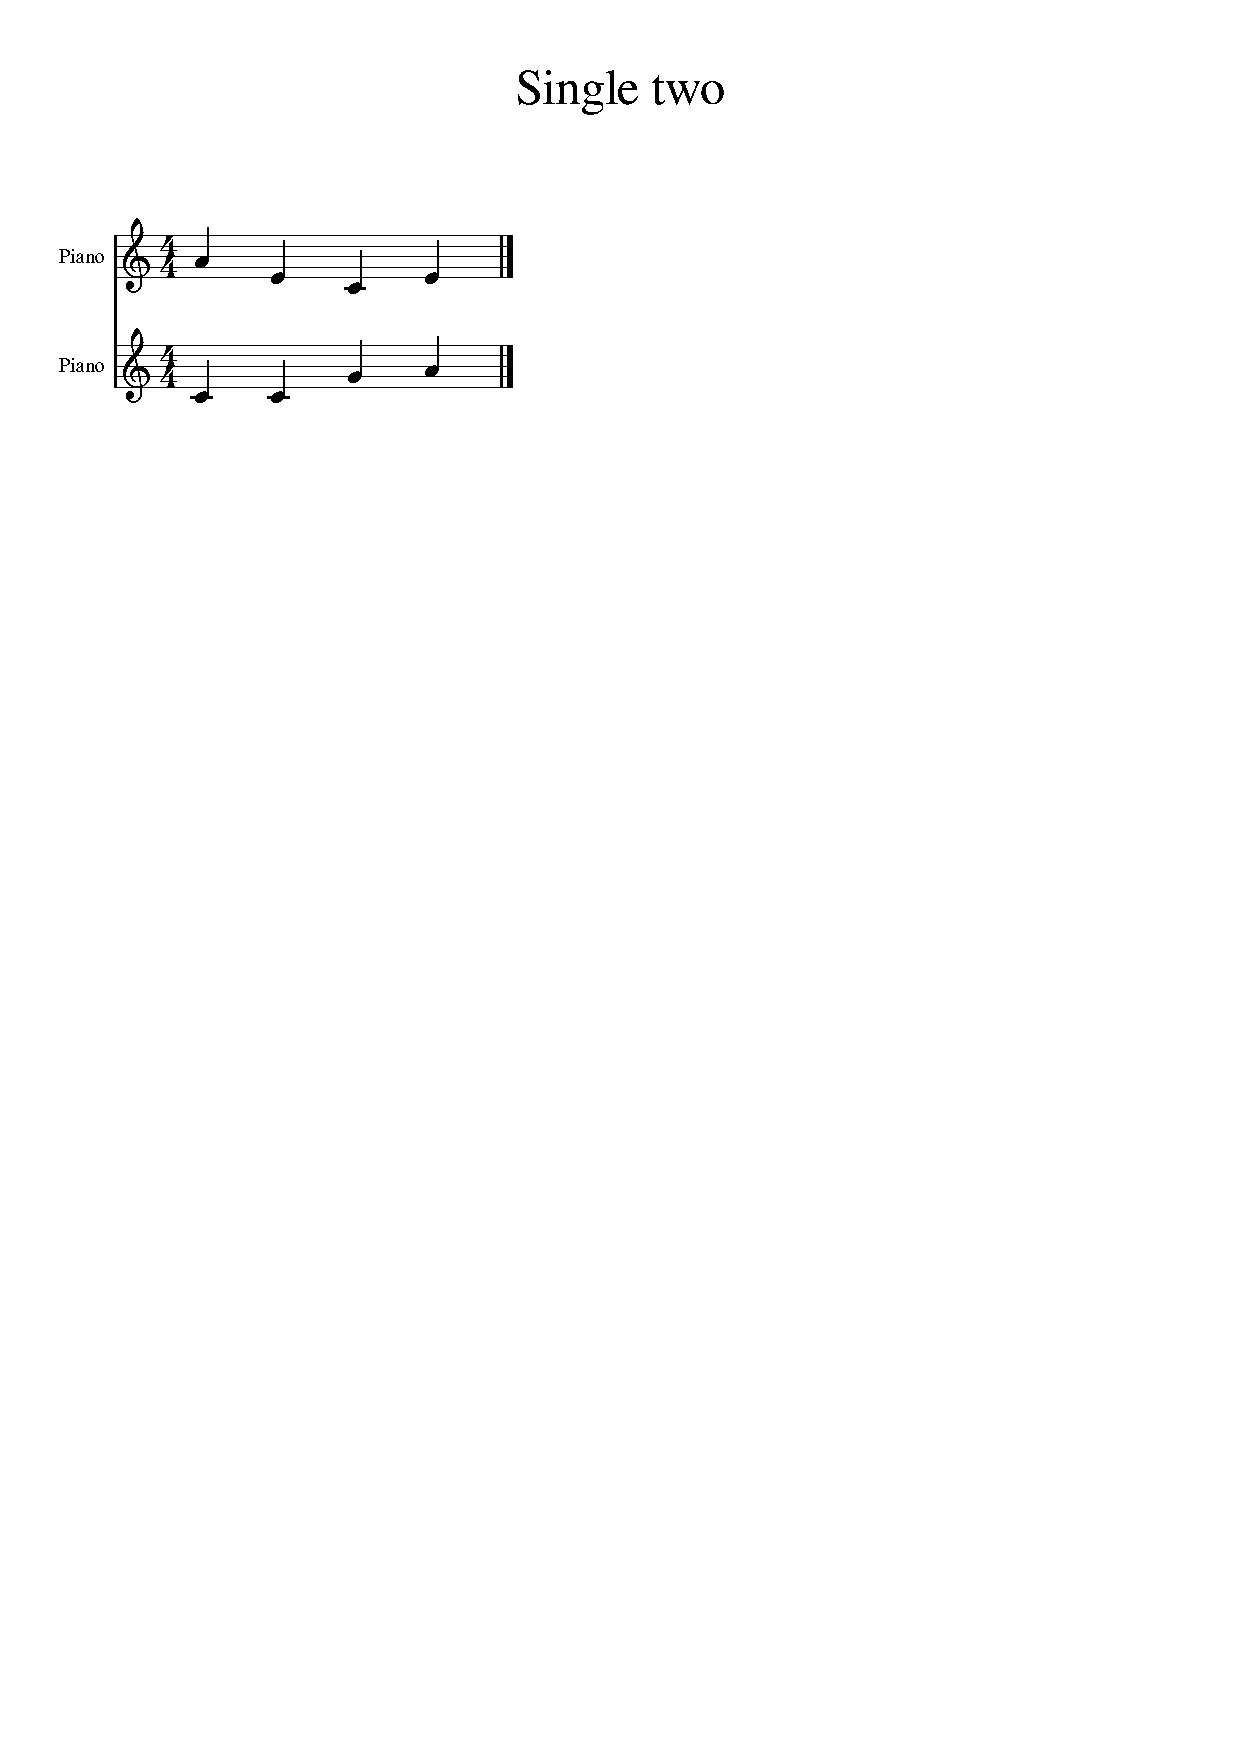
\includegraphics[width=0.8\linewidth]{imagenes/scores/simple_chords.pdf}
     	\caption{Partitura de ejemplo con una serie de acordes sencillos}
     	\label{fig:simplechords_score}
     \end{figure}

 \begin{figure}
 	\centering
 	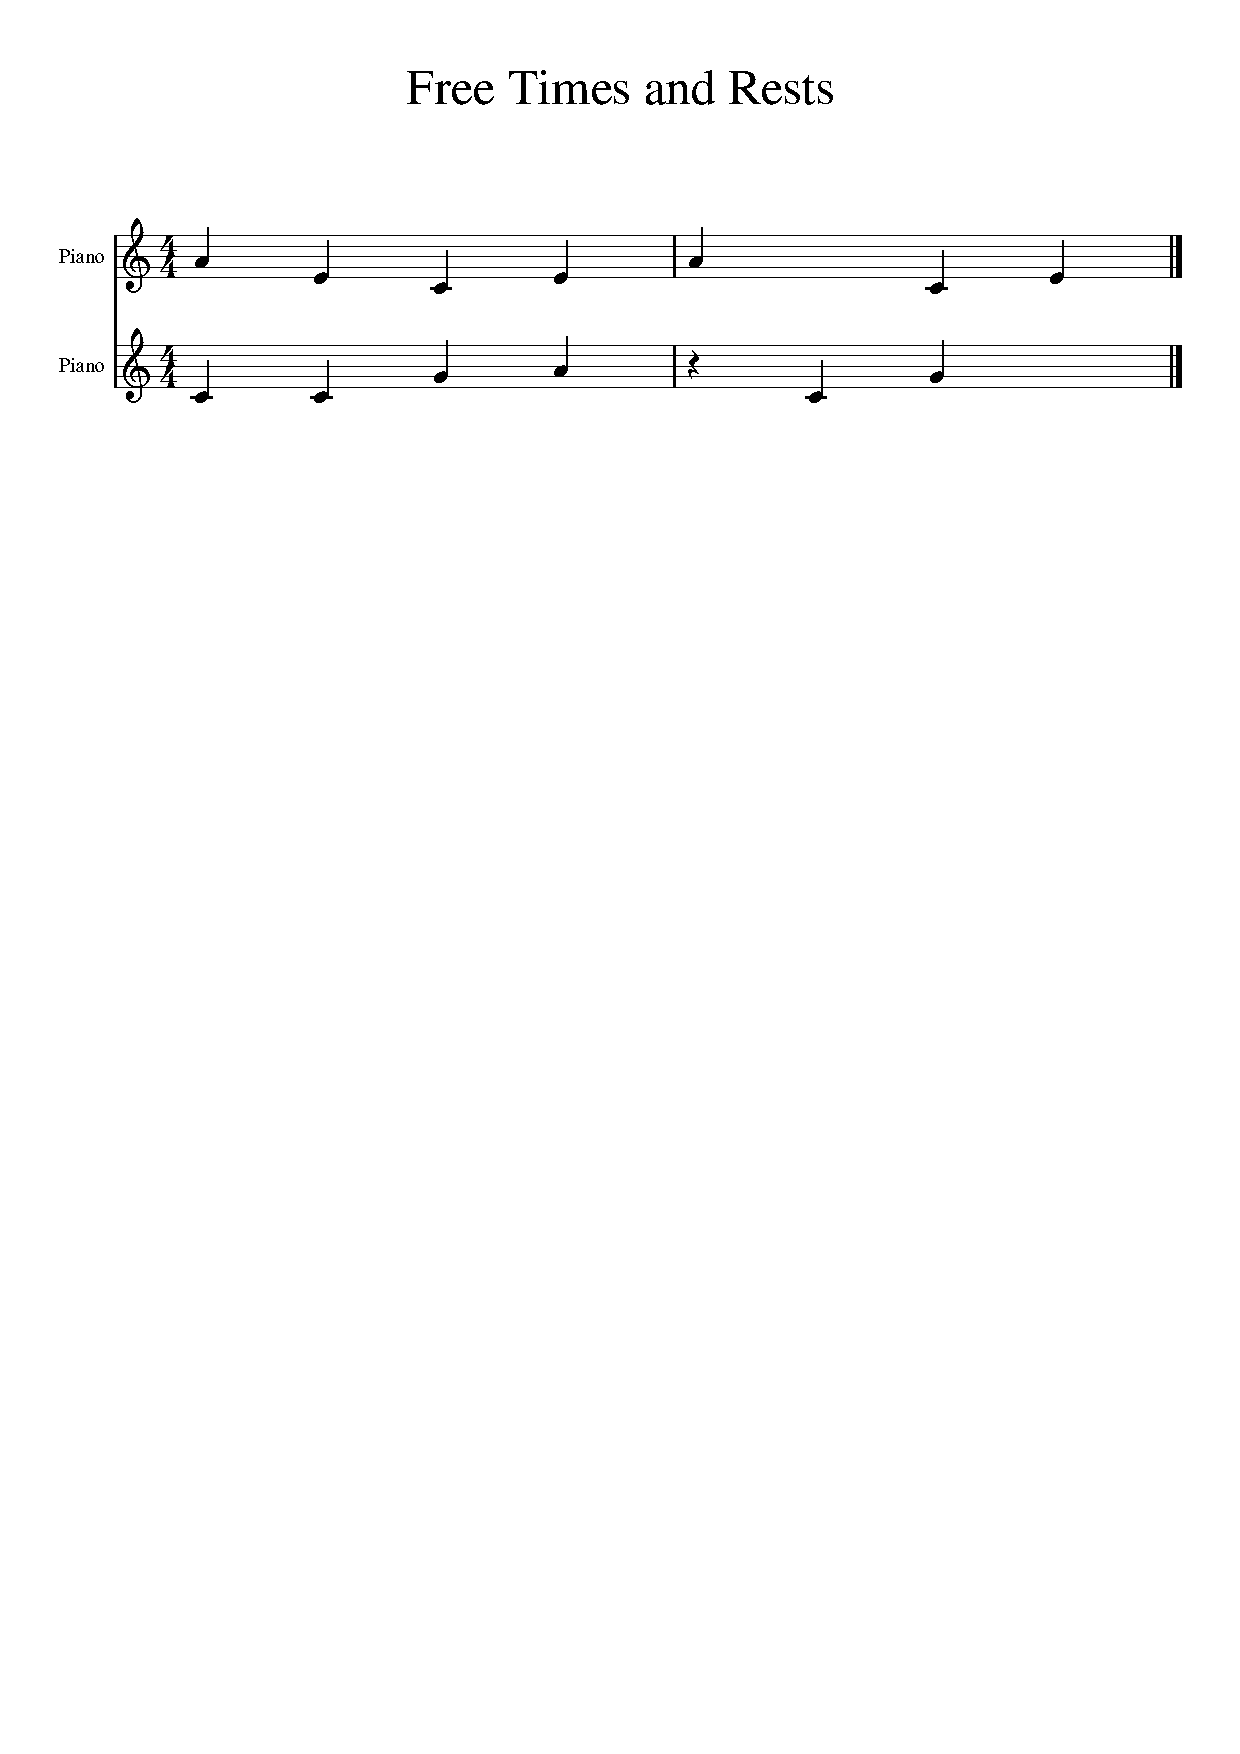
\includegraphics[width=0.8\linewidth]{imagenes/scores/freetimerests.pdf}
 	\caption{Partitura de ejemplo con algunos silencios reales y otros invisibles}
 	\label{fig:rests_score}
 \end{figure}
 
  \begin{figure}
  	\centering
  	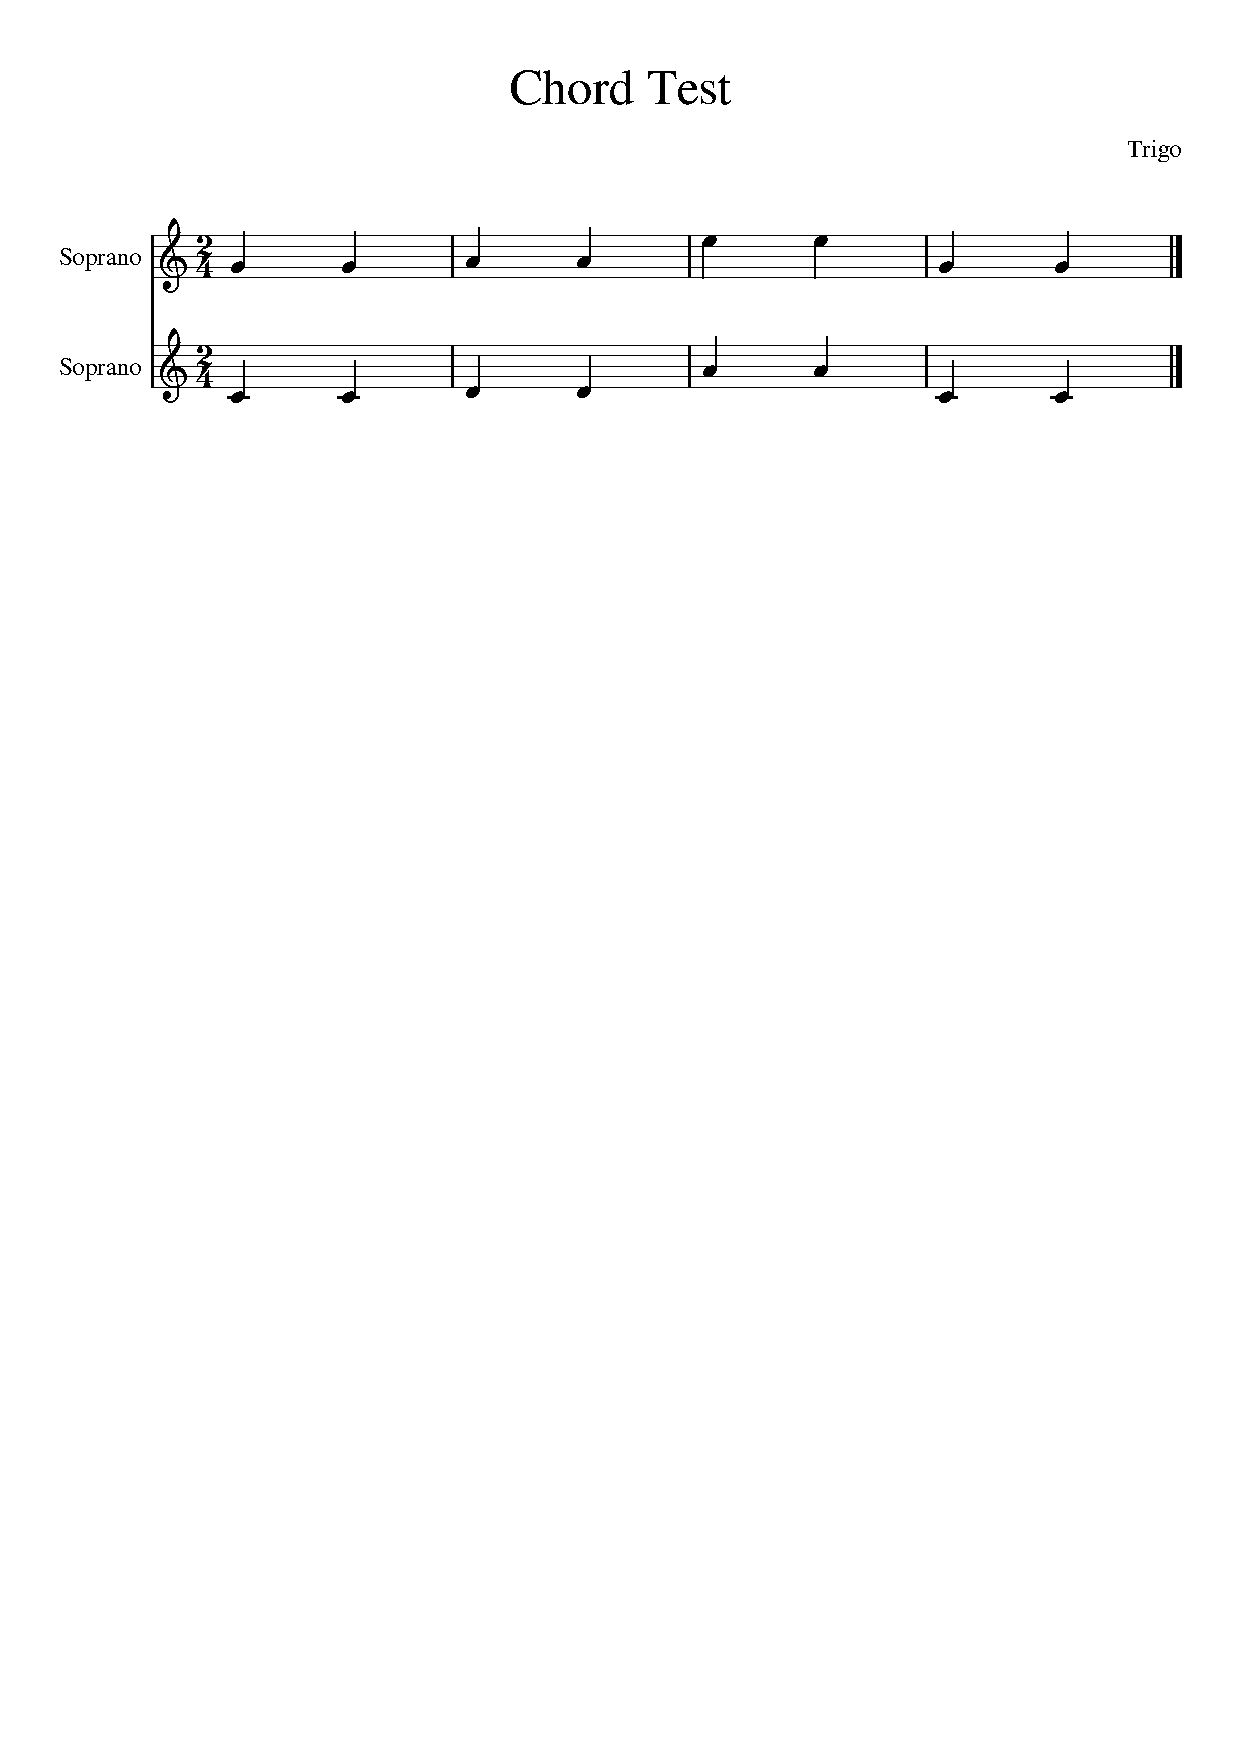
\includegraphics[width=0.8\linewidth]{imagenes/scores/Chord_Test.pdf}
  	\caption{Partitura de ejemplo con acordes definidos por la quinta para ser completada.}
  	\label{fig:chord_test}
  \end{figure}
 
\chapter{Instalación}
\label{chap:installation}
Se recomienda la instalación de la herramienta en un sistema operativo Linux. Esto se debe a que las librerías Flex y Bison se  compilan fácilmente en dicha plataforma. No obstante se proporciona el código fuente completo, por lo tanto es posible compilarlo para otros sistemas operativos.

El requisito es tener instalado Python 2.7, las ultimas versiones de Flex y Bison, además de un compilador de C (gcc sirve perfectamente). A mayores es necesario descargar tanto gringo 3.0.5 como clingo 3.0.5 de la página en Sourceforge del grupo Potassco\cite{potasscoweb} y el módulo Music21 en su versión 2.1.2 o superior de la página de la librería. Todas estas herramientas, compiladores y librerías deben ser accesibles mediante en el \texttt{PATH} del sistema operativo.

La instalación de tanto gringo como clingo no tiene mayor complicación, sólo deben ubicarse en alguna carpeta accesible y añadir dicha ruta al \texttt{PATH}. En la página web de Music21\cite{music21web} se incluyen instrucciones para su instalación automatizada en el sistema. Se aconseja, no obstante instalar primero diferentes herramientas para transformación y visualización o reproducción de los diferentes formatos (Léase PDF, MIDI, Lilypond, etc.) ya que de este modo, la instalación de Music21 las reconocerá y podrán ser usadas sin configuración posterior. Si se desean cambiar las preferencias sobre estas herramientas vinculadas a Music21, ha de editarse el fichero \texttt{.music21rc} presente en la carpeta \texttt{home} del usuario activo del sistema.
	
Se recomienda la instalación de un editor de partituras para poder manipular correctamente los ficheros de entrada y salida de la herramienta, esto es opcional, pero resulta conveniente. En el desarrollo se ha utilizado MuseScore 2 al ser \textit{OpenSource} y gratuito, pero cualquier editor que pueda importar y exportar ficheros en formato MusicXML servirá.

Con la herramienta, además del código fuente, se ofrece el procesador MusicXML a hechos lógicos precompilado, si no funcionase este archivo siempre puede compilarse el mencionado código fuente haciendo uso del archivo Makefile presente en la carpeta \texttt{parser/source}. un simple comando \texttt{make} desde esa ruta es suficiente. El archivo binario compilado del procesador debe estar presente en la carpeta \texttt{parser} para que la herramienta funcione correctamente.

\chapter{Manual de uso}
\label{chap:usage}
Esta herramienta está pensada para ser usada desde la línea de comandos en sistemas operativos Linux. El comando básico para su ejecución es \texttt{python haspie.py <fichero.xml>} y las opciones que permite la herramienta, junto con una pequeña explicación de cada una de ellas, pueden ser invocadas mediante la opción \texttt{-h}, como es habitual. No obstante se detalla una ejecución completa a modo de guía de uso.

\begin{figure}
	\begin{verbatim}
usage: haspie.py [-h] [-n N] [-s S] [-v V [V ...]] [-S] [-f xml|pdf|midi|ly]
                 [-o output/dir/for/file] [-t T] [-k A~G+-?] [-m major|minor]
                 [-M] [-6] [-a] [-O O] [-c config_file_name.lp]
                 XML_SCORE
haspie - Harmonizing music with ASP
positional arguments:
  XML_SCORE             input musicXML score for armonizing
optional arguments:
  -h, --help            show this help message and exit
  -n N, --num_sols N    max number of ASP solutions, by default all of them
  -s S, --span S        horizontal span to consider while harmonizing, this
                        takes in account subdivision, by default 1
  -v V [V ...], --voices V [V ...]
                        extra instruments, these can be input by name or by
                        numerical note range (i.e soprano,guitar,(65,90)...)
                        to leave one of the sides of the range unespecified
                        use 0
  -S, --show            show result in editor instead of writing it to a file
                        in the desired format
  -f xml|pdf|midi|ly, --format xml|pdf|midi|ly
                        output file format for the result
  -o output/dir/for/file, --output output/dir/for/file
                        output file name for the result
  -t T, --timeout T     maximum time (in seconds) allowed to search for
                        optimum when searching for all optimums, by default
                        there is no time limit
  -k A~G+-?, --key A~G+-?
                        key in which the score should be harmonized, if not
                        specified, parser will autodetect it
  -m major|minor, --mode major|minor
                        mode of the scale, if not specified, parser will
                        autodetect it
  -M, --melodious       turns on melodic preferences in ASP for a more melodic
                        result
  -6, --sixthslink      turns on sixth-four chord linking in ASP for a more
                        natural result (very heavy)
  -a, --all_optimums    turns on the search for all optimums when completing
                        and not just the first found, disabled by default
  -O O, --max_optimums O
                        max number of optimum solutions to display in score
                        completion, by default it's 10
  -c config_file_name.lp, --config config_file_name.lp
                        reads preference order and weights for parameters from
                        the desired *.lp file stored in /pref folder
	\end{verbatim}
	\label{fig:usage}
	\caption{Opciones de uso de la herramienta}
\end{figure}

Lo primero que se debe tener en cuenta es que el fichero de entrada debe proporcionarse en formato MusicXML estándar, este tipo de ficheros son uno de los más comunes en intercambio de partituras y no es difícil encontrar la partitura que deseemos armonizar en este formato. De no ser así, casi cualquier herramienta moderna de composición musical por ordenador puede exportar archivos a este formato. Ya que durante el desarrollo del proyecto se ha usado MuseScore 2, las figuras que acompañan esta sección son capturas de esta herramienta. Para opciones similares en otros editores, consúltese el manual de cada uno.

Una vez obtenido el archivo XML que se desea armonizar y/o completar, puede invocarse el comando básico ya mencionado \texttt{haspie.py <fichero.xml>} para obtener una armonización en la que se asignará un acorde a cada tiempo subdividido de la partitura. Es sumamente importante tener en cuenta la subdivisión de las notas de la partitura ya que la herramienta, para funcionar correctamente, subdivide todas las figuras a la nota más breve. Con esta llamada se calculan automáticamente todos los parámetros de armonización de la partitura: Clave y Modo. En la misma consola de comandos se imprime una serie de datos de mayor o menor utilidad para el usuario como el título de la pieza, la clave y modo detectados así como la longitud de la nota más breve de la partitura, usada como subdivisión. 

\begin{figure}[h]
	\centering
	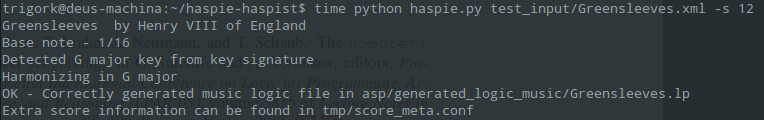
\includegraphics[width=0.8\linewidth]{imagenes/usage/metainfo.png}
	\caption{La información relevante de la partitura se muestra al comenzar la armonización}
	\label{fig:usage_metainfo}
\end{figure}

Tras la armonización se pedirá al usuario que escoja una de las soluciones propuestas por el módulo de armonización. Para esto se muestran todas numeradas y en orden inverso de optimización, siendo las últimas las mejores, de modo que el usuario solo tiene que introducir el número de aquella que desee utilizar. Si sólo se pulsa Enter, se escogerá por defecto la última ya que debería ser mejor (Aunque podría haber varias soluciones empatadas).

\begin{figure}
	\centering
	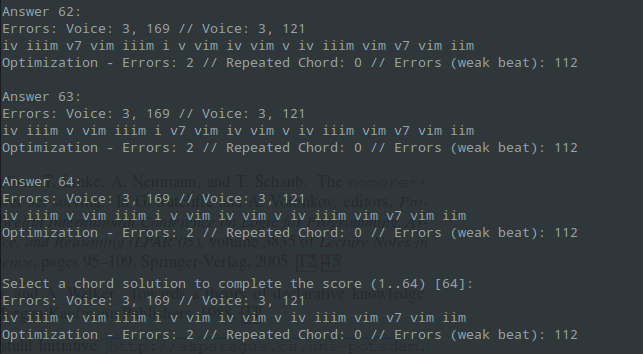
\includegraphics[width=0.8\linewidth]{imagenes/usage/harmony_select.png}
	\caption{Se pide al usuario que fije la armonización a utilizar de entre varias posibles}
	\label{fig:usage_harmony_select}
\end{figure}

A continuación se pasa al módulo de completado de partitura, ya que no se han especificado voces adicionales ni se ha modificado la partitura para contener secciones a completar, no se pedirá escoger una solución de modo similar a la armonización, al existir solo un posible resultado. Finalmente, se genera en la carpeta \texttt{out} el fichero de salida de nombre igual al de entrada, por defecto en formato MusicXML.

De todos modos las armonizaciones más frecuentes no suelen ser a tiempo si no a compás o medio compás. Para cambiar este comportamiento se puede hacer uso de la opción \texttt{-s N} donde \texttt{N} indica la cantidad de tiempos subdivididos que se tomarán en cuenta horizontalmente a la hora de asignar un acorde. Por ejemplo, en la pieza \textit{Joy to the World} se usa un compás \textbf{2/4} (es decir, dos negras por compás), pero la nota más breve de la partitura es una semicorchea, haciendo que la longitud, en semicorcheas, de este compás sea de 8. El cálculo es sencillo de realizar, solo hay que dividir la longitud fraccionaria de la nota más breve entre la longitud fraccionaria del compás y multiplicar este resultado por la cantidad de figuras originales del compás. Para este ejemplo podemos calcular $(16/4)*2=8$.

Normalmente la armadura es un buen indicativo de la clave en la que está escrita la pieza y por tanto de la tonalidad y modo en los que es correcto armonizarla, aun así estos parámetros pueden ser modificados usando \texttt{-k CLAVE} y \texttt{-m major|minor} respectivamente. 
El formato en el que se debe especificar la clave es el nombre internacional de la tonalidad (A-G) junto con un símbolo opcional \texttt{+} o \texttt{-} en caso de querer alterarla con un sostenido o un bemol respectivamente. Modificar estos parámetros alterará drásticamente la armonización de la partitura y los más probable es que si no coinciden con los detectados automáticamente producirá resultados erróneos.

Para modificar el comportamiento del módulo de completado de partituras se puede hacer uso de dos módulos de preferencias adicionales que refinan la salida para obtener un mejor resultado a cambio de requerir más tiempo de búsqueda de las soluciones. Estas preferencias tienen en cuenta las notas presentes en la entrada, pero no las modifican de ningún modo. 
El módulo de preferencias melódicas está orientado a ofrecer unas melodías más suavizadas y pulidas, principalmente minimiza la distancia de los saltos melódicos entre notas de la partitura y realiza un análisis de tendencia de las otras voces para imitar dicha tendencia. Este módulo puede ser utilizado con la opción \texttt{-M}.
El módulo de enlaces de sextas está basado en la detección y enlazado de inversiones de cuarta y sexta de acordes, muy común en polifonía. Este módulo intenta detectar estos patrones y de hallarlos busca que las nuevas notas generadas los continúen. Es signficativamente costoso computacionalmente, puede ser invocado mediante la opción \texttt{-6}.

Para configurar más aún el comportamiento de ambos módulos, la importancia de cada uno de los parámetros que se maximizan o minimizan durante la búsqueda de las mejores soluciones puede ser alterada haciendo uso de ficheros de configuración en formato ASP. En la carpeta \texttt{pref} se encuentra uno comentado con las opciones por defecto. De querer hacer uso de un archivo de configuración solo hay que indicarle la ruta del mismo mediante la opción \texttt{-c /ruta/fichero/config.lp}. 

Cada parámetro de los ficheros de configuración cuenta con dos valores:
\begin{itemize}
	\item \textbf{Peso:} Indicado mediante \texttt{nombre\_weight} mide la importancia de cada uno de estos hechos en el resultado
	\item \textbf{Prioridad:} Indicado mediante \texttt{nombrep} indica el orden en el que se ordenarán las preferencias, a más valor, mayor relevancia en el orden.
\end{itemize}

Para ajustar la cantidad de resultados puede usarse la opción \texttt{-N N}, aunque usarla limitará la búsqueda de resultados a N y no garantiza que se encuentre el mejor valor posible, de no usarse, siempre se explorará todo el espacio de búsqueda.

Para limitar la cantidad máxima de resultados óptimos mostrados por el módulo de completado de partituras puede usarse la opción \texttt{-O O}, ya que al completar puede hallarse una gran cantidad de resultados. A diferencia de \texttt{-N} esta opción solo restringe la cantidad de óptimos mostrados, independientemente de haberse limitado el espacio de búsqueda.

Para controlar el tiempo de ejecución del módulo de completado, ya que este puede dispararse al querer completar grandes secciones puede usarse la opción \texttt{-t tiempo} para expresar cuantos segundos se quiere invertir en la búsqueda. La herramienta siempre usará la cantidad de tiempo especificada, por defecto es 5 segundos.

Existen dos modos de solicitar al módulo de completado de partituras que haga su trabajo:
\begin{itemize}
	\item \textbf{Silencios Completables:} Se realiza mediante un marcado especial en el editor de partituras.
	\item \textbf{Inclusión de voces nuevas:} Se realiza desde la línea de comandos.
\end{itemize}

Los silencios completables son silencios especiales que el procesador interpreta como huecos en vez de como silencios. Para lograr esto se hace uso de una meta-propiedad de las figuras en MusicXML: Su visibilidad. Cualquier figura puede marcarse como invisible desde el panel de propiedades de la figura en el editor, con el fin de que esta no sea impresa en el momento de hacerlo. Esta herramienta entiende los silencios marcados como "no visibles" como huecos a rellenar y la figura utilizada para rellenar dicho espacio será la correspondiente al silencio "no visible" que aparecía originalmente en la partitura.

\begin{figure}[h]
	\centering
	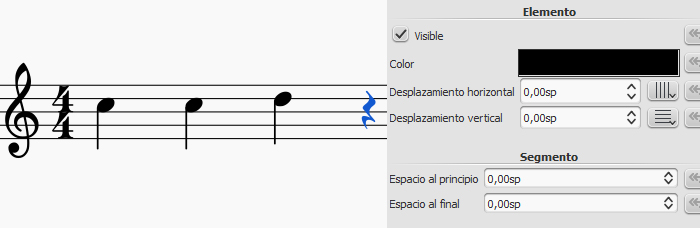
\includegraphics[width=0.8\linewidth]{imagenes/usage/select_silence.jpg}
	\caption{Seleccionando una figura podemos ver sus propiedades, entre otras la casilla de visibilidad}
	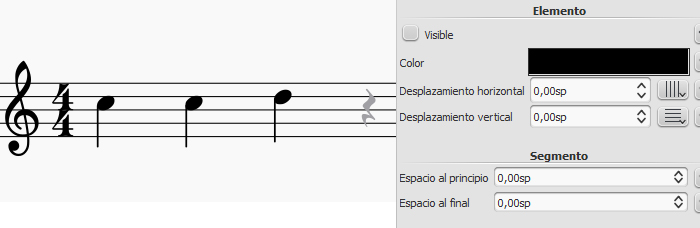
\includegraphics[width=0.8\linewidth]{imagenes/usage/invisible_silence.jpg}
	\caption{Desmarcando la casilla de visibilidad, la figura pasa a un color más claro, indicando que no es visible}
	\label{fig:invisible_silence}
\end{figure}

Las voces nuevas son líneas melódicas completamente vacías originalmente que el módulo de completado se encarga de rellenar respetando la armonía y la tesitura de la voz. Para hacer esto solo hay que usar la opción \texttt{-v voz1 [voz2]...} que toma tantas voces como se quiera añadir como parámetro. Pueden ser especificadas mediante rango de numérico de notas en la forma \texttt{min,max}, usándose 0 si quiere dejarse uno de los extremos abiertos o mediante nombre si la tesitura (o rango de notas) está definida en el fichero \texttt{asp/include/voice\_types.lp}. En éste figuran las tesituras corales más comunes, pero cualquier nuevo instrumento puede ser definido a gusto del usuario.

En caso de requerir completar la partitura de algún modo, tras la armonización, la herramienta solicitará al usuario que escoja la solución que más le guste, mostrando los errores, acordes y notas de cada una de las mejores soluciones halladas.

\begin{figure}
	\centering
	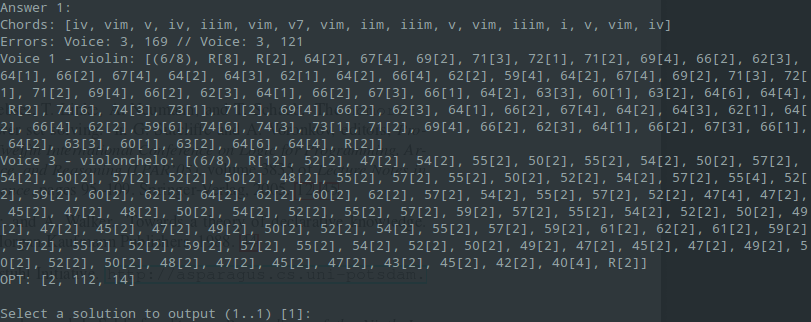
\includegraphics[width=0.8\linewidth]{imagenes/usage/completion_select.png}
	\caption{Se pide al usuario que seleccione la solución que más le guste entre varias posibles}
	\label{fig:usage_completion_select}
\end{figure}

Si se quiere obtener el fichero en algún formato de salida diferente a MusicXML este puede ser especificado mediante \texttt{-f formato}, siempre y cuando se dispongan de herramientas para realizar la conversión instaladas en el sistema. Por ejemplo, para exportar a Lilypond usando \texttt{-f ly} precisaríamos de tener instalado el propio entorno de Lilypond en el sistema. Así mismo se puede cambiar el nombre del fichero de salida con la habitual opción \texttt{-o /ruta/de/salida} (La ruta debe existir).

Por último, si no existiese interés en almacenar el fichero de salida y solo se desease previsualizar el resultado, puede usarse la opción \texttt{-S} para ello. Esto generará un fichero temporal y se ejecutará el software relacionado con la extensión seleccionada para previsualizarlo.

\newpage
\thispagestyle{empty}


 \nocite*
 \bibliography{bibliography}
 \bibliographystyle{IEEEtran}


\end{document}

%%%%%%%%%%%%%%%%%%%%%%%%%%%%%%%%%%%%%%%%%%%%%%%%%%%%%%%%%%%%%%%%%%%%%%%%%%%%%%%%
